\documentclass[a4paper,11pt]{article}
\usepackage[margin=2.6cm]{geometry}
\usepackage{amsmath,amssymb,amsthm,mathtools}
\usepackage{booktabs,graphicx,array,multirow}
\usepackage[hidelinks]{hyperref}
\usepackage{microtype}
\newsavebox{\tabbox}
\newcommand{\fitbox}[1]{\sbox{\tabbox}{#1}\ifdim\wd\tabbox>\textwidth\resizebox{\textwidth}{!}{\usebox{\tabbox}}\else\usebox{\tabbox}\fi}
\usepackage{enumitem}
\usepackage[capitalize]{cleveref}

\usepackage{aliascnt}   % shared theorem counter with correct cleveref names (Proposition/Lemma/Corollary)
\theoremstyle{plain}
\newtheorem{theorem}{Theorem}
\newaliascnt{proposition}{theorem}\newtheorem{proposition}[proposition]{Proposition}\aliascntresetthe{proposition}\crefname{proposition}{Proposition}{Propositions}
\newaliascnt{lemma}{theorem}\newtheorem{lemma}[lemma]{Lemma}\aliascntresetthe{lemma}\crefname{lemma}{Lemma}{Lemmas}
\newaliascnt{corollary}{theorem}\newtheorem{corollary}[corollary]{Corollary}\aliascntresetthe{corollary}\crefname{corollary}{Corollary}{Corollaries}
\theoremstyle{definition}
\newtheorem{definition}{Definition}
\newtheorem{assumption}{Assumption}
\theoremstyle{remark}
\newtheorem{remark}{Remark}
\newtheorem{example}{Example}

\newcommand{\R}{\mathbb{R}}
\newcommand{\Sym}{\mathbb{S}}
\newcommand{\diag}{\operatorname{diag}}
\newcommand{\tr}{\operatorname{tr}}
\newcommand{\lmin}{\lambda_{\min}}
\newcommand{\lmax}{\lambda_{\max}}
\newcommand{\pos}[1]{[#1]_+}
\newcommand{\iprod}[2]{\langle #1,#2\rangle}
\newcommand{\Uth}{U(\theta)}
\DeclareMathOperator*{\argmin}{arg\,min}

\title{Anytime-Certified First-Order Bounds for the Moment--SOS Hierarchy\\ via a Spectral Dual Reformulation}
\author{Tong Chen}
\date{}

\begin{document}
\maketitle

\begin{abstract}
We present \texttt{moment\_sos}, a PyTorch package that turns a polynomial optimization problem into its order-$r$ moment--SOS relaxation and computes \emph{certified upper bounds} with first-order methods. The dual is parametrized by free Gram matrices; repairing each with a diagonal shift sized by an a-priori box bound makes every iterate a valid bound (an anytime certificate), and the infimum of the bound equals the moment relaxation with valid trace cuts, without duality gap. The bound can be re-verified in exact arithmetic. Two solvers share the same eigenvalue oracle: entropic smoothing with L-BFGS and a dual augmented Lagrangian. On order-$2$ MAX-CUT relaxations the method certifies the optimal cut of all $60$ random instances of four Biq Mac-style families ($n\le40$) and of random $3$-regular graphs up to $n=60$ (a $1831\times1831$ moment block, $2.5$\,GiB; about $6$ minutes for each of three $n=60$ instances with a short smoothing schedule; rigorously verified up to $n=40$), where the interior-point solver MOSEK is killed at $n=40$. Interior-point solvers are faster on small blocks, and low-rank or ADMM codes without certificate are faster than ours at every size we tried. As an application we compute second-order relaxations for ReLU-network verification and Lipschitz bounds; they match interior-point values on small networks and tighten the first-order SDP, but our solver does not converge on networks with about $40$ unstable neurons per layer.
\end{abstract}

\section{Introduction}\label{sec:intro}
Polynomial optimization---maximizing a polynomial over a basic semialgebraic set---is NP-hard, yet admits the convergent moment--SOS hierarchy of Lasserre~\cite{lasserre2001} (see also \cite{parrilo2003,laurent2009,nie2023}). Relaxation order $r$ yields an SDP whose moment matrix has size $\binom{n+r}{r}$ and which involves $\binom{n+2r}{2r}$ moment variables. The SDP is dense and highly structured, but general interior-point solvers exploit this structure poorly: their cost is governed by the \emph{number of moments} $m\sim s^2$, not by the matrix size $s$, and they must store an $m\times m$ matrix. For MAX-CUT on $n=40$ nodes at order $r=2$, the moment matrix is only $821\times 821$ but $m=102{,}091$; the interior-point solver MOSEK was killed by the operating system during the optimizer phase on a 36\,GiB machine (\cref{sec:exp}).

\paragraph{Related work and what is new.}
Sparsity exploitation (correlative~\cite{waki2006,lasserre2006}, term~\cite{wang2021tssos,wang2022cstssos}) shrinks the blocks and is complementary to our approach. First-order and low-rank solvers for general SDPs include ADMM-type methods~\cite{odonoghue2016,zheng2020}, sketching-based conditional gradient~\cite{yurtsever2021}, and Burer--Monteiro factorizations~\cite{burer2003}, recently also tailored to moment--SOS relaxations~\cite{hou2025,wang2023manisdp}.
The reduction of SDPs with a trace bound to the minimization of a largest eigenvalue is classical~\cite{helmberg2000,lewis1996}; for the moment--SOS hierarchy it was exploited through the \emph{constant trace property} by Mai, Lasserre, Magron and Wang~\cite{mai2022ctp,mai2023spectral}, who solve the resulting eigenvalue problem with bundle methods. Dathathri et al.~\cite{dathathri2020} introduced the diagonal-domination certificate for neural-network verification.
The established moment--SOS tools construct the SDP and pass it to an interior-point solver: GloptiPoly~3~\cite{henrion2009}, SOSTOOLS~\cite{papachristodoulou2013}, SparsePOP~\cite{waki2008sparsepop}, TSSOS and CS-TSSOS~\cite{magron2021tssos,wang2022cstssos}, and ncpol2sdpa~\cite{wittek2015}. Low-rank and ADMM solvers have been applied to moment relaxations (ManiSDP~\cite{wang2023manisdp}, and a GPU ADMM solver for sparse second-order Lasserre relaxations in trajectory optimization~\cite{kang2024}). To the best of our knowledge (a limited literature and software search, \cref{sec:software}), none of these returns a rigorous a-posteriori bound from the floating-point output of the solver, and we found no PyTorch package for first-order moment--SOS relaxations. We build on the ideas above; the contributions of this paper are the following.
\begin{enumerate}[label=(\alph*),leftmargin=2em]
\item \textbf{A certified spectral dual} (\cref{sec:dual,sec:formal}). A unified free-Gram parametrization of the (sparse) moment--SOS dual for inequalities, equalities, cliques and Boolean variables; every parameter value certifies an upper bound (\cref{thm:certificate}), the infimum equals the moment relaxation with valid trace cuts without duality gap, and equals the Lasserre value for Boolean problems (\cref{thm:exact}); a family of diagonal dominations including the diagonal-cut relaxation (\cref{prop:diag}).
\item \textbf{Solvers and certification} (\cref{sec:algo}). Entropic smoothing with an $O(1/\varepsilon)$ iteration bound (\cref{thm:rate}) and L-BFGS in practice; a smoothing-free dual augmented Lagrangian; integer-valued objectives give optimality proofs (\cref{cor:integer}); a rigorous a-posteriori certificate valid in exact arithmetic (\cref{thm:rigor}); primal recovery with a two-sided certificate for Boolean problems (\cref{prop:primal}).
\item \textbf{Software} (\cref{sec:software}). The PyTorch package \texttt{moment\_sos}: polynomial front end, automatic relaxation, sparsity, tests and documentation.
\item \textbf{A computational study with honest baselines} (\cref{sec:exp,sec:validation}). Agreement with interior-point values; scaling in time and memory up to $n=60$ and order~$3$; comparison with SCS, CGAL and Burer--Monteiro, which are faster but give no certificate; validation of the certificates, primal recovery and cuts.
\item \textbf{Second-order relaxations for ReLU networks} (\cref{sec:nn}): robustness verification and Lipschitz bounds, tighter than the first-order SDP on small networks; partial convergence at $40$ neurons per layer and failure at $60$ variables.
\end{enumerate}

\section{Setting and notation}\label{sec:setting}
We consider
\begin{equation}\label{eq:pop}
f^\star=\max_{x\in K} f(x),\qquad K=\{x\in\R^n:\ g_i(x)\ge0\ (i=1,\dots,p),\ h_j(x)=0\ (j=1,\dots,q)\}.
\end{equation}
\begin{assumption}[box]\label{ass:box}
We work on $K_{\rm box}:=K\cap[-1,1]^n$, i.e.\ $f^\star:=\max_{K_{\rm box}}f$ (no loss of generality after rescaling; if $K\subseteq[-1,1]^n$ then $K_{\rm box}=K$). The box inequalities $1-x_i^2\ge0$ may or may not be among the $g_i$; the relaxations are built from the listed $(g_i,h_j)$ only, and the box enters through the trace and diagonal bounds. In the statements below $K$ and ``feasible'' refer to $K_{\rm box}$.
\end{assumption}
In the \emph{Boolean case} $K\subseteq\{\pm1\}^n$ and all computations are done modulo the ideal $\langle x_i^2-1\rangle$: monomials are squarefree and products are symmetric differences of supports.

\paragraph{Cliques.} Let $I_1,\dots,I_N\subseteq[n]$ be index sets (a single clique $I_1=[n]$ is the dense case) such that the support of every $g_i,h_j$ lies in some clique and every monomial of $f$ is a product of two monomials of one clique. For each clique, $v_k$ denotes the vector of monomials in $x_{I_k}$ of (squarefree) degree $\le r$, $s_k=|v_k|$. For an inequality $g_i$ assigned to clique $k$, $\omega_i=\lceil\deg g_i/2\rceil$ and $z_i$ is the vector of monomials in $x_{I_k}$ of degree $\le r-\omega_i$, with $s_i=|z_i|$. For an equality $h_j$, $\mathcal M_j$ is the set of monomials in the clique of degree $\le 2r-\deg h_j$. We require $\deg f\le 2r$. Let
\begin{equation}\label{eq:B}
B_i:=\sum_{\alpha:\,c_\alpha>0}c_\alpha+\sum_{\alpha:\,c_\alpha<0,\ \alpha\ \text{not even}}|c_\alpha|\ \ \ge \sup_{[-1,1]^n}g_i\quad\text{for } g_i=\sum_\alpha c_\alpha x^\alpha,
\end{equation}
(in the Boolean case every non-constant monomial counts with $|c_\alpha|$). The bound \eqref{eq:B} is a valid and automatable upper bound on $\sup g_i$ over the box, and it is sharper than the usual $\sum_\alpha|c_\alpha|$; e.g.\ $B=1$ for $g=1-x^2$.

\paragraph{Moment relaxation.} For a vector $y$ indexed by monomials, $L_y$ is the linear functional with $L_y(x^\gamma)=y_\gamma$; $M_k(y)=L_y(v_kv_k^\top)$ and $M_i^{\rm loc}(y)=L_y(g_iz_iz_i^\top)$ are the moment and localizing matrices. The (sparse) order-$r$ Lasserre relaxation $\rho_r$ maximizes $L_y(f)$ subject to $y_0=1$, $M_k(y)\succeq0$, $M^{\rm loc}_i(y)\succeq0$, $L_y(h_jx^\mu)=0$ for $\mu\in\mathcal M_j$. We denote by $\rho_r^{\rm tr}$ the same problem with the additional cuts
\begin{equation}\label{eq:cuts}
\tr M_k(y)\le s_k,\qquad \tr M_i^{\rm loc}(y)\le s_iB_i,
\end{equation}
which hold for every moment vector of a probability measure on $K$ because $|x^\alpha|\le1$ on the box and $0\le g_i\le B_i$ on $K$. Hence $f^\star\le\rho_r^{\rm tr}\le\rho_r$. In the Boolean case $M_k(y)_{aa}=y_0=1$ for every $a$, so $\tr M_k=s_k$ \emph{identically} (``constant trace'') and the first cut is redundant.

\begin{table}[t]\centering\small
\setlength{\tabcolsep}{4pt}\renewcommand{\arraystretch}{1.1}
\begin{tabular}{@{}p{3.1cm} p{11.9cm}@{}}\toprule
symbol & meaning\\\midrule
$f,\ g_i,\ h_j,\ K$ & objective, inequality and equality constraints, feasible set of \eqref{eq:pop}; $f^\star=\max_{K_{\rm box}}f$\\
$r,\ I_k,\ v_k,\ s_k$ & relaxation order; clique $k$; monomial vector of degree $\le r$ in $x_{I_k}$; its length\\
$z_i,\ \omega_i,\ B_i$ & monomial vector and half-degree for the localizing block of $g_i$; upper bound of $g_i$ on the box \eqref{eq:B}\\
$y,\ M_k(y),\ M_i^{\rm loc}(y)$ & moment vector, moment and localizing matrices\\
$\rho_r,\ \rho_r^{\rm tr}$ & value of the order-$r$ relaxation, without and with the trace cuts \eqref{eq:cuts}\\
$\theta=(\sigma,Q,p)$ & dual point: scalar, (non-PSD) Gram matrices $Q_{0,k},Q_i$, multiplier polynomials $p_j$\\
$U(\theta),\ U^{\rm d}(\theta)$ & certified upper bound \eqref{eq:U}; diagonal-shift variant (\cref{prop:diag})\\
$\lmin,\ \pos{\cdot},\ \Phi_k$ & smallest eigenvalue; positive part; shift of block $k$ (no positive part for Boolean cliques)\\
$\eta,\ U_\eta$ & entropic smoothing parameter and smoothed bound (\cref{sec:algo})\\
$\rho,\ \rho_0,\ X_b,\ t_b$ & ALM penalty parameter and its start, multiplier and uniform shift of block $b$ (\cref{sec:alm}); not to be confused with the relaxation values $\rho_r$\\
\bottomrule\end{tabular}
\caption{Main notation.}\label{tab:notation}
\end{table}

\section{Gram certificates and the spectral dual}\label{sec:dual}
\begin{definition}[dual point]\label{def:theta}
A \emph{dual point} $\theta$ consists of a scalar $\sigma$, symmetric matrices $Q_{0,k}\in\Sym^{s_k}$, $Q_i\in\Sym^{s_i}$ (not required to be positive semidefinite) and polynomials $p_j\in\operatorname{span}\mathcal M_j$ such that, modulo the ideal in the Boolean case,
\begin{equation}\label{eq:identity}
\sigma-f \;=\; \sum_{k}v_k^\top Q_{0,k}v_k+\sum_{i}\big(z_i^\top Q_iz_i\big)g_i+\sum_jp_jh_j .
\end{equation}
\end{definition}
Writing $\mu_{\min}(Q)=-\lmin(Q)$ and $\Phi(Q)=\pos{-\lmin(Q)}$, define the \emph{spectral bound}
\begin{equation}\label{eq:U}
U(\theta)=\sigma+\sum_ks_k\,\Phi_k(Q_{0,k})+\sum_is_iB_i\,\pos{-\lmin(Q_i)},
\end{equation}
where $\Phi_k(Q)=-\lmin(Q)$ (without the positive part) if clique $k$ is Boolean and $\pos{-\lmin(Q)}$ otherwise.

\begin{theorem}[certificate]\label{thm:certificate}
Under \cref{ass:box}, $f(x)\le U(\theta)$ for all $x\in K$ and all dual points $\theta$. Hence $f^\star\le U(\theta)$.
\end{theorem}
\begin{proof}
Fix $x\in K$ and $\lambda_k=\Phi_k(Q_{0,k})$. Then $Q_{0,k}+\lambda_kI\succeq0$, so $v_k^\top Q_{0,k}v_k\ge-\lambda_k\|v_k\|^2$. On the box $\|v_k(x)\|^2=\sum_a x^{2a}\le s_k$; in the Boolean case $\|v_k(x)\|^2=s_k$ exactly, so the inequality $v_k^\top Q_{0,k}v_k\ge-\lambda_ks_k$ holds even if $\lambda_k<0$. For an inequality, put $\mu_i=\pos{-\lmin(Q_i)}\ge0$; since $g_i(x)\in[0,B_i]$ and $\|z_i\|^2\le s_i$, $(z_i^\top Q_iz_i)g_i\ge-\mu_i\|z_i\|^2g_i\ge-\mu_is_iB_i$. Equality terms vanish on $K$. Evaluating \eqref{eq:identity} at $x$ gives $\sigma-f(x)\ge-\sum_ks_k\lambda_k-\sum_is_iB_i\mu_i$.
\end{proof}

\begin{theorem}[exactness; no duality gap]\label{thm:exact}
Under \cref{ass:box} and if $K\ne\emptyset$,
\[
\inf_\theta U(\theta)=\rho_r^{\rm tr},\qquad f^\star\le\rho_r^{\rm tr}\le\rho_r .
\]
The primal problem $\rho_r^{\rm tr}$ attains its maximum. In the Boolean case $\rho_r^{\rm tr}=\rho_r$. If some optimal solution of $\rho_r$ satisfies the trace cuts \eqref{eq:cuts}, then $\rho_r^{\rm tr}=\rho_r$. If the quadratic module of the $g_i,h_j$ is Archimedean (e.g.\ if $1-x_i^2\ge0$ are among the constraints), then $\rho_r^{\rm tr}\to f^\star$ as $r\to\infty$ (for $r\ge\max_i\omega_i$; for cliques under the running-intersection property~\cite{lasserre2006}); monotonicity of $\rho_r^{\rm tr}$ in $r$ is not claimed, because the cuts of order $r$ do not imply those of order $r-1$.
\end{theorem}
\begin{proof}
See \cref{app:proofs}.
\end{proof}

\begin{remark}[what the theorem says and does not say]
$\inf_\theta U$ is not necessarily attained (as for any SDP dual), and $\rho_r^{\rm tr}$ need not equal $\rho_r$ for non-Boolean problems; the cuts can only help. In all 23 problem--order pairs of \cref{tab:e1} (Boolean and non-Boolean) the cuts did not change the optimal value. The reformulation of trace-bounded SDPs as largest-eigenvalue minimization is classical~\cite{helmberg2000,mai2023spectral}; what \cref{thm:certificate,thm:exact} add is that it applies to the \emph{whole} sparse moment--SOS hierarchy, including localizing blocks and equalities, with box-derived weights instead of a constant-trace assumption.
\end{remark}

\begin{proposition}[weighted domination]\label{prop:weighted}
For any positive vectors $\varrho_k\in\R^{s_k}_{>0}$, replacing $\Phi_k(Q_{0,k})$ and $s_k$ in \eqref{eq:U} by $\pos{-\lmin(D_k^{-1/2}Q_{0,k}D_k^{-1/2})}$ and $\mathbf 1^\top\varrho_k$, with $D_k=\diag(\varrho_k)$, again gives a valid upper bound (and similarly for localizing blocks). Its primal counterpart is the weighted trace cut $\sum_a\varrho_{k,a}M_k(y)_{aa}\le\mathbf 1^\top\varrho_k$.
\end{proposition}
\begin{proof}
Shift by $tD_k$ instead of $tI$: $v^\top Qv\ge-t\sum_a\varrho_av_a^2\ge-t\,\mathbf 1^\top\varrho$ on the box, with $t=\pos{-\lmin(D^{-1/2}QD^{-1/2})}$.
\end{proof}
\noindent Proposition~\ref{prop:weighted} shows that the uniform shift is one member of a family of valid dominations. Minimizing over the weights (over signed diagonal shifts for Boolean blocks) gives the \emph{diagonal} domination of Dathathri et al.~\cite{dathathri2020} and, on the primal side, the textbook diagonal cuts $y_{2\alpha}\le1$ with one multiplier per diagonal entry:

\begin{proposition}[diagonal domination and diagonal cuts]\label{prop:diag}
For $Q\in\Sym^s$ let $\delta^+(Q)=\min\{\mathbf 1^\top d:\ Q+\diag(d)\succeq0,\ d\ge0\}$ and $\delta^0(Q)=\min\{\mathbf 1^\top d:\ Q+\diag(d)\succeq0\}$ ($d$ free), and for a dual point $\theta$ put
\[
U^{\rm d}(\theta)=\sigma+\sum_k\delta_k(Q_{0,k})+\sum_iB_i\,\delta^+(Q_i),\qquad \delta_k=\delta^0\ \text{if clique $k$ is Boolean, }\delta^+\text{ otherwise.}
\]
\begin{enumerate}[label=(\alph*),leftmargin=2em,nosep]
\item Under \cref{ass:box}, $f^\star\le U^{\rm d}(\theta)\le U_\varrho(\theta)$ for every weight vector $\varrho>0$ (with $U_\varrho$ the bound of \cref{prop:weighted}), and $\inf_{\varrho>0}U_\varrho(\theta)=U^{\rm d}(\theta)$ if no clique is Boolean (for localizing blocks always); for a Boolean clique only $U^{\rm d}\le\inf_{\varrho>0}U_\varrho$ holds, and it can be strict, because $U^{\rm d}$ then allows a diagonal shift $d$ with entries of both signs (example: $Q=\begin{psmallmatrix}0&1\\1&3\end{psmallmatrix}$ has $\delta^0(Q)=-1$, attained at $d=(1,-2)$, whereas every $d\ge0$ costs at least $1/3$). In particular $U^{\rm d}\le U$.
\item $\inf_\theta U^{\rm d}(\theta)=\rho_r^{\rm d}$, the value of the moment relaxation with the \emph{diagonal cuts} $M_k(y)_{aa}\le1$ and $M_i^{\rm loc}(y)_{aa}\le B_i$ (all $a$), which attains its maximum, and
$f^\star\le\rho_r^{\rm d}\le\rho_r^{\rm tr}\le\rho_r$.
\item In the Boolean case $\rho_r^{\rm d}=\rho_r^{\rm tr}=\rho_r$.
\item $U^{\rm d}$ is convex, but it is not an eigenvalue function: each $\delta(Q)$ is itself a small SDP (a diagonal-scaling problem). The augmented Lagrangian of \cref{sec:alm} applies verbatim with $t_bI$ replaced by $\diag(d_b)$ and the bound $d_b\ge0$ in place of $t_b\ge0$.
\end{enumerate}
\end{proposition}
\begin{proof}
See \cref{app:proofs}.
\end{proof}
The uniform shift is the cheapest first-order-friendly member of this family (one eigenpair per block), and it is lossless for Boolean problems by (c). The following example shows that the cuts are not a formality when the box is \emph{not} encoded in the constraints.
\begin{example}[the box is not implied by the constraints]\label{ex:boxfree}
Maximize $x_1+x_2$ subject to the single equality $x_1x_2=0$ (so $K=\{x_1x_2=0\}$ is unbounded, and $f^\star=\max_{K_{\rm box}}f=1$ with $K_{\rm box}=K\cap[-1,1]^2$), \emph{without} adding $1-x_i^2\ge0$ to the constraints. The quadratic module is not Archimedean and the Lasserre relaxation is unbounded at every order (the moment vector of the Dirac mass at $(t,0)$ satisfies $x_1x_2=0$ and is feasible for every $t\in\R$), so $\rho_r=+\infty$. With the trace cuts the relaxation is bounded, $\rho_1^{\rm tr}=\sqrt2$, $\rho_2^{\rm tr}=1.338$, $\rho_3^{\rm tr}=1.289$, and the diagonal cuts are strictly tighter from order $2$ on: $\rho_1^{\rm d}=\sqrt2$, $\rho_2^{\rm d}=2^{1/4}=1.189$, $\rho_3^{\rm d}=2^{1/6}=1.122$ (interior-point values, \cref{sec:e9}). Similarly, for the box QP $\max x^\top Qx$ over $[-1,1]^n$ \emph{without} the $n$ box constraints in the description and with $Q$ having a positive eigenvalue, $\rho_r=+\infty$ while $\rho_1^{\rm d}$ (for $f=x^\top Qx$) equals the Shor relaxation with box constraints (both are $\max\{\langle Q,Y\rangle:\ \begin{psmallmatrix}1&y^\top\\y&Y\end{psmallmatrix}\succeq0,\ Y_{aa}\le1\}$): the diagonal cuts can replace the $n$ localizing blocks by a single block.
\end{example}
We use $\varrho=\mathbf1$ (the uniform shift) throughout, except in \cref{sec:e9}, where the diagonal version is computed with the augmented Lagrangian.

\begin{example}[the ball]\label{ex:ball}
Maximize $x$ subject to $g=1-x^2\ge0$ with $r=1$. Here $v=(1,x)$, $z=1$, $B=1$, $s_0=2$, $s_1=1$. Matching coefficients in \eqref{eq:identity} gives $Q_0=\begin{psmallmatrix}\sigma-q&-1/2\\-1/2&q\end{psmallmatrix}$ and $Q_1=(q)$ with the single free scalar $q$. With $q=\tfrac12$ and $\sigma=1$ we get $Q_0=\begin{psmallmatrix}1/2&-1/2\\-1/2&1/2\end{psmallmatrix}\succeq0$ and $Q_1=(1/2)\succeq0$, so no shift is needed and $U=\sigma=1=f^\star$. For other $q$ the minimal $\sigma$ with $Q_0\succeq 0$ is $q+1/(4q)\ge1$.
\end{example}

\section{Formal Lagrangian and the oracle}\label{sec:formal}
\subsection{Free parametrization of the Gram freedom}
Let $\Gamma_k$ be the set of monomials $x^\gamma$ that occur as products $a\cdot b$ of two basis monomials of clique $k$ (with the Boolean product $\oplus$ in the Boolean case), and let $\operatorname{slots}(\gamma)$ be the set of index pairs $(k;a\le b)$ with product $\gamma$. With weights $\omega_{ab}=1$ for $a=b$ and $2$ for $a\ne b$, the coefficient of $x^\gamma$ in $\sum_kv_k^\top Q_{0,k}v_k$ is $\sum_{(k;a,b)\in\operatorname{slots}(\gamma)}\omega_{ab}Q_{0,k}[a,b]$. Put $W_\gamma=\sum_{\operatorname{slots}(\gamma)}\omega_{ab}$.

\begin{lemma}[Gram parametrization]\label{lem:gram}
Let $q=\sum_\gamma q_\gamma x^\gamma$ be supported on $\Gamma=\cup\Gamma_k$. The set of $(Q_{0,k})_k$ with $\sum_kv_k^\top Q_{0,k}v_k=q$ is the affine space $\{Q^{\rm sp}(q)+\Theta\}$, with the \emph{spread} $Q^{\rm sp}(q)[a,b]=q_\gamma/W_\gamma$ for $(k;a,b)\in\operatorname{slots}(\gamma)$ and $\Theta$ ranging over the zero-sum perturbations $\sum_{\operatorname{slots}(\gamma)}\omega_{ab}\Theta[a,b]=0$ for all $\gamma$. (The support hypothesis holds for the polynomial $q=\sigma-f-\sum_i(z_i^\top Q_iz_i)g_i-\sum_jp_jh_j$ of \cref{def:theta} because of the degree and clique conditions of \cref{sec:setting}.)
\end{lemma}
\noindent Consequently every dual point is parametrized by $\theta=(\sigma,\Theta,u,p)$, where $u$ collects the entries of the localizing Gram matrices $Q_i$ and $p$ the coefficients of the $p_j$: the polynomial $q=\sigma-f-\sum_i(z_i^\top Q_iz_i)g_i-\sum_jp_jh_j$ is \emph{affine} in $(\sigma,u,p)$, and $Q_{0,k}=Q^{\rm sp}(q)+\Theta_k$. All of $\theta\mapsto(Q_{0,k},Q_i)$ is affine. Note that a clique pair of overlapping cliques appears in the same $\operatorname{slots}(\gamma)$, which is how the consistency of moments across cliques (the sparse relaxation) enters.

\subsection{Formal Lagrangian}
The old way of obtaining the dual matrices is to introduce pseudo-vectors $y^k\in\R^{s_k}$ and $z^i\in\R^{s_i}$ and to replace in each constraint the monomial $x^{a+b}$ by the product $y_ay_b$ (resp.\ $z_az_b$)---the \emph{formal Lagrangian}: $F$ is the objective plus each constraint identity times its multiplier, written with the substitution rule,
\[
F(y,z;\theta)=\sigma-\sum_k y^{k\top}Q_{0,k}(\theta)y^k-\sum_iz^{i\top}Q_i(\theta)z^i,
\]
so that $-\tfrac12\nabla^2_{y^k}F=Q_{0,k}(\theta)$ and $-\tfrac12\nabla^2_{z^i}F=Q_i(\theta)$, and $F(0,0;\theta)=\sigma$.

\begin{proposition}[Hessian blocks and invariance]\label{prop:formal}
(a) The blocks $-\frac12\nabla^2F$ are Gram matrices satisfying \eqref{eq:identity}; matrix--vector products with them cost $O(\#\text{terms})$ and need no assembled matrix.
(b) Two different conventions for factorizing a moment $x^\gamma$ into a product $x^ax^b$ (e.g.\ the ``balanced'' split, or $x^\gamma=1\cdot x^\gamma$) yield dual points that differ by an invertible affine change of the zero-sum variables $\Theta$; they define the same set $\{(Q_{0,k},Q_i)\}$ and the same $\inf U$.
\end{proposition}
\begin{proof}
(a) is the coefficient matching built into the definition of $F$. (b) By \cref{lem:gram} the set of Gram matrices of a fixed polynomial is an affine space with direction space the zero-sum perturbations, independent of any factorization convention; a convention only selects the base point.
\end{proof}
In particular the hand-derived matrices $\Sigma,\Phi,\Gamma$ that one obtains by hand for small $n$ (\cref{app:hand}) are recovered with no derivation, and the hand-written relations (Hankel, constant, localizing) are not needed. We verified \cref{prop:formal}(a) numerically: for random $\theta$ the residual of \eqref{eq:identity} at random points is $\le2\times10^{-15}$ for dense, sparse, Boolean, inequality- and equality-constrained instances.

\subsection{Value, gradient and oracle cost}
Let $\mathcal Q_b$ denote the (affine) map $\theta\mapsto Q_b(\theta)$ for block $b$ (all $Q_{0,k}$ and $Q_i$), with weight $w_b=s_k$ or $s_iB_i$, and $\phi_b=\Phi_b$.
\begin{proposition}[structure of $U$]\label{prop:structure}
$U(\theta)=\sigma+\sum_bw_b\phi_b(\mathcal Q_b(\theta))$ is convex and piecewise smooth. A subgradient is $e_\sigma-\sum_bw_b\mathcal Q_b'^{*}(v_bv_b^\top)$ summed over blocks with active shift, where $v_b$ is a unit eigenvector of the smallest eigenvalue of $Q_b$.
\end{proposition}
Evaluating $U$ and a subgradient needs the smallest eigenpair of each block; the back-substitution $\mathcal Q_b'^{*}$ is a gather/scatter over the slots and the sparse maps of the localizing and equality terms, with the zero-sum projection of the $\Theta$-gradient. For blocks up to $s\approx2500$ we use a dense symmetric eigensolver (it is faster than Lanczos at these sizes: $0.4$\,s versus $1.7$\,s at $s=1831$); the memory per iteration is $O(s^2)$ for the block and $O(\#\text{slots})=O(s^2)$ for the multipliers. This is to be compared with the interior-point Schur complement of dimension $m\sim s^2$ and storage $O(m^2)=O(s^4)$.

\section{Smoothing, complexity and certification}\label{sec:algo}
\subsection{Entropic smoothing}
Because $\lmax$ is the maximum of a family of linear functions, Nesterov's smoothing~\cite{nesterov2005,nesterov2007} applies. For $\eta>0$ let
\[
\phi_\eta^{+}(Q)=\eta\log\Big(1+\tr e^{-Q/\eta}\Big),\qquad \phi_\eta^{0}(Q)=\eta\log\tr e^{-Q/\eta}
\]
(smoothings of $\pos{-\lmin(Q)}$ and $-\lmin(Q)$) and $U_\eta(\theta)=\sigma+\sum_bw_b\phi_{\eta,b}(\mathcal Q_b(\theta))$.
\begin{proposition}[sandwich, gradient]\label{prop:smooth}
(a) $U\le U_\eta\le U+\eta\sum_bw_b\log(s_b+\epsilon_b)$, with $\epsilon_b=1$ for blocks with shift $\pos{\cdot}$ and $0$ otherwise. In particular $U_\eta$ is itself a valid upper bound.
(b) $\nabla U_\eta(\theta)=e_\sigma-\sum_bw_b\mathcal Q_b'^{*}(P_b)$, where $P_b=e^{-Q_b/\eta}/(\epsilon_b+\tr e^{-Q_b/\eta})$ is a (sub-)density matrix.
(c) $\nabla U_\eta$ is Lipschitz with constant $\ell/\eta$, $\ell=\sum_bw_b\|\mathcal Q_b'\|^2$ (operator norm from Euclidean to Frobenius).
\end{proposition}
\begin{proof}
(a) From $\lmax(M)\le\eta\log\tr e^{M/\eta}\le\lmax(M)+\eta\log s$; the plus-version is the same bound for the $(s+1)$-dimensional pencil $\diag(-Q,0)$. (b) is differentiation. (c) The negative von Neumann entropy is $1$-strongly convex with respect to the trace norm on density matrices (quantum Pinsker), so the Legendre dual $\phi_\eta$ has a $1/\eta$-Lipschitz gradient from the spectral to the trace norm~\cite[Thm.~1]{nesterov2007}; since $\|\cdot\|_{\rm spec}\le\|\cdot\|_F\le\|\cdot\|_{\rm tr}$, the same constant holds in the Frobenius norm; compose with the affine maps $\mathcal Q_b$.
\end{proof}

\begin{theorem}[$O(1/\varepsilon)$ iteration bound]\label{thm:rate}
Let $W=\sum_bw_b$, $S=\max_b\log(s_b+1)$, $\varepsilon>0$ and $\eta=\varepsilon/(2WS)$. Accelerated gradient descent with backtracking~\cite{beck2009} applied to $U_\eta$ started from $\theta_0$ produces, for every comparison point $\bar\theta$ and $R=\|\theta_0-\bar\theta\|$,
\[
U(\theta_k)\le U(\bar\theta)+\varepsilon\qquad\text{for all}\quad k+1\ \ge\ \frac{4R}{\varepsilon}\sqrt{\ell\,W\,S}.
\]
Subgradient methods need $\Theta(1/\varepsilon^2)$ iterations in the worst case.
\end{theorem}
\begin{proof}
$U_\eta$ has gradient Lipschitz constant $L=\ell/\eta=2\ell WS/\varepsilon$ and satisfies $U_\eta(\theta)\le U(\theta)+\varepsilon/2$ by \cref{prop:smooth}. Accelerated gradient with backtracking (factor $2$) gives $U_\eta(\theta_k)-U_\eta(\bar\theta)\le4LR^2/(k+1)^2$, which is $\le\varepsilon/2$ when $(k+1)^2\ge8LR^2/\varepsilon=16\ell WSR^2/\varepsilon^2$. Then $U(\theta_k)\le U_\eta(\theta_k)\le U_\eta(\bar\theta)+\varepsilon/2\le U(\bar\theta)+\varepsilon$ since $U_\eta\le U+\eta WS=U+\varepsilon/2$ ($\eta WS=\varepsilon/2$).
\end{proof}
\noindent The bound is worst-case and requires the tiny $\eta=\varepsilon/(2WS)$; in practice a decreasing sequence of $\eta$ with warm starts is far better (\cref{sec:exp}), and our default solver uses L-BFGS on $U_\eta$ for $\eta\in\{10^{-1},3\cdot10^{-2},\dots,10^{-5}\}$ with up to $500$ iterations per stage. For L-BFGS we have no complexity guarantee. At every function evaluation the hard value $U(\theta)$ is computed from the same eigendecomposition at no extra cost, so the best certified bound seen so far is available at any time.

\subsection{Certification}
\begin{corollary}[integer objectives]\label{cor:integer}
If $f(K)\subseteq\mathbb Z$ (e.g.\ unweighted MAX-CUT; $K$ is compact and nonempty, so $f^\star\in\mathbb Z$), then $f^\star\le\lfloor U(\theta)\rfloor$ for every dual point; in exact arithmetic one uses $\lfloor U_{\rm rig}\rfloor$ (\cref{thm:rigor}). If a feasible $\hat x\in K$ has $f(\hat x)=\lfloor U(\theta)\rfloor$, then $\hat x$ is a global maximizer.
\end{corollary}
\subsection{A rigorous a posteriori certificate}\label{sec:rigor}
\Cref{thm:certificate} is a statement in exact arithmetic, whereas the solver returns floating-point numbers: the Gram matrices $\hat Q_b$ assembled from $\hat\theta$ satisfy \eqref{eq:identity} only up to rounding, and the eigenvalues are computed approximately. Both effects can be bounded rigorously \emph{a posteriori}, in the spirit of verified SDP bounds~\cite{jansson2008} and of the rounding--projection scheme for exact SOS certificates~\cite{peyrl2008}, at a cost below that of one oracle call. We assume IEEE double precision with unit round-off $u=2^{-53}$ and no underflow or overflow, and write $\gamma_m=mu/(1-mu)$.

\begin{lemma}[verified lower bound on $\lmin$]\label{lem:chol}
Let $A\in\mathbb F^{s\times s}$ be symmetric with floating-point entries, $\alpha\in\mathbb F$, and $\tilde A=\mathrm{fl}(A+\alpha I)$ (only the diagonal is rounded). Suppose the floating-point Cholesky factorization of $\tilde A$, in which every inner product is evaluated in floating point in some order, runs to completion with computed factor $\hat R$. Then, for any $\nu\ge\|\hat R\|_F^2$,
\[
\lmin(A)\ \ge\ -\alpha-\gamma_{s+1}\,\nu-u\max_a|a_{aa}+\alpha| .
\]
\end{lemma}
\begin{proof}
By the backward-error theorem for Cholesky~\cite[Thm.~10.3]{higham2002}, $\hat R^\top\hat R=\tilde A+\Delta A$ with $|\Delta A|\le\gamma_{s+1}|\hat R|^\top|\hat R|$ entrywise. Hence $\tilde A\succeq-\|\Delta A\|_2I$ and $\|\Delta A\|_2\le\gamma_{s+1}\||\hat R|^\top|\hat R|\|_2\le\gamma_{s+1}\|\hat R\|_F^2$. Finally $A+\alpha I=\tilde A+\Delta_{\rm d}$ with $\Delta_{\rm d}$ diagonal and $|\Delta_{\rm d}|\le u\max_a|a_{aa}+\alpha|$.
\end{proof}
In practice $\alpha=-\hat\ell+\epsilon$ with $\hat\ell$ the eigenvalue returned by the eigensolver and a small margin $\epsilon$ (doubled until the factorization succeeds); $\nu$ is the computed $\|\hat R\|_F^2$ inflated by $(1+\gamma_{N+1})$, $N=s(s+1)/2$. We implement the column-oriented Cholesky ourselves in NumPy so that the hypothesis of the lemma (inner products in floating point) is met; the error term is $\gamma_{s+1}\|\hat R\|_F^2\approx(s+1)u\,\tr(A+\alpha I)$, i.e.\ about $4\times10^{-10}$ for $s=1831$.

\begin{theorem}[rigorous certificate]\label{thm:rigor}
Let $\hat\sigma$, symmetric $\hat Q_{0,k}\in\mathbb F^{s_k\times s_k}$, $\hat Q_i\in\mathbb F^{s_i\times s_i}$ and polynomials $\hat p_j\in\operatorname{span}\mathcal M_j$ with floating-point coefficients be \emph{arbitrary} (for instance the floating-point output of a solver). Let
\[
e:=\hat\sigma-f-\sum_kv_k^\top\hat Q_{0,k}v_k-\sum_i(z_i^\top\hat Q_iz_i)g_i-\sum_j\hat p_jh_j\quad(\text{mod the ideal}),\qquad E:=\sum_\gamma|e_\gamma|,
\]
be the residual of \eqref{eq:identity}, computed in exact rational arithmetic, and let $\ell_b\le\lmin(\hat Q_b)$ be verified lower bounds (\cref{lem:chol}). Then, under \cref{ass:box},
\[
f^\star\ \le\ U_{\rm rig}:=\hat\sigma+\sum_ks_k\,\Phi_k(-\ell_k)+\sum_is_iB_i\pos{-\ell_i}+E,
\]
where $\Phi_k(\lambda)=\lambda$ for Boolean cliques and $\pos{\lambda}$ otherwise.
\end{theorem}
\begin{proof}
For $x\in K$, $\hat\sigma-f(x)=\sum_kv_k^\top\hat Q_{0,k}v_k+\sum_i(z_i^\top\hat Q_iz_i)g_i+\sum_j\hat p_jh_j+e(x)$ holds exactly, and $|e(x)|\le\sum_\gamma|e_\gamma||x^\gamma|\le E$ on the box (and on $\{\pm1\}^n$). Since $\hat Q_b-\ell_bI\succeq0$, the argument of \cref{thm:certificate} with $\lambda_k=\Phi_k(-\ell_k)$ and $\mu_i=\pos{-\ell_i}$ applies verbatim and gives $\hat\sigma-f(x)\ge-\sum_ks_k\lambda_k-\sum_is_iB_i\mu_i-E$.
\end{proof}
\begin{remark}
(i) Every double is a dyadic rational, so $e$ is computed exactly with integer arithmetic after scaling by a common power of two; this costs one pass over the slots and the sparse localizing/equality maps, like one gradient evaluation (in Python integers it is slower than the oracle; times are reported in \cref{sec:e7}). (ii) The verification needs one Cholesky factorization per block ($s^3/3$ flops), less than an eigendecomposition. (iii) The theorem certifies the bound for the floating-point problem data $(f,g_i,h_j)$ as given, and the constants $B_i$ are the exact sums \eqref{eq:B} of these coefficients (in the implementation they are accumulated in exact rational arithmetic; a floating-point sum could round below $\sup g_i$ by an ulp, and the numbers of \cref{sec:e7} were produced before this was changed, which alters $U_{\rm rig}$ by at most about $s\,B\,2^{-53}$ per block, i.e.\ below $10^{-12}$); for MAX-CUT the data are small integers and exact. If a Cholesky factorization breaks down for some block, no verified $\ell_b$ is obtained for it and the certificate is $+\infty$. (iv) $U_{\rm rig}-U$ is between $10^{-13}$ and $10^{-8}$ in all our experiments (\cref{sec:e7}), so $\lfloor U_{\rm rig}\rfloor=\lfloor U\rfloor$ and the optimality certificates of \cref{cor:integer} are rigorous.
\end{remark}

\subsection{Primal recovery and a two-sided certificate for the relaxation}\label{sec:primal}
The smoothed objective carries an approximate primal solution: the density matrices $P_b$ of \cref{prop:smooth}(b) are, up to the weights, candidate moment and localizing matrices, and the gradient of $U_\eta$ measures exactly their infeasibility. Put $X_b:=w_bP_b(\theta)$ and define the \emph{slot average} of the clique blocks,
\begin{equation}\label{eq:ybar}
\bar y_\gamma:=\frac1{W_\gamma}\sum_{(k;a,b)\in\operatorname{slots}(\gamma)}\omega_{ab}X_k[a,b]\qquad(\gamma\in\Gamma),
\end{equation}
a vector indexed by moments, and let $M_k(\bar y)$, $M_i^{\rm loc}(\bar y)$ be its moment and localizing matrices.
\begin{proposition}[primal recovery]\label{prop:primal}
Fix $\eta>0$ and $\theta$, let $P_b=P_b(\theta)$ and $g=\nabla U_\eta(\theta)$.
\begin{enumerate}[label=(\alph*),leftmargin=2em,nosep]
\item (variational form) $U_\eta(\theta)=\max_P\mathcal L_\eta(\theta,P)$, $\mathcal L_\eta(\theta,P):=\sigma+\sum_bw_b\big(-\iprod{Q_b(\theta)}{P_b}+\eta H_b(P_b)\big)$, the maximum over $P_b\succeq0$ with $\tr P_b\le1$ ($=1$ for constant-trace blocks), where $H_b$ is the von Neumann entropy of $\diag(P_b,1-\tr P_b)$ (of $P_b$ for constant-trace blocks); the maximizer is $P_b(\theta)$. $\mathcal L_\eta(\cdot,P)$ is affine in $\theta$ with gradient $g(P)=e_\sigma-\sum_bw_b\mathcal Q_b'^*(P_b)$, and
\[
\mathcal L_\eta(\theta,P)=\iprod{\theta}{g(P)}+L_{\bar y}(f)+\eta\sum_bw_bH_b(P_b).
\]
\item (stationarity is feasibility) Componentwise, $g_\sigma=1-\bar y_0$; $g_\Theta$ is the zero-sum projection of $-(\omega_{ab}X_k[a,b])$, which vanishes iff every $X_k$ has the moment structure $X_k=M_k(\bar y)$; $g_u=\omega_{ab}\big(L_{\bar y}(g_ix^ax^b)-X_i[a,b]\big)$ vanishes iff $X_i=M_i^{\rm loc}(\bar y)$; and $g_p=\big(L_{\bar y}(h_jx^\mu)\big)_{j,\mu}$. Hence $g=0$ iff $\bar y_0=1$, $X_b=M_b(\bar y)$ (resp.\ $M_i^{\rm loc}(\bar y)$) and the equality constraints hold, i.e.\ iff $\bar y$ is feasible for $\rho_r^{\rm tr}$ with blocks $X_b$ (the trace cuts hold because $\tr X_b\le w_b$). Since $P_b\succ0$ for $\eta>0$, $g=0$ is a limiting situation; part (c) is the quantitative version. When $g=0$,
\[
U(\theta)-\eta\sum_bw_b\log(s_b+\epsilon_b)\ \le\ U_\eta(\theta)-\eta\sum_bw_bH_b(P_b)\ =\ L_{\bar y}(f)\ \le\ \rho_r^{\rm tr}\ \le\ U(\theta).
\]
\item (approximate stationarity) For every $\bar\theta$, $U_\eta(\bar\theta)\ge U_\eta(\theta)+\iprod{g}{\bar\theta-\theta}$; hence, if some $\bar\theta$ with $\|\bar\theta-\theta\|\le R$ satisfies $U(\bar\theta)\le\rho_r^{\rm tr}+\epsilon$, then $\rho_r^{\rm tr}\ge U(\theta)-\eta\sum_bw_b\log(s_b+\epsilon_b)-R\|g\|-\epsilon$. Moreover $\big(\sum_k\|M_k(\bar y)-X_k\|_F^2\big)^{1/2}\le\|g_\Theta\|$ (norms on $\theta$ are Euclidean in the slot coordinates).
\item (Boolean problems without constraints: two-sided certificate) If the problem is Boolean with a single clique and no constraints, then $\bar y_0=1$ automatically, and with $\delta:=\pos{-\lmin M(\bar y)}\le\|g_\Theta\|$ and $\tau:=\delta/(1+\delta)$,
\[
(1-\tau)\,L_{\bar y}(f)+\tau f_\varnothing\ \le\ \rho_r\ \le\ U(\theta)\qquad\text{for every $\theta$ and $\eta$,}
\]
where $f_\varnothing$ is the constant coefficient of $f$. Both sides are computed from the same eigendecomposition.
\end{enumerate}
\end{proposition}
\begin{proof}
See \cref{app:proofs}.
\end{proof}
\noindent Part (b) turns the gradient norm into a meaningful stopping criterion (it is the infeasibility of the recovered moment vector) and part (d) closes, for MAX-CUT-type problems, the gap left open by the dual bound alone, which certifies only an upper bound on $\rho_r$: a single dual iterate brackets the \emph{relaxation value} from both sides, with no reference solver. In the experiments (\cref{sec:e8}) the recovered primal value $L_{\bar y}(f)$ reaches the relaxation value to $10^{-4}$ while the dual bound $U$ is still $10^{-2}$ away, so the primal side converges faster than the certified side; the lower bound of (d), however, loses $\approx\delta\,(L_{\bar y}(f)-f_\varnothing)$ and is only as good as the stationarity reached. For constrained or non-Boolean problems the same construction gives $\bar y$ and its infeasibility; the repair step of (d) needs a strictly feasible moment vector with a known eigenvalue margin (the product measure on the box gives one when the constraints are only box constraints), which we do not pursue here.

\subsection{A smoothing-free alternative: the dual augmented Lagrangian}\label{sec:alm}
Smoothing has a structural weakness for problems with many constraint blocks: the bias bound of \cref{prop:smooth}(a) is $\eta\sum_bw_b\log(s_b+1)$, and the weights $w_b=s_bB_b$ are fixed by validity, so the total weight $W=\sum_bw_b$ is large (in the neural-network problems of \cref{sec:nn} it is of order $10^3$) and the smoothing must be pushed to $\eta\lesssim10^{-7}$, where the problem is extremely ill conditioned. A tighter weight does not help here: replacing $B_i$ by the term-wise interval bound that includes the constant (option \texttt{tight\_weights}) leaves the total weight unchanged on all six small verification problems of \cref{sec:nn} (e.g.\ $355\to355$), because the constraints are normalised by their box bound so that $B_i=1$ and the weights equal the block sizes, and it changes neither the interior-point values nor the smoothing solver's bounds (largest difference $3.7e-04$; \texttt{experiments/results/nn\_tight\_weights.json}); reducing $W$ would require fewer or smaller blocks. We therefore also provide a smoothing-free solver for the exact dual
\begin{equation}\label{eq:dualsdp}
\min_{\theta,\,t}\ \sigma+\sum_bw_bt_b\quad\text{s.t.}\quad G_b(\theta,t_b):=Q_b(\theta)+t_bI\succeq0,\ \ t_b\ge0\ \ (t_b\ \text{free for constant-trace blocks}),
\end{equation}
whose value is $\inf_\theta U$ (\cref{thm:exact}). Following the boundary-point and SDPNAL line~\cite{povh2006,malick2009,zhao2010}, we apply an augmented Lagrangian to the PSD constraints with matrix multipliers $X_b\succeq0$:
\[
\mathcal L_\rho(\theta,t;X)=\sigma+\sum_bw_bt_b+\sum_b\frac1{2\rho}\Big(\big\|\Pi_+(X_b-\rho G_b)\big\|_F^2-\|X_b\|_F^2\Big),\qquad X_b\leftarrow\Pi_+(X_b-\rho G_b),
\]
where $\Pi_+$ is the projection onto the PSD cone. The function $\mathcal L_\rho$ is $C^1$ in $(\theta,t)$ with $\nabla_{G_b}=-\Pi_+(X_b-\rho G_b)$, so each inner problem is a smooth bound-constrained minimization (L-BFGS-B), and one inner iteration costs the same eigendecomposition per block as before (batched). The multipliers $X_b$ converge to optimal moment/localizing matrices; the certified bound $U(\theta)$ is evaluated at every outer iterate exactly as in \cref{sec:algo}, and the best one is kept, so the anytime property is retained.
\begin{remark}
Our experience is that the penalty parameter matters a great deal: on a $n=21$ verification problem with sparse order $2$, $\rho_0=1,\,10$ gave no useful bound within $150$\,s ($89$ and $3.7$ against the value $-0.41067$), $\rho_0=100$ reached error $1.7\times10^{-3}$ and $\rho_0=300,\,1000$ reached $1.5\times10^{-6}$ and $4.8\times10^{-7}$. We selected $\rho_0=1000$ (default) with this one instance and an interior-point reference value; it is not guaranteed to transfer to other problems. On order-$2$ MAX-CUT (\cref{sec:e10}) $\rho_0=1000$ is again the best of $\{100,300,1000\}$ and the solver reaches certified gaps of $10^{-8}$, far beyond the smoothing solver; the diagonal-shift variant of \cref{prop:diag}(d) is obtained by replacing $t_bI$ with $\diag(d_b)$. Two refinements we tried did \emph{not} help in general (\texttt{experiments/results/alm\_tune3.log}, \texttt{nn\_alm\_5\_40-40\_11\_0.1\_rho100\_warm.json}): embedding the converged state $(\theta,t,X)$ of order $r-1$ (with a small perturbation of the new rows of $X$, without which the embedded point is a stationary point of the augmented Lagrangian) made the $n=21$ problem less sensitive to $\rho_0$ (errors $1.5\times10^{-6}$ and $4.0\times10^{-6}$ for $\rho_0=100,1000$) but made the $n=40$ network instance \emph{worse} ($-5.089$ after $1516$\,s, i.e.\ no progress beyond the order-$1$ value, against $-8.623$ without warm start); and adapting $\rho$ by the ratio of primal to dual residuals drove $\rho$ down when the inner solves were inexact and was abandoned. The warm start is available as an option (\texttt{warm\_start=True}) but is off by default.
\end{remark}

\section{Software: \texttt{moment\_sos}}\label{sec:software}
The method is released as the PyTorch package \texttt{moment\_sos} (package directory \texttt{src/moment\_sos/}, tests, examples). A polynomial optimization problem is written with operator overloading, and the relaxation, the dual parametrization and the solve are automatic:
\begin{verbatim}
import moment_sos as po
x, y = po.variables(2)
f = x**2*y + x*y**2 - x - y
problem = po.Problem(f, [x**2 + y**2 <= 1], sense="max", box=(-1, 1))
res = po.solve(problem, order=2)       # smoothing + L-BFGS (or po.solve_alm)
print(res.bound)                   # certified upper bound (lower for "min")
x_hat, value = res.round()              # feasible point = other side of gap
\end{verbatim}
\paragraph{Design.} \texttt{Problem} rescales the box to $[-1,1]^n$, normalizes the scale of every constraint and of the objective, supports a per-variable Boolean mask (mixed problems), and optionally adds the box constraints. \texttt{Relaxation} builds all index arrays with NumPy (cliques by min-fill-in chordal extension of the correlative-sparsity graph, \texttt{cliques="auto"}); \texttt{Oracle} evaluates $U(\theta)$ with a few gather/scatter operations in torch and a custom autograd function for the spectral part whose backward pass is the analytic $-P_b$ (no eigenvector derivatives, so repeated eigenvalues are harmless). The solvers \texttt{solve} (smoothing, \texttt{torch.optim.LBFGS}) and \texttt{solve\_alm} (\cref{sec:alm}) both warm-start order $r$ from order $r-1$ by embedding the Gram matrices (\texttt{lift\_theta}); for Boolean blocks the embedded point keeps the bound exactly, for the others the bound can increase because the block weight grows, and in our experiments warm start helped the smoothing solver but was not used for ALM. \texttt{solve\_alm(shift="diag")} computes the diagonal-cut relaxation of \cref{prop:diag}. \texttt{moment\_sos.reference.solve\_dual\_ipm} solves the same dual exactly with MOSEK (or Clarabel when MOSEK is absent), and \texttt{moment\_sos.nn} contains the encodings of \cref{sec:nn} with their MILP, PGD and LipSDP references. The NumPy package \texttt{msos} additionally provides the rigorous certificate (\texttt{verify.rigorous\_bound}), the primal recovery (\texttt{SpectralDual.primal\_moments}, \texttt{two\_sided}) and a NumPy port of the augmented Lagrangian (\texttt{solvers.alm}).
\paragraph{Testing.} The 16 unit tests check polynomial arithmetic and substitution, the Gram identity \eqref{eq:identity} at random points (dense, Boolean), the gradient against finite differences, known bound values (triangle $9/4\to2$; $K_5$: $6.25\to6$), the min sense, equality constraints with a non-symmetric box, sparse versus dense cliques, rounding, and the validity of the warm-start embedding. On the instances of \cref{sec:exp,sec:nn} that fit in the independent primal model of \texttt{msos} ($n\le26$) the values agree with it.
\paragraph{Position among existing tools.} \Cref{tab:tools} compares \texttt{moment\_sos} with the tools we found; only fields that we could verify from the project pages or papers are listed. The rigorous certificate of \cref{thm:rigor} is implemented in \texttt{moment\_sos.verify} (\texttt{Result.rigorous()}), which certifies the \emph{normalised} floating-point problem stored in \texttt{Problem} (rescaling to $[-1,1]^n$ and the normalisation of constraints and objective round the coefficients, and this rounding is not accounted for; for data that stay exact, such as unit-weight MAX-CUT, the statement is exact), and in the NumPy reference package \texttt{msos} (\texttt{verify.py}), which is what \cref{sec:e7} uses.
\begin{table}[t]\centering\scriptsize
\setlength{\tabcolsep}{3pt}\renewcommand{\arraystretch}{1.1}
\begin{tabular}{@{}p{2.1cm} p{1.6cm} p{3.4cm} p{3.1cm} p{3.6cm}@{}}\toprule
tool & language & what it builds & solver class & rigorous a-posteriori bound\\\midrule
GloptiPoly~3 & MATLAB & moment relaxations & external SDP solver & not documented\\
SOSTOOLS & MATLAB & SOS programs & external SDP solver & not documented\\
SparsePOP & MATLAB & sparse SOS/SDP relaxations & external SDP solver & not documented\\
TSSOS / CS-TSSOS & Julia & moment--SOS, term + correlative sparsity & external (MOSEK default; others) & high-precision option only\\
ncpol2sdpa & Python & (non)commutative POP relaxations & external SDP solver & not documented\\
ManiSDP & MATLAB (Python port) & general SDP solver, BQP moment relaxations & Riemannian low-rank ALM & no (KKT residuals)\\
Kang et al.\ (2024) & -- (research code) & sparse 2nd-order Lasserre, trajectory opt. & GPU ADMM & gap certificate, no rigorous bound\\
\texttt{moment\_sos} (this work) & Python / PyTorch & dense + correlative-sparse moment--SOS, mixed Boolean & first-order (smoothing, ALM) on the dual & yes (\texttt{moment\_sos.verify}; for the normalised data)\\
\bottomrule\end{tabular}
\caption{Feature comparison with existing tools. ``not documented'' means that we found no such feature in the sources we could access; the table is a limited search, not an exhaustive survey. Not examined: SPOT, YALMIP, SumOfSquares.jl, SketchyCGAL, CDCS, SDPNAL+, COSMO.}\label{tab:tools}
\end{table}
\paragraph{Profile.} \Cref{tab:profile} (script \texttt{experiments/bench/profile\_oracle.py}, order-$2$ MAX-CUT, one evaluation of the smoothed dual with gradient, median of repeated calls) shows that the dense symmetric eigendecomposition takes $73$--$89\%$ of an evaluation, growing with the block size, and that on this machine it does not depend on the number of threads ($399$--$403$\,ms for $s=1831$ with $1,2,4,8$ threads): the remaining time (Gram assembly, softmax, back-substitution) is small ($14$--$31$\,ms at $s=1831$). The levers for speed are therefore a cheaper partial eigensolver or an accelerator, not more CPU threads; we did not test either.
\begin{table}[t]\centering\small
\begin{tabular}{r r r r r}\toprule
$n$ & $s$ & Gram assembly (ms) & \texttt{eigh} (ms) & evaluation + gradient (ms)\\\midrule
30 & 466 & 1.7 & 14 & 19\\
40 & 821 & 4.8 & 52 & 65\\
60 & 1831 & 13.6 & 403 & 454\\
\bottomrule\end{tabular}
\caption{Cost of one oracle evaluation (8 threads; the \texttt{eigh} time is the same for $1$, $2$, $4$ and $8$ threads in our runs).}\label{tab:profile}
\end{table}
\paragraph{Limits.} Dense eigendecompositions limit the block size to $s\lesssim2500$; the code was run on CPU (CUDA is supported by the device argument but untested); there is no automatic choice of $\rho_0$.

\section{Experiments on MAX-CUT and box QPs}\label{sec:exp}
\paragraph{Setup.} Everything is implemented in Python (NumPy~2.4, SciPy~1.16) in the package \texttt{msos}, in a single process with $8$ BLAS threads on a $14$-core macOS machine with $36$\,GiB of RAM. The baseline is the interior-point solver MOSEK~11.2 called through CVXPY, on a separately written moment-matrix model that shares no code with the dual construction; reported MOSEK times and memory include the CVXPY model construction. All MAX-CUT instances are unweighted; the random $3$-regular graphs come from \texttt{networkx} with seed $1$ (one instance per size). The timings were taken while the machine was otherwise lightly loaded but were not isolated, so they carry some noise. The first-order method is run to a fixed schedule of smoothing stages (\cref{sec:algo}); the reported bound is the best certified $U$ over all function evaluations. Peak memory is the process peak resident set size. \emph{Interior-point reference.} MOSEK~11.2 is the reference in \cref{sec:exp} (E1--E6) and \cref{sec:nn}; the experiments of \cref{sec:validation} and of \cref{sec:e10} (E7--E10) were run on another machine without MOSEK and use Clarabel through CVXPY instead (same models, same dual values to solver accuracy where both were run), and their timings are therefore not comparable with those of E1--E6.

\subsection{Correctness (E1)}
\Cref{tab:e1} compares the first-order certified bound with the exact value of the moment relaxation computed by MOSEK, with and without the trace cuts \eqref{eq:cuts}, on 23 problem--order pairs: a ball, a disk, a sphere (equality constraint), MAX-CUT instances at $r=1,2,3$, box-constrained non-convex QPs, and a correlatively sparse chain problem (dense and sparse relaxation).
\begin{table}[t]\centering\scriptsize
\fitbox{\begin{tabular}{l c c c r r r r}\toprule
Problem & $r$ & $s$ & \#blocks & true opt. & MOSEK (Lasserre) & MOSEK (+ cuts) & first-order $U$ \\\midrule
ball & 2 & 3 & 2 & 1.0000 & 1.00000 & 1.00000 & 1.00000 \\
disk & 2 & 6 & 2 & 1.4142 & 1.41421 & 1.41421 & 1.41422 \\
sphere (eq.) & 2 & 6 & 1 & 1.4142 & 1.41421 & 1.41421 & 1.41421 \\
MAX-CUT K3 & 1 & 4 & 1 & 2.0000 & 2.25000 & 2.25000 & 2.25000 \\
MAX-CUT K3 & 2 & 7 & 1 & 2.0000 & 2.00000 & 2.00000 & 2.00000 \\
MAX-CUT K3 & 3 & 8 & 1 & 2.0000 & 2.00000 & 2.00000 & 2.00000 \\
MAX-CUT C5 & 1 & 6 & 1 & 4.0000 & 4.52254 & 4.52254 & 4.52255 \\
MAX-CUT C5 & 2 & 16 & 1 & 4.0000 & 4.00000 & 4.00000 & 4.00005 \\
MAX-CUT C5 & 3 & 26 & 1 & 4.0000 & 4.00000 & 4.00000 & 4.00003 \\
MAX-CUT K5 & 1 & 6 & 1 & 6.0000 & 6.25000 & 6.25000 & 6.25000 \\
MAX-CUT K5 & 2 & 16 & 1 & 6.0000 & 6.25000 & 6.25000 & 6.25002 \\
MAX-CUT K5 & 3 & 26 & 1 & 6.0000 & 6.00000 & 6.00000 & 6.00003 \\
MAX-CUT Petersen & 1 & 11 & 1 & 12.0000 & 12.50000 & 12.50000 & 12.50001 \\
MAX-CUT Petersen & 2 & 56 & 1 & 12.0000 & 12.00000 & 12.00000 & 12.00013 \\
MAX-CUT K7 & 1 & 8 & 1 & 12.0000 & 12.25000 & 12.25000 & 12.25000 \\
MAX-CUT K7 & 2 & 29 & 1 & 12.0000 & 12.25000 & 12.25000 & 12.25002 \\
MAX-CUT K7 & 3 & 64 & 1 & 12.0000 & 12.25000 & 12.25000 & 12.25010 \\
MAX-CUT reg3-12 & 1 & 13 & 1 & 16.0000 & 16.00000 & 16.00000 & 16.00000 \\
MAX-CUT reg3-12 & 2 & 79 & 1 & 16.0000 & 16.00000 & 16.00000 & 16.00010 \\
box QP n=5 (seed 1) & 2 & 21 & 6 & -- & 8.61100 & 8.61100 & 8.61110 \\
box QP n=5 (seed 2) & 2 & 21 & 6 & -- & 10.85204 & 10.85204 & 10.85215 \\
chain quartic n=8 (sparse) & 2 & 6 & 15 & -- & 2.01404 & 2.01404 & 2.01419 \\
chain quartic n=8 (dense) & 2 & 45 & 9 & -- & 2.01404 & 2.01404 & 2.01427 \\
\bottomrule\end{tabular}
}
\caption{Certified first-order bound versus MOSEK. In every row the bound is $\ge$ the MOSEK value (as it must be) and the largest excess is $2.2\times10^{-4}$. The cuts \eqref{eq:cuts} never changed the optimal value, so the columns ``Lasserre'' and ``+ cuts'' coincide. $s$ is the moment-block size.}\label{tab:e1}
\end{table}
All first-order bounds are valid upper bounds that lie within $2.2\times10^{-4}$ of the interior-point value, consistent with \cref{thm:exact}. The tabulated MAX-CUT values also display the known behavior of the hierarchy: the order-$1$ value is the Goemans--Williamson/Shor bound~\cite{goemans1995} ($9/4$ on the triangle, $4.5225$ on $C_5$, $25/4$ on $K_5$); $K_5$ is closed only at $r=3$; and $K_7$ is still loose at $r=3$, in line with the fact that on complete graphs the hierarchy needs about $n/2$ levels to become exact~\cite{laurent2003}. Separately, the construction satisfies the identity \eqref{eq:identity} to $10^{-15}$ at random points (\cref{prop:formal}).

\subsection{Convergence of three solvers (E2)}
We compare (i) the target-level (Polyak-type) subgradient method, (ii) accelerated gradient with restarts on the smoothed objective (the scheme of \cref{thm:rate}, with the same $\eta$-continuation), and (iii) L-BFGS on the smoothed objective. All three use the same oracle and dual parametrization (so the comparison isolates the solver), and the same $\eta$-schedule. \Cref{fig:conv} and \cref{tab:e2} show the results on two MAX-CUT instances at $r=2$.
\begin{figure}[t]\centering
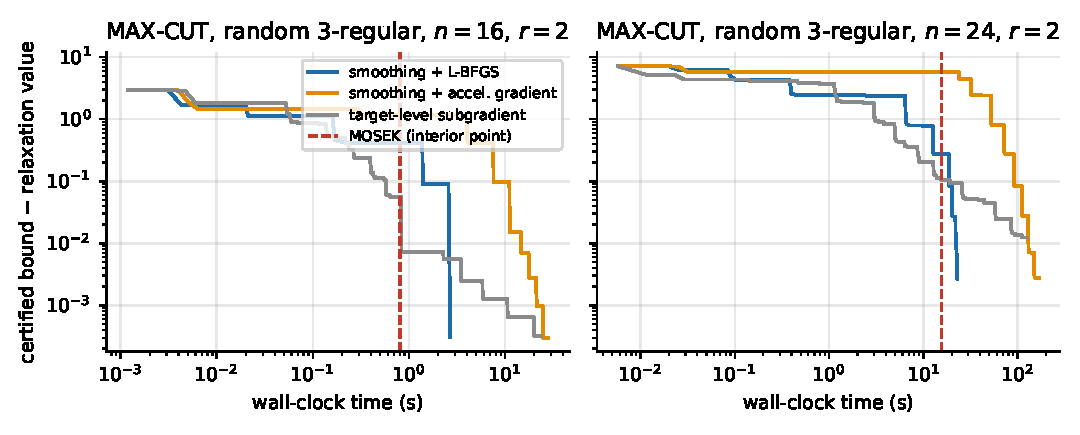
\includegraphics[width=\textwidth]{figures/convergence.pdf}
\caption{Certified bound minus the relaxation value (computed by MOSEK) against wall-clock time. Random $3$-regular graphs, one seed per size.}\label{fig:conv}
\end{figure}
\begin{table}[t]\centering\small
\begin{tabular}{r r c c c c}\toprule
$n$ & gap & L-BFGS & accel.\ grad. & subgradient & MOSEK (total) \\\midrule
16 & $10^{-1}$ & 1.39 & 7.57 & 0.57 & 0.8 \\
 & $10^{-2}$ & 2.58 & 14.59 & 0.83 &  \\
 & $10^{-3}$ & 2.65 & 21.13 & 10.57 &  \\
24 & $10^{-1}$ & 18.65 & 91.35 & 18.97 & 15.7 \\
 & $10^{-2}$ & 21.98 & 130 & -- &  \\
 & $10^{-3}$ & -- & -- & -- &  \\
\bottomrule\end{tabular}

\caption{Time (s) to reach a given gap above the exact relaxation value (``--'': not reached within the budget: $2\times10^4$ iterations for the subgradient method, $240$\,s for accelerated gradient, $\approx2\,000$ evaluations for L-BFGS).}\label{tab:e2}
\end{table}
Two observations deserve to be stated plainly. First, \emph{the plain subgradient method is better than its $O(1/\varepsilon^2)$ worst-case rate suggests}: with the Gram parametrization it reaches a gap of $10^{-2}$ in $0.8$\,s at $n=16$, faster than L-BFGS. It stalls however at high accuracy: it needs $10.6$\,s for $10^{-3}$ at $n=16$ (L-BFGS: $2.7$\,s) and does not reach $10^{-2}$ at $n=24$ within $2\times10^4$ iterations (L-BFGS: $22$\,s). Second, the accelerated-gradient scheme, which has the best worst-case complexity (\cref{thm:rate}), is the slowest in practice here; the theory is a worst-case guarantee, and L-BFGS exploits curvature far better. At $n=24$ no method reaches a gap of $10^{-3}$ within its budget, and MOSEK solves this size in $15.7$\,s, faster than any of the first-order solvers.

\subsection{Scaling in time and memory (E3)}\label{sec:scaling}
\Cref{tab:e3} and \cref{fig:scale} report order-$2$ MAX-CUT on random $3$-regular graphs from $n=10$ ($s=56$) to $n=60$ ($s=1831$, $1.68$ million multipliers).
\begin{table}[t]\centering\scriptsize
\setlength{\tabcolsep}{3pt}
\fitbox{\begin{tabular}{r r r r r r r r r r r}\toprule
$n$ & $s$ & \#mult. & $U$ (ours) & time & mem. & MOSEK value & time & mem. & best cut & $\lfloor U\rfloor$ \\\midrule
10 & 56 & 1{,}597 & 12.0002 & 0.5\,s & 0.13 & 12.0000 & 0.1\,s & 0.14 & 12 & 12 \\
14 & 106 & 5{,}672 & 19.0000 & 1.7\,s & 0.17 & 19.0000 & 0.4\,s & 0.21 & 19 & 19 \\
20 & 211 & 22{,}367 & 26.0010 & 8.7\,s & 0.21 & 26.0000 & 3.9\,s & 0.99 & 26 & 26 \\
26 & 352 & 62{,}129 & 36.0000 & 26.3\,s & 0.32 & 36.0000 & 43.0\,s & 5.41 & 36 & 36 \\
30 & 466 & 108{,}812 & 40.0026 & 61.6\,s & 0.44 & 40.0000 & 252.6\,s & 13.27 & 40 & 40 \\
40 & 821 & 337{,}432 & 54.0065 & 241.1\,s & 1.04 & \multicolumn{3}{c}{killed (SIGKILL; Schur matrix $\gtrsim$39\,GiB)} & 54 & 54 \\
50 & 1276 & 814{,}727 & 68.0040 & 582.7\,s & 1.89 & \multicolumn{3}{c}{not attempted} & 68 & 68 \\
60 & 1831 & 1{,}677{,}197 & 81.0195 & 2037.4\,s & 2.49 & \multicolumn{3}{c}{not attempted} & 81 & 81 \\
\bottomrule\end{tabular}
}
\caption{Order-$2$ MAX-CUT, random $3$-regular graphs. ``mem.'' is peak memory in GiB. ``Best cut'' is the best cut found by $2000$ restarts of single-flip local search (a feasible point), $\lfloor U\rfloor$ the bound of \cref{cor:integer}: when they agree the cut is \emph{certified optimal}. The MOSEK run at $n=40$ ($m=102{,}091$ constraints; Schur complement $\gtrsim39$\,GiB even with symmetric storage, on a $36$\,GiB machine) was terminated by the operating system (exit status~137); we infer out-of-memory from this and have not confirmed it by other means. MOSEK was not attempted for $n\ge50$.}\label{tab:e3}
\end{table}
\begin{figure}[t]\centering
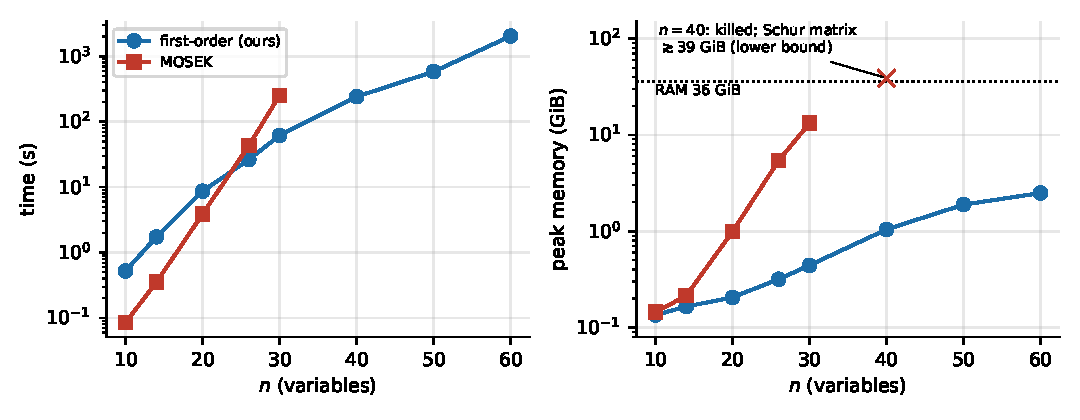
\includegraphics[width=\textwidth]{figures/scaling.pdf}
\caption{Time and peak memory of the first-order method and MOSEK. The cross marks a lower bound on the memory MOSEK would need at $n=40$.}\label{fig:scale}
\end{figure}
\begin{figure}[t]\centering
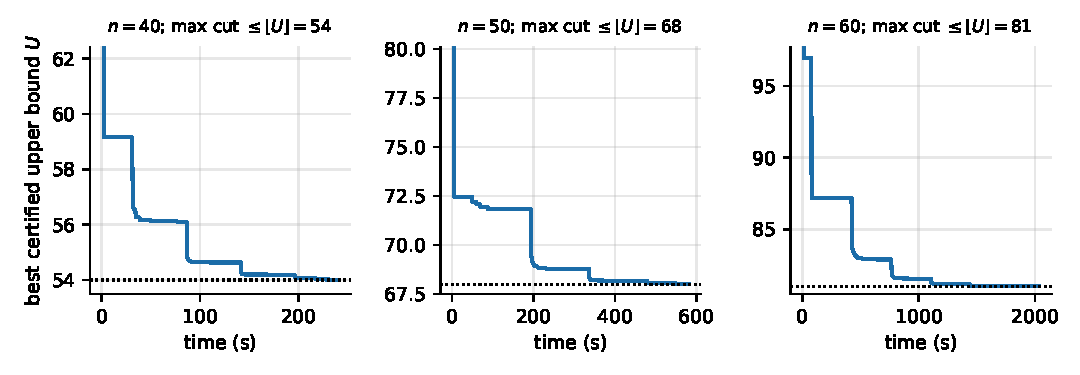
\includegraphics[width=\textwidth]{figures/anytime.pdf}
\caption{Anytime behaviour: best certified upper bound against time. Every point is a valid upper bound on the maximum cut; dotted: $\lfloor U\rfloor$ at the end of the run.}\label{fig:anytime}
\end{figure}
The picture is the following.
\begin{itemize}[leftmargin=1.5em]
\item \textbf{Time.} MOSEK is faster for $n\le20$ (e.g.\ $3.9$\,s versus $8.7$\,s at $n=20$). The curves cross near $n=26$; at $n=30$ the first-order method needs $62$\,s versus $253$\,s.
\item \textbf{Memory.} The memory of the first-order method grows from $0.13$ to $2.5$\,GiB over this range; MOSEK's grows from $0.14$ to $13.3$\,GiB at $n=30$ (a factor $30$ more than ours) and cannot be run at $n=40$.
\item \textbf{Accuracy.} The first-order values exceed the MOSEK values by at most $2.6\times10^{-3}$ ($n\le30$). For $n\ge40$ we have no interior-point reference.
\item \textbf{Certified optimality.} At every size the local-search cut equals $\lfloor U\rfloor$, so by \cref{cor:integer} \emph{the order-$2$ relaxation certifies that the best cut is the maximum cut}, for all graphs up to $n=60$. The margin between $U$ and the integer is $\le 0.02$ in all cases.
\item \textbf{Anytime.} \Cref{fig:anytime} shows the monotone decrease of the best certified bound; for $n=40$ the bound drops below $55$ after $\approx 120$\,s and below $54.01$ after $\approx 240$\,s, so a user who stops early still holds a valid certificate.
\end{itemize}
An earlier attempt at $n=60$ used a Lanczos eigensolver for blocks larger than $1500$; it did not converge within an hour and returned $87.2$, because at $s=1831$ a dense symmetric eigensolver ($0.4$\,s per call) is faster than ARPACK ($1.7$\,s). The reported numbers use the dense solver up to $s=2500$.

\subsection{Benchmark families from the Biq Mac distributions (E11)}\label{sec:bench}
So far all MAX-CUT instances were random $3$-regular graphs, a single family that is easy for order~$2$. \Cref{tab:bench} and \cref{fig:bench} report a benchmark of $60$ order-$2$ MAX-CUT instances drawn by seed from the distributions of the Biq Mac library~\cite{wiegele2007}: \texttt{g05} ($G(n,\tfrac12)$, unit weights), \texttt{pm1s} (density $0.1$, weights $\pm1$), \texttt{pm1d} (density $0.99$, weights $\pm1$) and a toroidal two-dimensional Ising grid with Gaussian weights $\times100$ rounded to integers, at three sizes each ($n=20,30,40$; $16,25,36$ for the grid) and five seeds per size (generators in \texttt{experiments/bench/instances.py}). They are \emph{not} the library instances (those require a download); only the distributions are the same. Every weight is an integer, so \cref{cor:integer} applies: the cut found by randomized single-flip local search ($2000$ restarts) is certified optimal as soon as $\lfloor U\rfloor$ equals it. We report $t_{\rm cert}$, the first time at which the best certified bound satisfies this, because it measures what the anytime property is worth in practice; the solver is the smoothing solver with the default schedule, run on the same machine in the same session with $8$ BLAS threads (load average at the start of a run: median $2.9$, maximum $10.7$; \cref{tab:bench} shows the median per row). The interior-point value (MOSEK) was computed for $n\le25$ only.
\begin{table}[t]\centering\scriptsize
\setlength{\tabcolsep}{3pt}
\fitbox{\begin{tabular}{l r r c r r r r r r}\toprule
family & $n$ & $s$ & cert./runs & $t_{\rm cert}$ med. [min,max] (s) & wall (s) & CPU (s) & mem.\ (GiB) & IPM wall (s) & load \\\midrule
g05 & 20 & 211 & 5/5 & 4.1 [3.8, 4.2] & 10.2 & 10.3 & 0.20 & 4.0 & 3 \\
pm1s & 20 & 211 & 5/5 & 3.1 [2.3, 3.2] & 9.4 & 9.5 & 0.20 & 3.8 & 3 \\
pm1d & 20 & 211 & 5/5 & 6.0 [5.9, 6.1] & 11.1 & 11.3 & 0.20 & 3.8 & 3 \\
torus & 16 & 137 & 5/5 & 1.2 [1.2, 1.3] & 1.6 & 1.6 & 0.15 & 0.8 & 2 \\
g05 & 30 & 466 & 5/5 & 22.2 [21.9, 23.8] & 57.7 & 58.4 & 0.45 & -- & 2 \\
pm1s & 30 & 466 & 5/5 & 32.5 [30.6, 33.5] & 74.2 & 74.9 & 0.46 & -- & 2 \\
pm1d & 30 & 466 & 5/5 & 33.3 [33.1, 50.3] & 68.0 & 68.7 & 0.46 & -- & 3 \\
torus & 25 & 326 & 5/5 & 15.0 [11.2, 20.2] & 16.3 & 16.4 & 0.27 & 28.0 & 6 \\
g05 & 40 & 821 & 5/5 & 126 [124, 186] & 239 & 242 & 1.11 & -- & 4 \\
pm1s & 40 & 821 & 5/5 & 111 [103, 114] & 253 & 257 & 1.12 & -- & 3 \\
pm1d & 40 & 821 & 5/5 & 165 [121, 167] & 240 & 244 & 1.11 & -- & 3 \\
torus & 36 & 667 & 5/5 & 71.0 [70.5, 83.1] & 81.0 & 81.8 & 0.78 & -- & 3 \\
\bottomrule\end{tabular}
}
\caption{Order-$2$ MAX-CUT on instances drawn from the Biq Mac distributions, five seeds per row. ``cert./runs'': runs whose best cut equals $\lfloor U\rfloor$ at the end; $t_{\rm cert}$: time until $\lfloor U\rfloor$ first equals the best cut (median, minimum and maximum over the seeds); wall and CPU: median total times of the run (smoothing schedule exhausted); ``IPM wall'': median wall-clock time of MOSEK on the same moment model ($n\le25$). ``load'': median load average at the start of the run (the machine is shared).}\label{tab:bench}
\end{table}
\begin{figure}[t]\centering
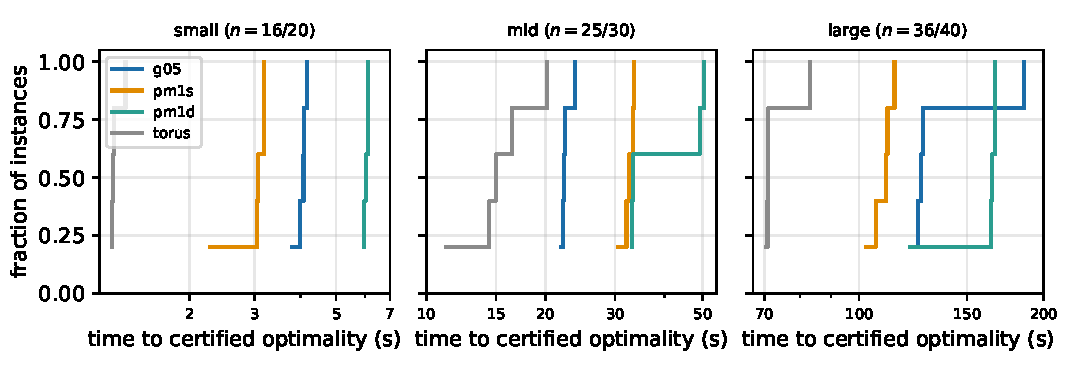
\includegraphics[width=\textwidth]{figures/bench_profile.pdf}
\caption{Fraction of instances whose optimality is certified within a given time, by family and size class.}\label{fig:bench}
\end{figure}
\emph{All $60$ instances are certified optimal}, with margins $U-\lfloor U\rfloor\le6.8\times10^{-3}$, and the value of the interior-point solver agrees with $\lfloor U\rfloor$ to $2.8\times10^{-6}$ on the $25$ instances where it was run. The time to certification is on median $0.50$ of the total time of the run (range $0.19$--$0.94$), so a user who stops at $t_{\rm cert}$ saves about half of the computation; it stays within $\pm20\%$ of the row median in $7$ of the $12$ rows (largest deviation $+51\%$) and grows by a factor $5.5$ from $n=20$ to $30$ and $5.7$ from $30$ to $40$ for \texttt{g05}, with at most $1.12$\,GiB of memory. Against the interior-point solver the picture is mixed, as in \cref{sec:scaling}: for $n\le25$ the time to certification is below MOSEK's total time in $10$ of $25$ runs (all five \texttt{pm1s} runs with $n=20$ and all five grid runs with $n=25$: $15$ against $28$\,s), equal on \texttt{g05} with $n=20$ ($4.1$ against $4.0$\,s) and larger on \texttt{pm1d} with $n=20$ ($6.0$ against $3.8$\,s) and on the grid with $n=16$ ($1.2$ against $0.8$\,s). The times in \cref{tab:bench} are those of the conservative default schedule; \cref{sec:e12} shows that a short schedule certifies about $20$ times faster. Two caveats apply. These families are easy at order~$2$ (the best cut was certified every time), so the benchmark shows consistency, not a stress test; and $t_{\rm cert}$ uses the floating-point certificate, whereas the rigorous verification of \cref{sec:e7} was run on the $3$-regular family only.

\paragraph{Real library instances.} We also ran five instances \texttt{g05\_60.0}--\texttt{g05\_60.4} ($n=60$, $885$ edges, unit weights) downloaded from the Biq Mac library~\cite{wiegele2007} (raw data \texttt{bench\_real.jsonl}); the larger library instances ($n=80,100$, and the Ising instances) exceed our dense order-$2$ model and were not run. The same default schedule as above certified the optimality of \emph{all five}: $\lfloor U\rfloor$ equals the best cut found by local search ($536$, $532$, $529$, $538$, $527$), after $794$--$1223$\,s (median $1102$\,s) out of $1440$--$1778$\,s in total, on a shared machine (load $1.6$--$6.1$). The optimal values were not compared with the library's published optima.

\subsection{Certification time: the smoothing schedule and low-rank starts (E12)}\label{sec:e12}
\Cref{sec:baselines} showed that Burer--Monteiro (BM) reaches primal accuracy faster than we do; but a \emph{bound} needs a dual point. We therefore compare four ways of obtaining a certified bound on the instances of \cref{sec:bench} (script \texttt{experiments/bench/hybrid\_cert.py}; all times include everything a pipeline does, and ``certified'' means $\lfloor U\rfloor$ equals the best cut, as before).
\begin{enumerate}[label=(\roman*),leftmargin=2em,nosep]
\item \emph{default schedule}: the smoothing solver of \cref{sec:bench}, $\eta=10^{-1},\dots,10^{-5}$;
\item \emph{short schedule}: the same solver started at $\theta=0$ with $\eta=10^{-3},3\cdot10^{-4},10^{-4},3\cdot10^{-5},10^{-5}$ ($n\le30$: five seeds per row; $n=36,40$: seeds $1,2$);
\item \emph{BM + multipliers}: the BM augmented Lagrangian of \cref{sec:baselines} ($k=10$, fixed $\beta=10$, $200$ inner L-BFGS iterations, chosen on three $n=20$ instances, not per instance) whose multiplier vector $z$ defines the dual slack matrix $S=D(-c+A^\top z)$, hence the dual point of our spectral dual with $U=\sum_iz_{{\rm diag},i}-s\,\lmin(S)$ (one eigenvalue computation per outer iteration; cap $100$\,s; run for $n\le30$ and not for $n\ge36$);
\item \emph{BM $\to$ refinement}: BM until its maximal constraint violation is $\le2\times10^{-3}$ (cap $60$\,s), then our solver from the dual point implied by $z$ with the short schedule.
\end{enumerate}
\begin{table}[t]\centering\scriptsize
\setlength{\tabcolsep}{3pt}
\fitbox{\begin{tabular}{l r r r r r r}\toprule
family & $n$ & default schedule & short schedule & BM + multipliers & BM $\to$ our refinement & BM phase (s)\\\midrule
g05 & 20 & 4.1 (5/5) & 0.1 (5/5) & 28.4 (5/5) & 2.3 (5/5) & 2.0 \\
g05 & 30 & 22.2 (5/5) & 0.9 (5/5) & -- (0/5) & 15.6 (5/5) & 12.5 \\
g05 & 40 & 126.3 (5/5) & 8.5 (5/5) & -- & 51.9 (5/5) & 27.9 \\
pm1s & 20 & 3.1 (5/5) & 0.1 (5/5) & 43.4 (4/5) & 1.6 (5/5) & 1.4 \\
pm1s & 30 & 32.5 (5/5) & 1.2 (5/5) & -- (0/5) & 9.6 (5/5) & 6.9 \\
pm1s & 40 & 110.8 (5/5) & 4.8 (5/5) & -- & 42.9 (5/5) & 33.3 \\
pm1d & 20 & 6.0 (5/5) & 0.2 (5/5) & 17.0 (5/5) & 1.9 (5/5) & 1.6 \\
pm1d & 30 & 33.3 (5/5) & 1.9 (5/5) & -- (0/5) & 14.3 (5/5) & 11.5 \\
pm1d & 40 & 164.5 (5/5) & 14.7 (5/5) & -- & 60.2 (5/5) & 39.0 \\
torus & 16 & 1.2 (5/5) & 1.4 (5/5) & 0.6 (5/5) & 0.7 (5/5) & 0.6 \\
torus & 25 & 15.0 (5/5) & 4.7 (5/5) & 7.0 (5/5) & 3.0 (5/5) & 2.9 \\
torus & 36 & 71.0 (5/5) & 36.7 (2/5) & -- & 55.0 (5/5) & 46.6 \\
reg3 & 50 & 201 (1/1) & 34 (5/5) & -- & -- & -- \\
reg3 & 60 & 766 (1/1) & 353 (3/3) & -- & -- & -- \\
\bottomrule\end{tabular}
}
\caption{Median time (s) to a certified optimal cut, with (certified runs / runs) in parentheses; ``--'' without parentheses: not run. The last column is the median time spent in the BM phase of (iv). The \texttt{reg3} rows are random $3$-regular graphs (five instances at $n=50$, three at $n=60$); their default-schedule entry is the single seed-$1$ instance of \cref{tab:e3}.}\label{tab:e12}
\end{table}
Four observations. \emph{(1) The schedule matters more than anything else, for unit and $\pm1$ weights.} The short schedule is faster than the default one by a median factor $20.0$ over the $57$ paired runs in which both certified (range $0.6$--$60.5$); by size the median factor is $31.6$, $23.5$ and $13.6$ at $n=20,30,40$ for the three random-graph families, but only $0.9$, $2.4$ and $2.1$ on the grid. On \texttt{g05}, $n=30$, it certifies in $0.9$\,s instead of $22$\,s; a direct check at $n=20$ and $n=30$ with independent re-evaluation of the certificate gave $38$ and $19$ function evaluations instead of $732$ and $711$. The reason is that integer optimality needs only $U<\text{best cut}+1$, so the first, coarse smoothing stages ($\eta\ge10^{-2}$) are unnecessary; the schedule of \cref{sec:algo} is appropriate for accuracy ($10^{-3}$ above the relaxation value) but not for certification. The short schedule certified $57$ of the $60$ runs; the three failures are all on the grid with $n=36$ (seeds $1,3,5$; final $U-{\rm best\ cut}=4.8,\ 7.9,\ 1.6$), where the weights are of order $100$ and the required relative accuracy is ten times higher; the default schedule certified all five. A rerun of these three with $2000$ instead of $500$ iterations per stage and two further stages ($\eta$ down to $10^{-6}$) certified all of them after $61$--$79$\,s with final gap $0.00$ (\texttt{experiments/results/torus\_fix.txt}), so the failures reflect the cap on iterations per stage rather than the choice of $\eta$. On random $3$-regular graphs (\texttt{reg3} rows) the short schedule certified all five instances at $n=50$ (median $34$\,s, range $12$--$149$\,s) and all three at $n=60$ ($352$--$358$\,s, each close to the end of the first stage of $500$ iterations on a $1831\times1831$ block; a single earlier run with $300$ iterations per stage needed $218$\,s), against $201$\,s and $766$\,s for the default schedule on the seed-$1$ instance, i.e.\ factors $5.9$ and $2.1$ for that instance (the default-schedule runs of \cref{sec:scaling} were made under a different load; the short runs under a load average of about $3$--$4$; \texttt{experiments/results/cold\_large.txt}, \texttt{bench\_hybrid.jsonl}).
\emph{(2) The BM multipliers are a poor dual point.} The primal value of BM is accurate to $10^{-3}$ within seconds, but its multiplier estimate is not: with $\beta$ increasing, as in \cref{sec:baselines}, $U$ grows from $76$ to above $130$ on a $n=20$ instance whose optimum is $71$; with fixed $\beta$ the certificate improves slowly. BM + multipliers certified $19$ of $20$ runs for $n=16,20$ (median $17$--$43$\,s on the random graphs) and \emph{none} of the $15$ random-graph runs with $n=30$ within $100$\,s, while the short schedule needs $0.9$--$1.9$\,s. On the grid family, BM + multipliers is competitive ($0.6$\,s at $n=16$ and $7.0$\,s at $n=25$, against $1.4$\,s and $4.7$\,s for the short schedule).
\emph{(3) A low-rank start does not help in general.} BM $\to$ refinement certifies all $60$ runs and is faster than the default schedule everywhere ($1.3$--$5\times$), which first suggested a benefit of the low-rank start; but compared with the short schedule at $\theta=0$ it is faster in only $11$ of the $57$ paired runs, because the BM phase ($70$--$95\%$ of its time) costs more than the coarse stages it saves. It is competitive only on the grid ($3.0$ against $4.7$\,s at $n=25$).
\emph{(4) What this changes.} The times of \cref{sec:scaling,sec:bench} (default schedule, run to $10^{-3}$ accuracy) are conservative for the purpose of \emph{certifying optimality} when the weights are $0/1$ or $\pm1$: by a factor of about $14$--$32$ at $n\le40$ and $2$--$6$ at $n=50,60$; for the weighted grid they are not. They remain the right numbers for the relaxation \emph{value} to $10^{-3}$, for which the full schedule is needed. We have not examined whether a coarse start is as effective outside constant-trace Boolean problems.

\emph{Additional results} on higher relaxation orders ($r=3$, $n=20,24$), on correlative sparsity and on non-convex box QPs are in \cref{app:extra}.

\subsection{Other first-order solvers (E6)}\label{sec:baselines}
We also compared with three other first-order approaches on the same order-$2$ MAX-CUT relaxations ($n=16,\dots,40$): SCS~\cite{odonoghue2016} (ADMM, through CVXPY on the same moment model), a dense conditional-gradient augmented-Lagrangian method (CGAL, \cite{yurtsever2021} without the sketch) and a Burer--Monteiro augmented Lagrangian~\cite{burer2003} with $L$-BFGS-B inner solves ($k=8,16$). These experiments were run by a separate script set under \texttt{experiments/baselines/}. The baselines' parameters ($\beta_0$, $k$) were tuned \emph{per instance using the reference value}, which favours them; our method was not tuned per instance. Since CGAL, Burer--Monteiro and SCS return values of infeasible or inexact iterates, ``reaching accuracy $10^{-3}$'' for them means $|{\rm value}-{\rm ref}|\le10^{-3}$ \emph{and} constraint violation $\le10^{-3}$; ours is a certified upper bound minus the reference.
\begin{figure}[t]\centering
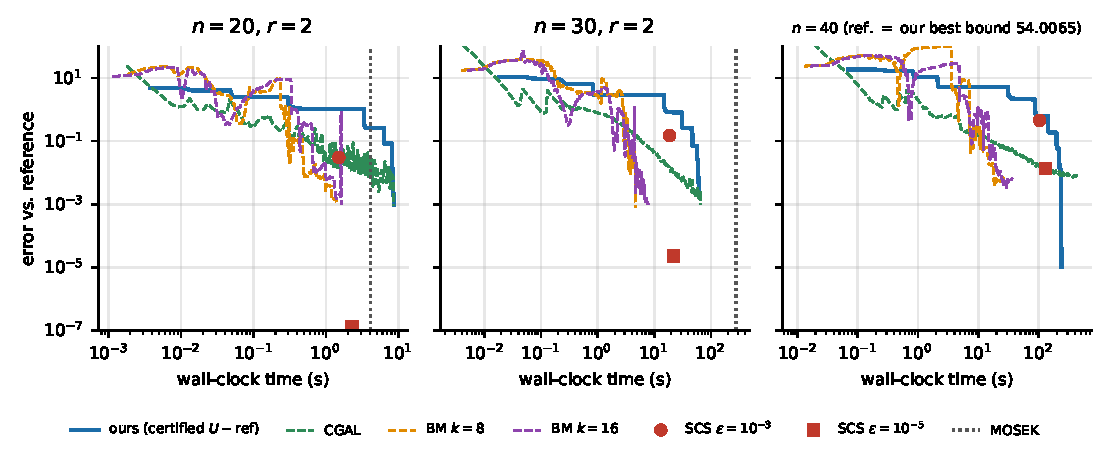
\includegraphics[width=\textwidth]{figures/baselines.pdf}
\caption{Error against time for our certified method and other first-order solvers on order-$2$ MAX-CUT (panels $n=20,30,40$). Only ours is a rigorous upper bound at every point.}\label{fig:baselines}
\end{figure}
The outcome is unfavourable to our method in speed: \emph{at every size at least one non-certified baseline reaches $10^{-3}$ faster than we do, and Burer--Monteiro is the fastest} (e.g.\ $n=30$: $4.7$\,s for $k=8$ versus $62$\,s for ours, which reaches only $2.6\times10^{-3}$; at $n=40$ against the reference $54.0065$ none of the baselines reaches $10^{-3}$ with feasibility, but against the integer $54$ Burer--Monteiro needs about $26$--$37$\,s). SCS with $\varepsilon=10^{-5}$ is also faster for $n\le30$, but with $\varepsilon=10^{-3}$ its error is $2\times10^{-3}$--$0.45$, i.e.\ unreliable; its memory is up to $1.1$\,GiB at $n=40$ (ours $1.0$\,GiB). All first-order methods beat MOSEK from $n\ge26$ in time and memory. (Their primal accuracy is not their certificate time: \cref{sec:e12} builds a bound from BM's multipliers and finds it slower than our solver.) TSSOS~\cite{magron2021tssos} (Julia $1.13.3$, MOSEK as SDP solver, dense order-$2$ Boolean relaxation \texttt{cs\_tssos(..., nb=n, CS=false)}) returns the same values as the interior-point reference on the instances $n=10,14,20,26,30$ (e.g.\ $40.0000$ at $n=30$) and is thus not an independent first-order competitor but an interior-point one: its times ($12$, $12$, $16$, $58$, $264$\,s, each including about $12$\,s of Julia start-up and compilation) follow those of MOSEK on the same model ($0.1$, $0.4$, $3.9$, $43$, $253$\,s), and are slower than ours from $n=26$ ($26$\,s) and $n=30$ ($62$\,s). On these dense graphs correlative sparsity does not apply (one clique), so CS-TSSOS reduces to the same dense relaxation. What the baselines do not provide is a bound: they return primal values with constraint violation about $10^{-3}$, whereas every iterate of ours is a certified upper bound (\cref{thm:certificate}); the price of certification, in our experiments, is a factor $5$--$15$ in time at $n\ge20$ compared with the best heuristic (\cref{tab:baselines} in the appendix).

\subsection{Augmented Lagrangian on MAX-CUT and instance variability (E10)}\label{sec:e10}
\paragraph{ALM on MAX-CUT.} The dual augmented Lagrangian of \cref{sec:alm} was so far used only on the neural-network problems. \Cref{tab:e10a} and \cref{fig:alm} compare it (NumPy port \texttt{msos.solvers.alm}, validated against \texttt{moment\_sos.solve\_alm} and the interior-point value on Petersen and disk to $10^{-6}$) with the smoothing solver on order-$2$ MAX-CUT, $n=16$--$30$, for $\rho_0\in\{100,300,1000\}$, with a budget of $600$\,s ($900$\,s at $n=30$). The reference is the integer maximum cut ($22,26,32,40$), which equals $\rho_2$ on these graphs (Clarabel at $n=16$; the certified bounds themselves at $n\ge20$, where $\min U-\lfloor U\rfloor\le6\times10^{-8}$). Script \texttt{e10a\_alm\_maxcut.py}.
\begin{table}[t]\centering\scriptsize
\setlength{\tabcolsep}{3pt}
\fitbox{\begin{tabular}{r l c c c c c r r}\toprule
$n$ & solver & $t_{10^{-1}}$ & $t_{10^{-2}}$ & $t_{10^{-3}}$ & $t_{10^{-4}}$ & final gap & wall (s) & CPU (s) \\\midrule
16 & smoothing + L-BFGS & 16.6 & 28.0 & 29.0 & -- & $3.1\times10^{-4}$ & 29 & 12 \\
 & ALM, $\rho_0=100$ & 60.3 & 62.7 & 62.7 & 62.7 & $1.0\times10^{-10}$ & 65 & 52 \\
 & ALM, $\rho_0=300$ & 70.2 & 70.5 & 70.5 & 70.5 & $5.0\times10^{-9}$ & 71 & 38 \\
 & ALM, $\rho_0=1000$ & 20.2 & 20.2 & 20.2 & 20.2 & $3.7\times10^{-11}$ & 20 & 22 \\
\addlinespace
20 & smoothing + L-BFGS & 38.0 & 56.9 & 58.6 & -- & $9.6\times10^{-4}$ & 60 & 42 \\
 & ALM, $\rho_0=100$ & 221 & 221 & 221 & 221 & $2.6\times10^{-9}$ & 228 & 155 \\
 & ALM, $\rho_0=300$ & 149 & 149 & 153 & 153 & $6.7\times10^{-8}$ & 157 & 126 \\
 & ALM, $\rho_0=1000$ & 89.7 & 91.1 & 91.1 & 91.1 & $2.6\times10^{-8}$ & 93 & 88 \\
\addlinespace
24 & smoothing + L-BFGS & 42.9 & 50.5 & -- & -- & $2.7\times10^{-3}$ & 53 & 69 \\
 & ALM, $\rho_0=100$ & 213 & 230 & 230 & 230 & $5.3\times10^{-8}$ & 249 & 325 \\
 & ALM, $\rho_0=300$ & 240 & 258 & 258 & 259 & $1.0\times10^{-8}$ & 280 & 319 \\
 & ALM, $\rho_0=1000$ & 273 & 273 & 274 & 274 & $1.5\times10^{-8}$ & 314 & 265 \\
\addlinespace
30 & smoothing + L-BFGS & 151 & 170 & -- & -- & $2.6\times10^{-3}$ & 175 & 190 \\
 & ALM, $\rho_0=100$ & -- & -- & -- & -- & $3.1\times10^{-1}$ & 910 & 915 \\
 & ALM, $\rho_0=300$ & -- & -- & -- & -- & $4.9\times10^{-1}$ & 950 & 769 \\
 & ALM, $\rho_0=1000$ & 574 & 575 & 577 & 583 & $1.6\times10^{-8}$ & 600 & 756 \\
\bottomrule\end{tabular}
}
\caption{Order-$2$ MAX-CUT, random $3$-regular graphs (seed $1$): wall-clock time (s) to a \emph{certified} gap $U-\rho_2\le10^{-k}$ (``--'': not reached), final gap, wall and CPU time. ALM evaluates the certificate at every outer iterate and every $20$ inner evaluations. Shared machine (load $13$--$94$ on $14$ cores during the runs), $3$ BLAS threads per run: wall times are inflated and noisy, CPU times are the more robust column.}\label{tab:e10a}
\end{table}
\begin{figure}[t]\centering
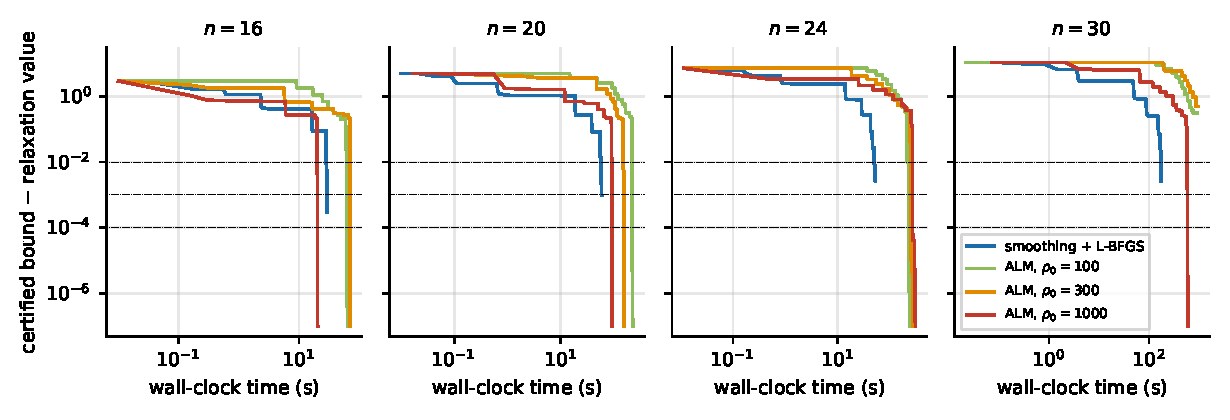
\includegraphics[width=\textwidth]{figures/alm_maxcut.pdf}
\caption{Certified gap against time for the smoothing solver and the dual augmented Lagrangian on order-$2$ MAX-CUT.}\label{fig:alm}
\end{figure}
The outcome qualifies the moderate accuracy of the smoothing solver noted in \cref{sec:disc}: it is not intrinsic to the oracle. \emph{The augmented Lagrangian reaches gaps between $4\times10^{-11}$ and $7\times10^{-8}$}---i.e.\ the relaxation value to essentially interior-point accuracy, with a certificate---on every instance for which it converges, whereas the smoothing solver stalls at $3\times10^{-4}$--$3\times10^{-3}$ with the default schedule. Its behaviour is a plateau followed by a collapse of the gap by eight orders of magnitude within one or two outer iterations (\cref{fig:alm}), so the time to $10^{-4}$ is essentially the time to $10^{-1}$. The smoothing solver remains the better \emph{anytime} method at low accuracy ($10^{-1}$ in $17$--$151$\,s against $20$--$574$\,s for the best ALM run), and at $n=20$ it reaches $10^{-3}$ first ($59$\,s against $91$\,s). The penalty parameter matters as in \cref{sec:alm}: $\rho_0=1000$ is the fastest at $n=16,20,30$ and the only setting that converges at $n=30$ within $900$\,s ($584$\,s; $\rho_0=100,300$ end at gaps $0.3$--$0.5$), while at $n=24$ all three converge in $230$--$274$\,s. We therefore keep $\rho_0=1000$ as the default and recommend the ALM whenever the relaxation value itself, rather than an early bound, is wanted; the peak memory of the two solvers is comparable ($0.2$--$0.4$\,GiB for smoothing, $0.2$--$0.6$\,GiB for ALM).

\paragraph{Instance variability.} \Cref{tab:e10b} addresses limitation~(4): five random $3$-regular graphs per size (seeds $1$--$5$) at $n=16,20,24$, solved with the smoothing solver at the paper's settings, with the maximum cut by exhaustive enumeration (script \texttt{e10b\_variability.py}).
\begin{table}[t]\centering\small
\fitbox{\begin{tabular}{r r r l l l c c}\toprule
$n$ & $s$ & inst. & wall time (s) & CPU time (s) & margin $U-\lfloor U\rfloor$ & certified & IPM wall (s) \\\midrule
16 & 137 & 5 & 9.8 [7.5, 15.2] & 9.8 [8.4, 11.7] & 4.7e-04 [3.1e-04, 1.0e-03] & 5/5 & 45.6 \\
20 & 211 & 5 & 41.4 [18.5, 119.7] & 31.5 [23.3, 48.1] & 1.0e-03 [3.7e-04, 1.8e-03] & 5/5 & 1204.7 (1/5) \\
24 & 301 & 5 & 60.6 [51.7, 72.1] & 72.3 [66.0, 80.0] & 2.3e-03 [1.3e-03, 2.7e-03] & 5/5 & -- \\
\bottomrule\end{tabular}
}
\caption{Variability over five random $3$-regular graphs per size (mean [min, max]). ``certified'': instances with $\lfloor U\rfloor=$ maximum cut. ``IPM'': Clarabel on the moment model (at $n=20$ only one of five instances finished within the $600$\,s cap; not attempted at $n=24$). CPU time at $n=16$ from a re-timed run.}\label{tab:e10b}
\end{table}
All $15$ instances are certified optimal through the order-$2$ relaxation ($\lfloor U\rfloor$ equals the maximum cut), with margins $U-\lfloor U\rfloor$ between $3\times10^{-4}$ and $2.7\times10^{-3}$ and the interior-point value rounding to the cut wherever it was computed. The spread over instances is moderate at $n=16$ and $24$ (wall time within a factor $2$, evaluations within $\pm25\%$) and large at $n=20$ ($18$--$120$\,s), where the CPU times ($23$--$48$\,s) show that most of the spread is machine load rather than instance difficulty. The conclusions of \cref{sec:exp} drawn from the seed-$1$ instances are thus representative for this graph family, within a factor of about $2$ in time.

\section{Validation of the certificates, primal recovery and cuts}\label{sec:validation}
The following experiments check the statements of \cref{sec:rigor,sec:primal} and \cref{prop:diag} on the MAX-CUT and POP instances of \cref{sec:exp}.
\subsection{Rigorous certificates (E7)}\label{sec:e7}
\Cref{tab:e7} applies \cref{thm:rigor} to the floating-point output of the smoothing solver on the $23$ instances of \cref{tab:e1} and on order-$2$ MAX-CUT on the random $3$-regular graphs of \cref{tab:e3} for $n=10$--$40$ (script \texttt{e7\_rigor.py}, module \texttt{msos/verify.py}). The verified eigenvalue bound of \cref{lem:chol} is obtained with the column-oriented Cholesky factorization of $\hat Q_b+\alpha I$, $\alpha=-\hat\ell_b+\epsilon$ with the initial margin $\epsilon=\max(10^{-12},10^{-10}|\hat\ell_b|,64u\|\hat Q_b\|_F)$; it succeeded on every block without a single doubling of $\epsilon$. The exact residual $E$ of the Gram identity is computed in integer arithmetic after scaling by a common power of two.
\begin{table}[t]\centering\scriptsize
\setlength{\tabcolsep}{3pt}
\fitbox{\begin{tabular}{l c r r r r r r r c}\toprule
Problem & $r$ & $s$ & $U$ & $U_{\rm rig}-U$ & $E$ & max eig.\ slack & $t_{\rm chol}$ [s] & $t_{\rm res}$ [s] & certified? \\\midrule
ball & 2 & 3 & 1.000000 & $3.0\times10^{-11}$ & $1.3\times10^{-14}$ & $1.0\times10^{-11}$ & 0.000 & 0.000 & -- \\
disk & 2 & 6 & 1.414217 & $6.0\times10^{-13}$ & $6.0\times10^{-13}$ & $3.5\times10^{-11}$ & 0.000 & 0.000 & -- \\
sphere (eq.) & 2 & 6 & 1.414214 & $4.0\times10^{-14}$ & $4.0\times10^{-14}$ & $1.0\times10^{-12}$ & 0.000 & 0.000 & -- \\
MAX-CUT K3 & 1 & 4 & 2.250003 & $2.3\times10^{-10}$ & $9.5\times10^{-18}$ & $5.6\times10^{-11}$ & 0.000 & 0.000 & yes ($\lfloor U_{\rm rig}\rfloor=2$) \\
MAX-CUT K3 & 2 & 7 & 2.000004 & $2.0\times10^{-10}$ & $1.1\times10^{-15}$ & $2.9\times10^{-11}$ & 0.000 & 0.000 & yes ($\lfloor U_{\rm rig}\rfloor=2$) \\
MAX-CUT K3 & 3 & 8 & 2.000000 & $2.0\times10^{-10}$ & 0 & $2.5\times10^{-11}$ & 0.000 & 0.000 & yes ($\lfloor U_{\rm rig}\rfloor=2$) \\
MAX-CUT C5 & 1 & 6 & 4.522545 & $4.5\times10^{-10}$ & $6.5\times10^{-16}$ & $7.5\times10^{-11}$ & 0.000 & 0.000 & yes ($\lfloor U_{\rm rig}\rfloor=4$) \\
MAX-CUT C5 & 2 & 16 & 4.000053 & $4.0\times10^{-10}$ & $8.3\times10^{-14}$ & $2.5\times10^{-11}$ & 0.000 & 0.000 & yes ($\lfloor U_{\rm rig}\rfloor=4$) \\
MAX-CUT C5 & 3 & 26 & 4.000034 & $4.0\times10^{-10}$ & $1.2\times10^{-14}$ & $1.5\times10^{-11}$ & 0.000 & 0.000 & yes ($\lfloor U_{\rm rig}\rfloor=4$) \\
MAX-CUT K5 & 1 & 6 & 6.250002 & $6.3\times10^{-10}$ & $2.4\times10^{-16}$ & $1.0\times10^{-10}$ & 0.000 & 0.000 & yes ($\lfloor U_{\rm rig}\rfloor=6$) \\
MAX-CUT K5 & 2 & 16 & 6.250021 & $6.3\times10^{-10}$ & $2.2\times10^{-14}$ & $3.9\times10^{-11}$ & 0.000 & 0.000 & yes ($\lfloor U_{\rm rig}\rfloor=6$) \\
MAX-CUT K5 & 3 & 26 & 6.000032 & $6.0\times10^{-10}$ & $3.3\times10^{-14}$ & $2.3\times10^{-11}$ & 0.000 & 0.000 & yes ($\lfloor U_{\rm rig}\rfloor=6$) \\
MAX-CUT Petersen & 1 & 11 & 12.500009 & $1.3\times10^{-9}$ & $7.5\times10^{-16}$ & $1.1\times10^{-10}$ & 0.000 & 0.000 & yes ($\lfloor U_{\rm rig}\rfloor=12$) \\
MAX-CUT Petersen & 2 & 56 & 12.000124 & $1.2\times10^{-9}$ & $2.5\times10^{-12}$ & $2.1\times10^{-11}$ & 0.000 & 0.000 & yes ($\lfloor U_{\rm rig}\rfloor=12$) \\
MAX-CUT K7 & 1 & 8 & 12.250001 & $1.2\times10^{-9}$ & $2.7\times10^{-15}$ & $1.5\times10^{-10}$ & 0.000 & 0.000 & yes ($\lfloor U_{\rm rig}\rfloor=12$) \\
MAX-CUT K7 & 2 & 29 & 12.250021 & $1.2\times10^{-9}$ & $1.1\times10^{-13}$ & $4.2\times10^{-11}$ & 0.000 & 0.000 & yes ($\lfloor U_{\rm rig}\rfloor=12$) \\
MAX-CUT K7 & 3 & 64 & 12.250100 & $1.2\times10^{-9}$ & $1.4\times10^{-13}$ & $1.9\times10^{-11}$ & 0.000 & 0.001 & yes ($\lfloor U_{\rm rig}\rfloor=12$) \\
MAX-CUT reg3-12 & 1 & 13 & 16.000005 & $1.6\times10^{-9}$ & $2.1\times10^{-14}$ & $1.2\times10^{-10}$ & 0.000 & 0.000 & yes ($\lfloor U_{\rm rig}\rfloor=16$) \\
MAX-CUT reg3-12 & 2 & 79 & 16.000102 & $1.6\times10^{-9}$ & $3.6\times10^{-12}$ & $2.0\times10^{-11}$ & 0.000 & 0.001 & yes ($\lfloor U_{\rm rig}\rfloor=16$) \\
box QP n=5 (seed 1) & 2 & 21 & 8.611096 & $2.9\times10^{-11}$ & $1.5\times10^{-12}$ & $3.9\times10^{-11}$ & 0.000 & 0.000 & -- \\
box QP n=5 (seed 2) & 2 & 21 & 10.852148 & $2.8\times10^{-11}$ & $5.9\times10^{-12}$ & $3.5\times10^{-11}$ & 0.000 & 0.000 & -- \\
chain quartic n=8 (sparse) & 2 & 6 & 2.014187 & $5.2\times10^{-11}$ & $7.4\times10^{-13}$ & $1.4\times10^{-11}$ & 0.001 & 0.000 & -- \\
chain quartic n=8 (dense) & 2 & 45 & 2.014266 & $6.6\times10^{-11}$ & $9.7\times10^{-13}$ & $3.5\times10^{-12}$ & 0.001 & 0.001 & -- \\
MAX-CUT reg3 n=10 & 2 & 56 & 12.000174 & $1.2\times10^{-9}$ & $1.2\times10^{-12}$ & $2.1\times10^{-11}$ & 0.000 & 0.000 & yes ($\lfloor U_{\rm rig}\rfloor=12$) \\
MAX-CUT reg3 n=14 & 2 & 106 & 19.000019 & $1.9\times10^{-9}$ & $4.1\times10^{-12}$ & $1.8\times10^{-11}$ & 0.001 & 0.001 & yes ($\lfloor U_{\rm rig}\rfloor=19$) \\
MAX-CUT reg3 n=20 & 2 & 211 & 26.000957 & $2.7\times10^{-9}$ & $5.0\times10^{-12}$ & $1.3\times10^{-11}$ & 0.002 & 0.005 & yes ($\lfloor U_{\rm rig}\rfloor=26$) \\
MAX-CUT reg3 n=26 & 2 & 352 & 36.000032 & $3.8\times10^{-9}$ & $1.0\times10^{-11}$ & $1.1\times10^{-11}$ & 0.006 & 0.016 & yes ($\lfloor U_{\rm rig}\rfloor=36$) \\
MAX-CUT reg3 n=30 & 2 & 466 & 40.002593 & $4.4\times10^{-9}$ & $9.7\times10^{-12}$ & $9.5\times10^{-12}$ & 0.12 & 0.10 & yes ($\lfloor U_{\rm rig}\rfloor=40$) \\
MAX-CUT reg3 n=40 & 2 & 821 & 54.006422 & $7.2\times10^{-9}$ & $1.8\times10^{-11}$ & $8.8\times10^{-12}$ & 0.068 & 0.14 & yes ($\lfloor U_{\rm rig}\rfloor=54$) \\
\bottomrule\end{tabular}
}
\caption{Rigorous a posteriori certificates (\cref{thm:rigor}). $U$ is the floating-point certificate, $U_{\rm rig}-U$ the rigorous correction, $E$ the exact residual of \eqref{eq:identity}, ``max eig.\ slack'' the largest $\hat\ell_b-\ell_b$ over the blocks, $t_{\rm chol}$ and $t_{\rm res}$ the times of the Cholesky verification and of the exact residual. For MAX-CUT, ``certified'' means $\lfloor U_{\rm rig}\rfloor=\lfloor U\rfloor=$ best cut.}\label{tab:e7}
\end{table}
On all $29$ rows $U_{\rm rig}\ge U$, and the correction $U_{\rm rig}-U$ lies between $4\times10^{-14}$ (sphere) and $7.2\times10^{-9}$ (MAX-CUT $n=40$, $s=821$). It is dominated not by the backward-error term $\gamma_{s+1}\|\hat R\|_F^2$ (below $10^{-11}$ even at $s=821$) but by the deliberately chosen margin $10^{-10}|\hat\ell_b|$ multiplied by the block weight $s_k$: for the Boolean rows $U_{\rm rig}-U\approx10^{-10}(U-\sigma)$. The exact residual is $E\le1.8\times10^{-11}$ (median $10^{-13}$); it reflects the drift of the zero-sum variables and of the floating-point assembly of $\hat Q_b$ over thousands of iterations. The cost is negligible: at $s=821$ ($102{,}091$ moments, $337{,}000$ slots) the Cholesky verification takes $0.07$\,s and the exact residual $0.14$\,s in Python integers, against $559$\,s for the solve. In all $22$ MAX-CUT rows $\lfloor U_{\rm rig}\rfloor=\lfloor U\rfloor$ equals the best cut, so the optimality certificates of \cref{tab:e3} for $n\le40$ hold in exact arithmetic (for the floating-point MAX-CUT data $\pm\tfrac12$, which are exact).

\subsection{Primal recovery and two-sided certificates (E8)}\label{sec:e8}
\Cref{tab:e8} and \cref{fig:primal} evaluate \cref{prop:primal} along the default $\eta$-continuation (script \texttt{e8\_primal.py}; every oracle call also returns $\bar y$, $L_{\bar y}(f)$, the lower bound LB of part (d) and the infeasibility measures of part (b)). The reference $\rho_2$ is computed by Clarabel for $n=12,16$ and the non-Boolean problems; for $n=20,24,30$ it is the integer maximum cut ($26,32,40$; exact by enumeration for $n\le24$), which the bracket of part (d) itself confirms to be $\rho_2$ up to the final $U-\rho_2$ column.
\begin{table}[t]\centering\scriptsize
\setlength{\tabcolsep}{3pt}
\fitbox{\begin{tabular}{r r r r r r r r r r}\toprule
$n$ & $s$ & $\rho_2$ & $U-\rho_2$ & $\rho_2-{\rm LB}$ & $|L_{\bar y}(f)-\rho_2|$ & $t_{10^{-2}}$ & $t_{10^{-3}}$ & $t^{U}_{10^{-3}}$ & $t^{L}_{10^{-3}}$ \\\midrule
12 & 79 & 16.00000 & $1.0\cdot10^{-4}$ & $4.4\cdot10^{-3}$ & $8.8\cdot10^{-4}$ & 2.37 & -- & 2.41 & 1.31 \\
16 & 137 & 22.00000 & $3.1\cdot10^{-4}$ & $8.0\cdot10^{-3}$ & $5.2\cdot10^{-4}$ & 10.6 & -- & 10.5 & 10.3 \\
20 & 211 & 26.00000$^\dagger$ & $9.6\cdot10^{-4}$ & $3.5\cdot10^{-2}$ & $2.8\cdot10^{-4}$ & -- & -- & 32.0 & 29.4 \\
24 & 301 & 32.00000$^\dagger$ & $2.7\cdot10^{-3}$ & $4.6\cdot10^{-2}$ & $2.5\cdot10^{-4}$ & -- & -- & -- & 172 \\
30 & 466 & 40.00000$^\dagger$ & $2.6\cdot10^{-3}$ & $7.7\cdot10^{-2}$ & $1.1\cdot10^{-3}$ & -- & -- & -- & 297 \\
\midrule
\multicolumn{10}{l}{\footnotesize non-Boolean, $r=2$ (no lower bound): problem, $\rho_2^{\rm tr}$, $U-\rho^{\rm tr}_2$, $L_{\bar y}(f)-\rho^{\rm tr}_2$ (final / best stage), infeasibility, $\|g\|$} \\
\midrule
\multicolumn{2}{l}{box QP $n{=}5$ (seed 1)} & 8.61100 & $9.6\cdot10^{-5}$ & \multicolumn{2}{c}{$+9.6\cdot10^{-3}$ / $-1.6\cdot10^{-6}$ ($\eta{=}10^{-2}$)} & \multicolumn{2}{c}{$4.1\cdot10^{-2}$} & \multicolumn{2}{c}{$2.4\cdot10^{-2}$} \\
\multicolumn{2}{l}{box QP $n{=}5$ (seed 2)} & 10.85204 & $1.1\cdot10^{-4}$ & \multicolumn{2}{c}{$+5.7\cdot10^{-3}$ / $-1.5\cdot10^{-4}$ ($\eta{=}10^{-3}$)} & \multicolumn{2}{c}{$2.1\cdot10^{-2}$} & \multicolumn{2}{c}{$1.1\cdot10^{-2}$} \\
\multicolumn{2}{l}{chain quartic $n{=}8$ (sparse)} & 2.01404 & $1.4\cdot10^{-4}$ & \multicolumn{2}{c}{$+1.5\cdot10^{-4}$ / $+1.0\cdot10^{-4}$ ($\eta{=}10^{-4}$)} & \multicolumn{2}{c}{$2.3\cdot10^{-2}$} & \multicolumn{2}{c}{$1.2\cdot10^{-2}$} \\
\multicolumn{2}{l}{disk} & 1.41421 & $3.7\cdot10^{-6}$ & \multicolumn{2}{c}{$-2.3\cdot10^{-4}$ / $-1.7\cdot10^{-6}$ ($\eta{=}10^{-2}$)} & \multicolumn{2}{c}{$4.6\cdot10^{-4}$} & \multicolumn{2}{c}{$3.6\cdot10^{-4}$} \\
\bottomrule\end{tabular}
}
\caption{Primal recovery along the default continuation. Top: order-$2$ MAX-CUT on random $3$-regular graphs: final certified gap $U-\rho_2$, final slack of the Boolean lower bound $\rho_2-{\rm LB}$, final error of the recovered primal value, and the first times at which $U-{\rm LB}<10^{-2},10^{-3}$, $U-\rho_2<10^{-3}$ and $|L_{\bar y}(f)-\rho_2|<10^{-3}$ ($\dagger$: $\rho_2$ taken as the maximum cut). Bottom: non-Boolean problems, where $L_{\bar y}(f)$ is an estimate but not a bound.}\label{tab:e8}
\end{table}
\begin{figure}[t]\centering
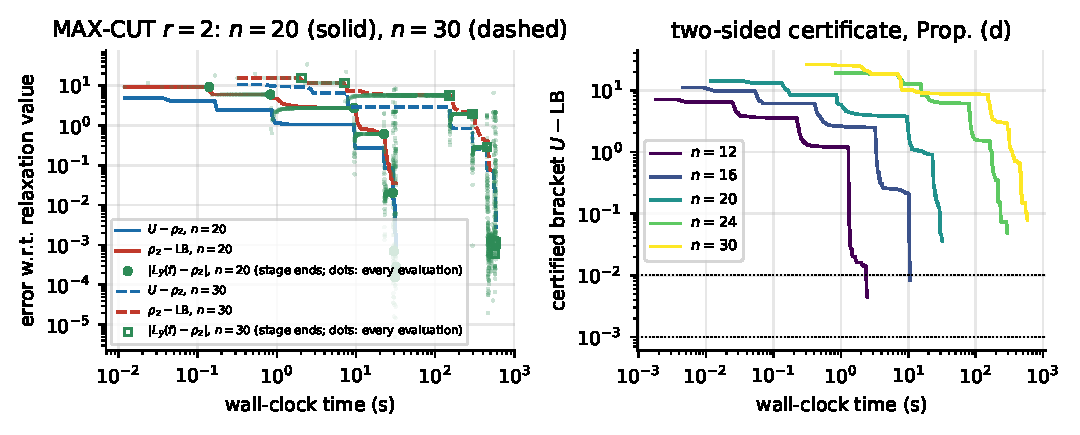
\includegraphics[width=\textwidth]{figures/primal_gap.pdf}
\caption{Left: $U-\rho_2$, $\rho_2-{\rm LB}$ and $|L_{\bar y}(f)-\rho_2|$ against time for $n=20$ (solid) and $n=30$ (dashed). Right: the certified bracket $U-{\rm LB}$ of \cref{prop:primal}(d) for all sizes (default continuation).}\label{fig:primal}
\end{figure}
\begin{table}[t]\centering\scriptsize
\setlength{\tabcolsep}{3pt}
\fitbox{\begin{tabular}{r l r r r r r r r r}\toprule
$n$ & stage & iter. & $\|g\|$ & $\rho_2-{\rm LB}$ & $U-\rho_2$ & $U-{\rm LB}$ & $t_{10^{-2}}$ & $t_{10^{-3}}$ & total (s) \\\midrule
12 & standard ($\eta\downarrow10^{-5}$) & 1149 & $2.7\cdot10^{-2}$ & $4.4\cdot10^{-3}$ & $1.0\cdot10^{-4}$ & $4.5\cdot10^{-3}$ & & & \\
 & tight $\eta=10^{-3}$ & 51 & $5.0\cdot10^{-6}$ & $4.3\cdot10^{-6}$ & $1.0\cdot10^{-4}$ & $1.1\cdot10^{-4}$ & & & \\
 & tight $\eta=3\cdot10^{-4}$ & 33 & $6.0\cdot10^{-6}$ & $4.3\cdot10^{-6}$ & $1.0\cdot10^{-4}$ & $1.1\cdot10^{-4}$ & & & \\
 & tight $\eta=10^{-4}$ & 50 & $5.4\cdot10^{-6}$ & $3.2\cdot10^{-6}$ & $1.0\cdot10^{-4}$ & $1.1\cdot10^{-4}$ & 3.15 & 3.27 & 4 \\
\addlinespace
16 & standard ($\eta\downarrow10^{-5}$) & 1116 & $1.5\cdot10^{-2}$ & $8.0\cdot10^{-3}$ & $3.1\cdot10^{-4}$ & $8.3\cdot10^{-3}$ & & & \\
 & tight $\eta=10^{-3}$ & 3000 & $4.1\cdot10^{-5}$ & $2.1\cdot10^{-5}$ & $3.1\cdot10^{-4}$ & $3.3\cdot10^{-4}$ & & & \\
 & tight $\eta=3\cdot10^{-4}$ & 28 & $1.6\cdot10^{-5}$ & $1.7\cdot10^{-5}$ & $3.1\cdot10^{-4}$ & $3.2\cdot10^{-4}$ & & & \\
 & tight $\eta=10^{-4}$ & 38 & $2.5\cdot10^{-5}$ & $1.6\cdot10^{-5}$ & $3.1\cdot10^{-4}$ & $3.2\cdot10^{-4}$ & 8.46 & 8.67 & 45 \\
\addlinespace
20 & standard ($\eta\downarrow10^{-5}$) & 1506 & $8.8\cdot10^{-2}$ & $3.5\cdot10^{-2}$ & $9.6\cdot10^{-4}$ & $3.6\cdot10^{-2}$ & & & \\
 & tight $\eta=10^{-3}$ & 3000 & $2.1\cdot10^{-3}$ & $2.2\cdot10^{-2}$ & $9.6\cdot10^{-4}$ & $2.3\cdot10^{-2}$ & & & \\
 & tight $\eta=3\cdot10^{-4}$ & 3000 & $6.3\cdot10^{-5}$ & $4.1\cdot10^{-5}$ & $9.6\cdot10^{-4}$ & $10.0\cdot10^{-4}$ & & & \\
 & tight $\eta=10^{-4}$ & 102 & $1.4\cdot10^{-4}$ & $4.1\cdot10^{-5}$ & $9.6\cdot10^{-4}$ & $10.0\cdot10^{-4}$ & 140 & 211 & 223 \\
\addlinespace
24 & standard ($\eta\downarrow10^{-5}$) & 1915 & $2.0\cdot10^{-1}$ & $4.6\cdot10^{-2}$ & $2.7\cdot10^{-3}$ & $4.9\cdot10^{-2}$ & & & \\
 & tight $\eta=10^{-3}$ & 3000 & $3.8\cdot10^{-3}$ & $3.7\cdot10^{-2}$ & $2.7\cdot10^{-3}$ & $4.0\cdot10^{-2}$ & & & \\
 & tight $\eta=3\cdot10^{-4}$ & 2150 & $2.3\cdot10^{-3}$ & $8.8\cdot10^{-4}$ & $2.7\cdot10^{-3}$ & $3.6\cdot10^{-3}$ & 771 & -- & 900 \\
\addlinespace
\bottomrule\end{tabular}
}
\caption{Tightening the stationarity: after the default continuation, L-BFGS is run to the double-precision floor on $U_\eta$ at fixed $\eta=10^{-3},3\cdot10^{-4},10^{-4}$ (at most $3000$ iterations each, $900$\,s in total). $t_{10^{-k}}$: first time at which $U-{\rm LB}<10^{-k}$, counted from the start of the run.}\label{tab:e8b}
\end{table}
The bracket ${\rm LB}\le\rho_2\le U$ held at every one of the $1187$--$2122$ evaluations per instance, $\bar y_0=1$ to $10^{-12}$, and the bound $(\sum_k\|M_k(\bar y)-X_k\|_F^2)^{1/2}\le\|g_\Theta\|$ of part (c) held at every evaluation. Two observations. First, \emph{the primal side converges faster than the certified side}: $|L_{\bar y}(f)-\rho_2|<10^{-3}$ is reached before $U-\rho_2<10^{-3}$ on every instance, and at $n=24,30$ the recovered value is within $10^{-4}$ of $\rho_2$ at $220$\,s and $464$\,s while $U-\rho_2$ is still above $10^{-2}$ (it never reaches $10^{-3}$ within the schedule). The same holds for the non-Boolean problems, where $|L_{\bar y}(f)-\rho_2^{\rm tr}|$ is $1.6\times10^{-6}$--$1.5\times10^{-4}$ at the best stage, although there $\bar y$ is infeasible by $O(\|g\|)$ and $L_{\bar y}(f)$ can overshoot $\rho^{\rm tr}_2$ (by up to $10^{-2}$ at the last stages, where $\|g\|\approx10^{-2}$). Second, the \emph{lower bound} of part (d) is the weak side of the default run: $\rho_2-{\rm LB}$ is $4\times10^{-3}$ ($n=12$) to $8\times10^{-2}$ ($n=30$), so that $U-{\rm LB}<10^{-2}$ is reached only for $n\le16$. The reason is visible in the proof: LB loses $\approx\delta\,(L_{\bar y}(f)-f_\varnothing)=\delta\,|E|/2$ with $\delta\le\|g_\Theta\|$, and the value-based stopping rule of L-BFGS leaves $\|g\|\approx10^{-2}$--$10^{-1}$ at the small-$\eta$ stages. \Cref{tab:e8b} confirms the diagnosis: running L-BFGS to the double-precision floor ($\|g\|\approx10^{-5}$) at $\eta=3\cdot10^{-4}$ and $10^{-4}$ brings $\rho_2-{\rm LB}$ down to $3$--$4\times10^{-6}$, $1.6$--$1.7\times10^{-5}$ and $4\times10^{-5}$ for $n=12,16,20$, after which the bracket $U-{\rm LB}$ equals $U-\rho_2$ within $10\%$ and the certificate is limited by the dual side only ($U-{\rm LB}<10^{-3}$ at $3.3$\,s, $8.7$\,s and $211$\,s). For $n=24$ the $900$\,s budget ran out in the $\eta=3\cdot10^{-4}$ stage ($\|g\|=2.3\times10^{-3}$, $U-{\rm LB}=3.6\times10^{-3}$). The two-sided certificate is thus practical for Boolean problems up to the sizes where the dual itself converges; its cost is one extra eigendecomposition (of $M(\bar y)$) per evaluation.

\subsection{Trace cuts, diagonal cuts and the box (E9)}\label{sec:e9}
\Cref{tab:e9a} compares the three relaxations of \cref{prop:diag}---$\rho_r$ (no cuts), $\rho_r^{\rm tr}$ (trace cuts) and $\rho_r^{\rm d}$ (diagonal cuts), all computed by an interior-point solver (Clarabel through CVXPY)---with the two first-order values: the smoothing solver (uniform shift, i.e.\ the $\rho^{\rm tr}$ side) and the dual augmented Lagrangian with the diagonal shift of \cref{prop:diag}(d) (\texttt{solve\_alm(shift="diag")}, the $\rho^{\rm d}$ side). Script \texttt{e9\_cuts.py}.
\begin{table}[t]\centering\scriptsize
\setlength{\tabcolsep}{3pt}
\fitbox{\begin{tabular}{l c c r r r r r}\toprule
Problem & $r$ & \#blocks & $\rho_r$ & $\rho_r^{\rm tr}$ & $\rho_r^{\rm d}$ & smoothing $U$ & ALM-diag $U^{\rm d}$ \\\midrule
box-free $x_1+x_2$, $x_1x_2=0$ & 1 & 1 & $+\infty$ & 1.41421 & 1.41421 & 1.41421 & 1.41421 \\
box-free $x_1+x_2$, $x_1x_2=0$ & 2 & 1 & $+\infty$ & 1.33839 & 1.18921 & 1.33839 & 1.18921 \\
box-free $x_1+x_2$, $x_1x_2=0$ & 3 & 1 & $+\infty$ & 1.28872 & 1.12246 & 1.28873 & 1.12246 \\
box QP $n=4$ (+box) & 1 & 5 & 6.33737 & 6.33737 & 6.33737 & 6.33737 & 6.33737 \\
box QP $n=4$ (no box) & 1 & 1 & $+\infty$ & 8.10130 & 6.33737 & 8.10130 & 6.33737 \\
box QP $n=4$ (+box) & 2 & 5 & 6.33737 & 6.33737 & 6.33737 & 6.33738 & 6.33737 \\
box QP $n=4$ (no box) & 2 & 1 & $+\infty$ & 7.62629 & 6.33737 & 7.62632 & 6.33737 \\
box QP $n=5$ (+box) & 1 & 6 & 8.61100 & 8.61100 & 8.61100 & 8.61102 & 8.61100 \\
box QP $n=5$ (no box) & 1 & 1 & $+\infty$ & 11.44181 & 8.61100 & 11.44183 & 8.61100 \\
box QP $n=5$ (+box) & 2 & 6 & 8.61100 & 8.61100 & 8.61100 & 8.61110 & 8.61100 \\
box QP $n=5$ (no box) & 2 & 1 & $+\infty$ & 10.98362 & 8.61100 & 10.98363 & 8.61100 \\
box QP $n=6$ (+box) & 1 & 7 & 15.44526 & 15.44526 & 15.44526 & 15.44526 & 15.44526 \\
box QP $n=6$ (no box) & 1 & 1 & $+\infty$ & 17.81941 & 15.44526 & 17.81942 & 15.44526 \\
box QP $n=6$ (+box) & 2 & 7 & 15.44526 & 15.44526 & 15.44526 & 15.44530 & 15.44526 \\
box QP $n=6$ (no box) & 2 & 1 & $+\infty$ & 17.39949 & 15.44526 & 17.39955 & 15.44526 \\
cubic on ball ($n=3$) & 2 & 2 & 1.27615 & 1.27615 & 1.27615 & 1.27617 & 1.27615 \\
cubic on ball ($n=3$) & 3 & 2 & 1.27615 & 1.27615 & 1.27615 & 1.27618 & 1.27615 \\
sphere (eq.) & 1 & 1 & 1.41421 & 1.41421 & 1.41421 & 1.41422 & 1.41421 \\
sphere (eq.) & 2 & 1 & 1.41421 & 1.41421 & 1.41421 & 1.41421 & 1.41421 \\
chain quartic $n=6$ (sparse) (+box) & 2 & 11 & 1.65685 & 1.65685 & 1.65685 & 1.65694 & 1.65685 \\
chain quartic $n=6$ (sparse) (no box) & 2 & 5 & $+\infty$ & 1.69749 & 1.65685 & 1.69757 & 1.65685 \\
MAX-CUT Petersen & 2 & 1 & 12.00000 & 12.00000 & 12.00000 & 12.00012 & 12.00000 \\
\bottomrule\end{tabular}
}
\caption{The three relaxations of \cref{prop:diag} (interior point) and the first-order values on the two sides. ``+box'' / ``no box'': with / without the explicit constraints $1-x_i^2\ge0$. $+\infty$: the solver reports unboundedness.}\label{tab:e9a}
\end{table}
\begin{table}[t]\centering\scriptsize
\setlength{\tabcolsep}{3pt}
\fitbox{% Part B: box QP (seed 1), r=2 -- 'with box constraints + uniform shift' (n+1 blocks) vs 'no box constraints + diagonal shift' (1 block)
\begin{tabular}{c r r r r r r r r r r}\toprule
 & \multicolumn{4}{c}{with box, uniform shift} & \multicolumn{4}{c}{no box, diagonal shift} & \multicolumn{2}{c}{bound} \\
\cmidrule(lr){2-5}\cmidrule(lr){6-9}\cmidrule(lr){10-11}
$n$ & blocks & mult. & smoothing $U$ (s) & ALM $U$ (s) & blocks & mult. & shifts & ALM $U^{\rm d}$ (s) & IPM $\rho_2^{\rm tr}$ & IPM $\rho_2^{\rm d}$ \\\midrule
4 & 5 & 181 & 6.33738 (0.2) & 6.33737 (0.4) & 1 & 121 & 15 & 6.33737 (0.2) & 6.33737 & 6.33737 \\
5 & 6 & 337 & 8.61110 (0.2) & 8.61101 (1.2) & 1 & 232 & 21 & 8.61100 (3.1) & 8.61100 & 8.61100 \\
6 & 7 & 575 & 15.44530 (0.8) & 15.44526 (33.3) & 1 & 407 & 28 & 15.44526 (8.3) & 15.44526 & 15.44526 \\
7 & 8 & 919 & 14.75861 (13.5) & 14.75852 (118.7) & 1 & 667 & 36 & 14.75852 (82.5) & 14.75851 & 14.75851 \\
8 & 9 & 1396 & 23.15104 (3.2) & 23.15096 (32.0) & 1 & 1036 & 45 & 23.15096 (59.3) & 23.15096 & 23.15096 \\
9 & 10 & 2036 & 33.89219 (5.1) & 33.89218 (53.2) & 1 & 1541 & 55 & 33.89218 (41.4) & 33.89218 & 33.89218 \\
10 & 11 & 2872 & 44.91238 (18.0) & 44.91235 (55.3) & 1 & 2212 & 66 & 44.91235 (66.4) & 44.91235 & 44.91235 \\
\bottomrule\end{tabular}
}
\caption{Box QP ($\max x^\top Qx$, $r=2$): the usual formulation with $n$ box constraints and the uniform shift against the formulation \emph{without} box constraints and the diagonal shift (one block, $\binom{n+2}{2}$ shift variables). Times in seconds on a shared machine (indicative only).}\label{tab:e9b}
\end{table}
Three facts emerge. (i)~Whenever the box is encoded in the constraints, or the problem is Boolean, the three relaxations coincide to solver accuracy ($\le2\times10^{-8}$) on every instance: the cuts are inactive, as observed in \cref{tab:e1}. (ii)~Without the box constraints the plain relaxation is unbounded in every case (by construction: Dirac masses at $(t,0)$ are feasible for all $t$; the interior-point \emph{status} is not always reliable, however, as a rerun of our unit test at $r=3$ on \cref{ex:boxfree} returned a spurious finite value $0.009$, below the objective of a feasible point, instead of reporting unboundedness), the trace cuts give a finite but loose value ($8.10$ against $6.34$ for the box QP with $n=4$, $r=1$), and the diagonal cuts reproduce \emph{exactly} the value of the formulation with the $n$ box constraints, at both orders and also for the correlatively sparse chain problem ($1.65685$). For \cref{ex:boxfree} the diagonal cuts are strictly tighter than the trace cuts from order $2$ on ($2^{1/4}$ and $2^{1/6}$ against $1.338$ and $1.289$). (iii)~The first-order solvers reach their respective interior-point values: the smoothing solver is within $1.2\times10^{-4}$ (median $1.5\times10^{-5}$) of $\rho^{\rm tr}$ and the diagonal-shift ALM within $6.8\times10^{-7}$ (median $7\times10^{-9}$) of $\rho^{\rm d}$, converging on every instance in $2$--$38$ outer iterations.
\Cref{tab:e9b} quantifies the structural saving for box QPs at $r=2$: dropping the $n$ localizing blocks in favour of the diagonal shift leaves one block instead of $n+1$ and $23$--$33\%$ fewer multipliers, with the same bound to $\le1.7\times10^{-6}$ for $n=4$--$10$. In time, the smoothing solver on the standard formulation remains the fastest first-order method ($0.2$--$18$\,s, accuracy $10^{-5}$--$10^{-4}$), the two ALM variants reach $10^{-6}$--$10^{-7}$ in $0.2$--$120$\,s with no uniform winner, and the interior-point solver ($0.2$--$40$\,s) is faster than both ALM variants at every $n$ and comparable to the smoothing solver (faster at $n=6,7$, slower at $n=5,8,9,10$; at $n=10$: $40$\,s against $18$\,s). The diagonal shift is therefore a modelling convenience and a tightening device when the box is not encoded, not a speed-up.

\section{Application: second-order relaxations for ReLU networks}\label{sec:nn}
Semidefinite certification of neural networks is usually limited to a first-order (Shor-type) relaxation: the SDP of Raghunathan et al.~\cite{raghunathan2018} for robustness verification, whose first-order solution at scale is the topic of~\cite{dathathri2020}, and LipSDP~\cite{fazlyab2019} for Lipschitz constants. Polynomial formulations with higher-order relaxations exist (\cite{latorre2020,chen2020lipschitz}, the latter with sparse second-order moment relaxations for Lipschitz constants), but they are limited by the cost of the SDP solver. We ask whether the first-order solvers of this paper can handle order $2$ on such problems.

\subsection{Polynomial encodings}
\paragraph{Robustness verification.} For a ReLU network $a_l=\max(W_la_{l-1}+b_l,0)$ and a $\ell_\infty$ ball around $x_0$ we maximize $c^\top(W_La_{L-1}+b_L)$ with $c=e_{\rm wrong}-e_{\rm true}$; a negative maximum proves robustness. We propagate interval bounds (IBP); \emph{stable} neurons are substituted away ($z\equiv0$ or $z=$ pre-activation), and every \emph{unstable} neuron becomes a variable $z$ with $z\ge0$, $z\ge{\rm pre}$, $z\,(z-{\rm pre})=0$ and the triangle inequality, all in the box given by IBP. The objective is linear, the constraints quadratic, so order $1$ is the Shor-type SDP of the literature and order $2$ is strictly stronger. Implemented in \texttt{moment\_sos.nn.relu\_verification}.

\paragraph{Lipschitz constants.} For $f(x)=W_1\max(W_0x+b_0,0)$, every Jacobian is $W_1\operatorname{diag}(s)W_0$ with $s\in\{0,1\}^w$, hence $\mathrm{Lip}_2(f)^2\le L_{\rm pat}^2:=\max_{\|u\|\le1,\ s\in\{0,1\}^w}\|W_1\operatorname{diag}(s)W_0u\|^2$, with equality when all activation patterns are realized. With spins $t=2s-1$ this is a POP of degree $4$ in $(u,t)$ with a ball constraint and Boolean variables $t_j$ (\cref{sec:formal}, mixed Boolean/continuous mode), so \emph{order $2$ is the lowest order that makes sense}. We compare with LipSDP-Neuron~\cite{fazlyab2019} (implemented from the LMI $\begin{psmallmatrix}-\rho I&W_0^\top T\\TW_0&W_1^\top W_1-2T\end{psmallmatrix}\preceq0$, $T$ diagonal $\ge0$, for slope-restricted $[0,1]$ activations) and with $L_{\rm pat}^2$ computed by enumeration of the $2^w$ patterns.

\subsection{Results}
\paragraph{Verification, small networks (\cref{tab:n1}).} Six small ReLU networks (two hidden layers, $d\in\{2,3,4\}$, widths $8$--$12$, trained on a synthetic classification task) were verified at a random point; the exact radius $\varepsilon^\star$ is found by bisection on a big-M MILP~\cite{tjeng2019} (HiGHS), the certified radii by bisection on the relaxation values (interior-point; the bisection depth is $9$ for order $2$ and $12$ for the exact value, so differences in the third digit are resolution). Order $2$ recovers the exact radius in all cases up to this resolution, whereas order $1$ falls short in two of six: $0.229$ against $0.233$ and, strikingly, $0.171$ against $0.227$ ($75\%$) for the network with $d=4$. At $\varepsilon=0.97\varepsilon^\star$ the order-$1$ value for that network is $+7.04$ (robustness \emph{not} certified) while the order-$2$ value is $-0.7212$, equal to the exact maximum. The ALM solver (\cref{sec:alm}) reproduces the interior-point values to $\le9\times10^{-6}$ in every case, in $4$--$62$\,s (order $2$); the smoothing solver is accurate to $10^{-2}$--$10^{-1}$ only (last column). The interior-point solver is faster on these sizes ($0.1$--$8$\,s).
\begin{table}[t]\centering\scriptsize
\setlength{\tabcolsep}{2.5pt}
\begin{tabular}{l r r r r r r r}\toprule
net $(d;\text{widths})$ & $n$ & unst. & \multicolumn{4}{c}{certified radius $\varepsilon$} \\\cmidrule(lr){4-7}
 & & & IBP & order 1 & order 2 & exact \\\midrule
$2;8{,}8$ & 9 & 7 & 0.414 & 0.494 & 0.494 & 0.494 \\
$2;10{,}10$ & 6 & 4 & 0.039 & 0.097 & 0.096 & 0.097 \\
$3;8{,}8$ & 6 & 3 & 0.010 & 0.079 & 0.078 & 0.079 \\
$3;10{,}10$ & 13 & 10 & 0.042 & 0.229 & 0.232 & 0.233 \\
$4;8{,}8$ & 14 & 10 & 0.026 & 0.171 & 0.227 & 0.227 \\
$2;12{,}12$ & 10 & 8 & 0.058 & 0.135 & 0.135 & 0.135 \\
\bottomrule\end{tabular}\par\medskip
\begin{tabular}{l r r r r r r}\toprule
net & \multicolumn{6}{c}{bound on $\max(\ell_{\rm wrong}-\ell_{\rm true})$ at $\varepsilon=0.97\,\varepsilon^\star$} \\\cmidrule(lr){2-7}
 & exact & order 1 (IPM) & order 2 (IPM) & order 1 (ALM) & order 2 (ALM) & order 2 (smooth.) \\\midrule
$2;8{,}8$ & -4.1391 & -3.8260 & -4.1391 & -3.8260 & -4.1391 & -4.1005 \\
$2;10{,}10$ & -0.4694 & -0.4694 & -0.4694 & -0.4694 & -0.4694 & -0.4691 \\
$3;8{,}8$ & -0.0531 & -0.0531 & -0.0531 & -0.0531 & -0.0531 & -0.0522 \\
$3;10{,}10$ & -0.7868 & -0.3217 & -0.7868 & -0.3217 & -0.7868 & -0.7057 \\
$4;8{,}8$ & -0.7212 & 7.0408 & -0.7212 & 7.0408 & -0.7212 & -0.6447 \\
$2;12{,}12$ & -0.4430 & -0.4430 & -0.4430 & -0.4430 & -0.4430 & -0.4305 \\
\bottomrule\end{tabular}

\caption{Robustness verification of small networks ($n$ variables after eliminating stable neurons, ``unst.'' unstable neurons). Radii: largest $\varepsilon$ with a negative bound; ``exact'' from MILP. Right block: bound on the maximal margin violation (negative = robust). ``IPM'' = interior point on the same dual (MOSEK), ``ALM'' = our dual augmented Lagrangian, ``smooth.'' = smoothing + L-BFGS.}\label{tab:n1}
\end{table}

\paragraph{Lipschitz constants (\cref{tab:n2}).} In eight networks ($w=8$--$14$, $d=3$--$5$, random and correlated weights) LipSDP-Neuron overestimates $L_{\rm pat}^2$ by $0.8\%$--$7.0\%$ (e.g.\ $1.8236$ against $1.8044$). The order-$2$ relaxation solved by ALM matches the enumerated value $L_{\rm pat}^2$ to five digits in all eight cases ($13$--$136$\,s), including the two with $n=18,19$ for which we did not run the interior-point model; the interior-point solution agrees with it where run. Order $3$ gives the same value at a much higher cost ($185$--$906$\,s) and is not needed here. Two caveats: the target $L_{\rm pat}^2$ itself bounds the true Lipschitz constant only from above (equality iff all patterns are realizable), and LipSDP is already within $7\%$ of it, so the possible improvement on these networks is small.
\begin{table}[t]\centering\scriptsize
\setlength{\tabcolsep}{3pt}
\fitbox{\begin{tabular}{l r r r r r r r r}\toprule
network & $n$ & exact $L^2_{\rm pat}$ & LipSDP & order 2 (IPM) & order 2 (ALM) & time & order 3 (ALM) & time \\\midrule
rand $d{=}3,w{=}8$ & 11 & 1.80438 & 1.82360 & 1.80438 & 1.80438 & 17\,s & 1.80438 & 249\,s \\
rand $d{=}3,w{=}8$ & 11 & 2.49374 & 2.52125 & 2.49374 & 2.49374 & 16\,s & 2.49374 & 229\,s \\
rand $d{=}3,w{=}8$ & 11 & 2.71092 & 2.85274 & 2.71092 & 2.71092 & 13\,s & 2.71092 & 185\,s \\
corr $d{=}3,w{=}10$ & 13 & 4.17584 & 4.28999 & 4.17584 & 4.17584 & 23\,s & 4.17584 & 581\,s \\
corr $d{=}4,w{=}10$ & 14 & 1.60557 & 1.70239 & 1.60557 & 1.60557 & 52\,s & 1.60557 & 906\,s \\
corr $d{=}4,w{=}12$ & 16 & 2.13059 & 2.14801 & 2.13059 & 2.13059 & 61\,s & -- & -- \\
corr $d{=}4,w{=}14$ & 18 & 3.15013 & 3.32849 & -- & 3.15013 & 97\,s & -- & -- \\
corr $d{=}5,w{=}14$ & 19 & 1.43330 & 1.53375 & -- & 1.43330 & 136\,s & -- & -- \\
\bottomrule\end{tabular}
}
\caption{Squared $\ell_2$ Lipschitz bound of one-hidden-layer ReLU networks: pattern maximum by enumeration, LipSDP-Neuron, and order-$2$/$3$ relaxations (``IPM'': interior point on the mixed Boolean/continuous problem written with equality constraints $t_j^2=1$).}\label{tab:n2}
\end{table}

\paragraph{Larger networks (\cref{tab:n3}).} We next took two-hidden-layer networks with $40$--$48$ neurons per layer (inputs $d=5,6$) and $\varepsilon$ such that $32$--$55$ neurons are unstable, i.e.\ $n=38$--$60$ variables. The dense order-$2$ relaxation has $1.1\times10^5$--$6.4\times10^5$ moments, so an interior-point Schur complement would need $\ge47$\,GiB ($n=40$: $68.7$\,GiB), beyond our machine; with correlative sparsity (blocks of size $\le120$) the $n=40$ instance has $2\times10^4$ moments and \emph{can} be solved by the interior-point solver, which we did ($1591$\,s, $19.6$\,GiB, value $-9.618$, equal to the exact maximum $-9.618$). Our ALM solver, given $1500$\,s, reaches $-8.623$ with $1.2$\,GiB: it recovers $78\%$ of the improvement of order $2$ over order $1$ ($-5.094$) in the same time as the interior-point solver and with $1/17$ of its memory, but it has \emph{not} converged (its bound was still decreasing, $0.107\to0.095$ in normalized units over the last $400$\,s). On the $n=38$ network C it reaches $8.799$ against the order-$1$ value $9.568$ and the exact maximum $8.753$ ($94\%$ of the gap closed). The smoothing solver fails on these instances (last column: its order-$2$ bounds are worse than the order-$1$ bound). On the $n=60$ network B ($55$ unstable neurons, exact maximum $11.355$, order $1$: $33.9$) the ALM solver made no useful progress in $2\,200$\,s (a single outer iteration takes about $350$\,s with $264$ blocks; its best second-order bound, $2043$, is far above the order-$1$ value), so we have \emph{no} second-order result at this size; the table entry must be read as a failure, and the order-$1$ value remains the best certificate we hold. 
\begin{table}[t]\centering\scriptsize
\setlength{\tabcolsep}{3pt}
\begin{tabular}{l r r r }\toprule
case & A: $d{=}5$, $40{\times}2$, $\varepsilon{=}0.1$ & C: $d{=}6$, $48{\times}2$, $\varepsilon{=}0.1$ & B: $d{=}5$, $40{\times}2$, $\varepsilon{=}0.2$ \\\midrule
$n$ & 40 & 38 & 60 \\
unstable neurons & 35 & 32 & 55 \\
exact maximum & -9.618 & 8.753 & 11.355 \\
order 1 (IPM) & -5.094 & 9.568 & 33.926 \\
order 1 (ALM) & -5.094 & 9.568 & 33.925 \\
order 2 sparse (IPM) & -9.618 (1591\,s, 19.6\,GiB) & not run & not run \\
order 2 sparse (ALM) & -8.623 & 8.799 & 2043.166 \\
ALM time (memory) & 1554\,s (1.2\,GiB) & 1529\,s (0.8\,GiB) & 2224\,s (3.8\,GiB) \\
smoothing, order 2 & -2.4 & 12.6 & 117.7 \\
\bottomrule\end{tabular}

\caption{Larger verification problems; $\varepsilon$ fixed so that many neurons are unstable. ``Order 2 sparse'' uses the correlative-sparsity cliques of the network. Negative = robust. The last column is the best bound of the smoothing solver within the same budget.}\label{tab:n3}
\end{table}

\paragraph{A network trained on MNIST (\cref{sec:nn}, raw data \texttt{nn\_mnist\_d4\_w8.json}).} We trained a classifier for the digits $3$ versus $8$ (MNIST, $11\,982$ training images, PCA to $d=4$ inputs scaled to $[-1,1]$, two hidden layers of width $8$, test accuracy $0.897$) and verified $8$ correctly classified test points at $\varepsilon\in\{0.05,0.1,0.2\}$ in the $\ell_\infty$ norm of the PCA coordinates ($n=4$--$15$ variables). The number of points certified robust (negative bound) is $5/3/0$ for interval bound propagation, $7/6/5$ for the order-$1$ relaxation, and $7/6/5$ for order $2$ and for the exact MILP, at $\varepsilon=0.05/0.1/0.2$. So on this network order $1$ already certifies every point that is robust. The bounds differ, however: order $1$ exceeds the exact maximum by more than $10^{-3}$ in $13$ of the $24$ cases (up to $0.49$), whereas order $2$ is exact to $2\times10^{-6}$ in all $24$. Our smoothing solver matches the interior-point values to $2.4\times10^{-2}$ (order $2$) and $2.5\times10^{-3}$ (order $1$) at $3.5$--$130$\,s, against $0.03$--$52$\,s for MOSEK; here too the interior-point solver is faster.

\paragraph{Interpretation.} The experiments support three statements. (i)~Second-order relaxations give markedly tighter certificates than the order-$1$ SDP in the networks we tried (a $33\%$ larger certified radius in one of six small networks, with robustness certified where order $1$ fails), and they are exact (to $10^{-5}$) for the Lipschitz POP of one-hidden-layer networks. (ii)~A first-order solver can compute these relaxations without a Schur complement: to $10^{-5}$ on networks with up to $n=14$ variables, and, at $n=38$--$40$ in $25$\,min, it recovers $78\%$ and $94\%$ of the order-$2$ improvement without having converged; at $n=60$ it fails. (iii)~It is \emph{not yet} a replacement for an interior-point solver on sparse relaxations of moderate size, which solved the $n=40$ instance exactly in the same time (but with $17$ times the memory), and the solver choice and the penalty parameter matter. The networks are small and trained on synthetic data, the radii come from one point per network, and the IBP boxes are loose; none of this reaches the size of networks used in practice.

\section{Discussion and limitations}\label{sec:disc}
\paragraph{What the method is good for.} It produces, at any moment of its run, a rigorous upper bound on the POP maximum, by a procedure whose memory is $O(s^2)$ instead of $O(s^4)$. When the optimum is integral and a good feasible point is available (Boolean problems), this closes the gap with a proof: the order-$2$ relaxation proves optimality of the best cut on every instance up to $n=60$ that we tried (and on all $15$ instances of \cref{sec:e10}), at sizes where the interior-point solver cannot run on the same machine; for $n\le40$ the proof is rigorous in exact arithmetic (\cref{sec:e7}). With the augmented Lagrangian the same oracle also delivers the relaxation value itself to $10^{-8}$ with a certificate, and for Boolean problems the primal recovery brackets it from both sides without any reference solver.

\paragraph{What it is not.}
(1)~It is not faster than an interior-point solver on small problems: the crossover in our experiments is at $n\approx26$ for dense order-$2$ relaxations, and for small or well-sparsified blocks MOSEK remains faster.
(2)~The accuracy of the smoothing solver is moderate: it reaches roughly $10^{-3}$--$10^{-4}$ above the relaxation value, and it is the only solver we ran at $n\ge40$. The augmented Lagrangian reaches $10^{-8}$ on MAX-CUT up to $n=30$ (\cref{sec:e10}), but it is slower to a first useful bound, depends on $\rho_0$, and was not run at larger $n$. The primal--dual bracket of \cref{prop:primal}(d) exists only for Boolean problems without constraints and is only as tight as the stationarity reached (\cref{sec:e8}); for constrained problems we recover a moment vector and its infeasibility but no lower bound on the relaxation value. The lower bounds on $f^\star$ in \cref{tab:e3} still come from local search, not from the dual iterates.
(3)~The method is not matrix-free in the strong sense: the Gram freedom has $\Theta(s^2)$ parameters, so memory is quadratic in the block size.
(4)~Our evidence for solver performance is limited: one random instance per size for $n\ge26$ (five per size for $n\le24$, \cref{sec:e10}, with a spread of about a factor $2$ in time) and wall-clock times on a shared machine. In the comparison with other first-order solvers (\cref{sec:baselines}) the non-certified baselines were faster at every size, with baseline parameters tuned per instance; we did not run SketchyCGAL with a sketch.
(5)~Engineering limits of the present code: monomials are encoded in 64-bit integers, so Boolean mode supports $n\le63$ and non-Boolean mode $n\le26$ at $r=2$; the eigen-oracle is dense up to $s\approx2500$.
(6)~The complexity theorem concerns accelerated gradient, which was the slowest solver in practice; L-BFGS, the fastest, has no guarantee here.
(7)~On the neural-network problems the second-order relaxation was solved to full accuracy only for networks with up to about $14$ variables. At $n=38$--$40$ the ALM solver had not converged after $25$\,min (for the $n=40$ case the interior-point solver on the sparse relaxation needed the same time, with $17\times$ more memory), and at $n=60$ it failed to make useful progress. The solver depends on the penalty parameter, chosen on one instance; the networks are small, trained on synthetic data, and the interval-arithmetic boxes are loose.
(7b)~\emph{Sparse MAX-CUT on library tori.} On the Biq Mac instance \texttt{t2g10} ($10\times10$ torus, $n=100$, weights up to $10^5$) the correlative-sparsity relaxation has $73$ blocks of size $\le301$. CS-TSSOS with MOSEK gives the order-$2$ value $6.0495\times10^6$ in $42$\,s but with $11$\,GB. Our smoothing solver with the default schedule stops at $6.1972\times10^6$ ($2.4\%$ above; the same value with $545$\,s and $2500$ iterations per stage as with $109$\,s) in $0.7$\,GiB. On a $5\times5$ torus with weights of the same size the two relaxations agree ($671076.875$ for ours, $671076.9999$ for TSSOS, relative $2\times10^{-7}$) and the discrepancy is smoothing bias; extending the schedule to $\eta=10^{-7}$ (\texttt{PRECISE\_ETAS}) lowers the error there from $2.2\times10^{-3}$ to $1.5\times10^{-5}$ and on \texttt{t2g10} gives $6.0497\times10^6$, $3.8\times10^{-5}$ above TSSOS, in $264$\,s. The ALM solver is slow on this instance: with warm start it did not leave the order-$1$ plateau in $400$\,s, and with its default settings it reaches only $6.76\times10^6$ ($12\%$ above) in $980$\,s, about $70$\,s per outer iteration. The best cut found by local search is $5.8707\times10^6$, so the certified relative gap is $3.0\%$, equal to the gap of the relaxation value; no optimality proof is possible. The larger tori were not run, the complete-graph \texttt{ising} instances have no sparsity to exploit, and our speed on this instance is a factor $6$ below TSSOS's with $1/15$ of the memory.
(7c)~\emph{A semismooth Newton inner solver is not competitive in our implementation.} We implemented a Newton--CG inner solver for the ALM (\texttt{inner\_solver="newton"}, exact spectral Hessian-vector products; a unit test compares it with L-BFGS-B on a Boolean and on a constrained problem). It is more accurate than L-BFGS-B on a $14$-variable verification problem ($8\times10^{-8}$ against $5\times10^{-6}$ from the interior-point value) and about $7\times$ faster for order~$1$ on \texttt{t2g10} ($11$ against $74$\,s), but on the $n=40$ network it reaches only $293.8$ in $1500$\,s (the final dual residual is still large), against $-8.623$ for L-BFGS-B and the interior-point value $-9.618$. Our first runs on this network used a version of the Newton solver that diverged on null directions of the Hessian; they were discarded and the code corrected. We have not diagnosed why the corrected solver does not converge on this problem (we suspect the truncated CG solves and the line search at large penalty parameters), so we cannot say whether a better Newton method would help at $n\ge38$.
(8)~Whenever the box is encoded in the constraints, the trace and diagonal cuts did not bind on any test problem (\cref{sec:e9}), so the box-derived weights bring no tightening over the textbook relaxation there; their benefit is confined to problems whose constraints do not imply the box (where the plain relaxation is unbounded) and to the modelling saving of \cref{tab:e9b}. The diagonal shift requires the augmented Lagrangian; we have no eigenvalue-oracle solver for it.
(9)~The rigorous certificate of \cref{thm:rigor} assumes IEEE arithmetic without underflow or overflow, certifies the bound for the floating-point problem data as given, and was run only up to $s=821$.

\paragraph{Outlook.} A spectral bundle method~\cite{helmberg2000,mai2023spectral} should combine the robustness of our oracle with faster high-accuracy convergence; term sparsity can reduce $s$ further; the oracle (one dense eigendecomposition per block) is a natural fit for GPUs; adaptively chosen weights $\varrho$ may sharpen non-Boolean relaxations; and extending the two-sided certificate of \cref{prop:primal}(d) beyond unconstrained Boolean problems (a strictly feasible moment vector with a known eigenvalue margin is all that is needed) would complete the primal--dual picture for constrained problems.

\paragraph{Reproducibility.} The package \texttt{msos} (\texttt{core.py}: construction, oracle and primal recovery; \texttt{solvers.py}: smoothing, subgradient, accelerated gradient and augmented Lagrangian; \texttt{verify.py}: rigorous certificate; \texttt{reference.py}: independent moment model with trace or diagonal cuts, MOSEK or Clarabel), the tests (\texttt{tests/}: gradient, identity, smoothing-sandwich, verification, primal-recovery, cut and ALM checks) and the scripts producing every table and figure (\texttt{experiments/}) are in the repository; raw results are in \texttt{experiments/results/}. The experiments of \cref{sec:e7,sec:e8,sec:e9,sec:e10} were run with Clarabel as the interior-point reference (MOSEK was not available on that machine), on a shared machine with three BLAS threads per run.

\appendix
\section{Proofs of the longer results}\label{app:proofs}
\begin{proof}[Proof of \cref{thm:exact}]
\emph{Conic dual.} Let $\rho_r^{\rm tr}$ be written as a conic program in $y$. Attaching multipliers $\sigma$ to $y_0=1$, $Q_{0,k},Q_i\succeq0$-type multipliers to the PSD blocks, $t_k,t_i\ge0$ to the cuts \eqref{eq:cuts} and polynomial multipliers to the equalities, and eliminating $y$ (the Lagrangian is linear in $y$), the dual is
\[
\min\ \sigma+\sum_ks_kt_k+\sum_is_iB_it_i\quad\text{s.t. \eqref{eq:identity},}\ \ Q_{0,k}+t_kI\succeq0,\ \ Q_i+t_iI\succeq0,\ \ t_i\ge0,\ t_k\ge0
\]
(in the Boolean case the trace $\tr M_k=s_k$ is an identity, the cut is an equality, and its multiplier $t_k$ is sign-free). For fixed $(\sigma,Q,p)$ the optimal $t$ is $t_k=\pos{-\lmin(Q_{0,k})}$, $t_i=\pos{-\lmin(Q_i)}$, which gives exactly $U$. (Boolean case: $\tr M_k=s_k$ holds identically, so the cut may be imposed as an equality with a free multiplier, and $t_k=-\lmin(Q_{0,k})$.)

\emph{Zero gap.} The primal feasible set is nonempty (the moment vector of a Dirac mass at a point of $K$) and bounded: the cuts bound the diagonals of the PSD blocks, and $|y_{a+b}|\le\sqrt{y_{2a}y_{2b}}$ bounds all moments. It is therefore compact and the maximum is attained. The dual is strictly feasible: \eqref{eq:identity} can be satisfied for arbitrary $(\sigma,Q_i,p_j)$ by choosing $Q_{0,k}$ as a Gram matrix of the remaining polynomial (every polynomial supported on the products of the monomials of the cliques is a Gram form), and $t_k,t_i$ can then be taken large enough for strict positive definiteness. Conic duality (e.g.~\cite[Thm.~1.4.2]{bental2001}) gives zero gap.

\emph{Remaining claims.} $\rho_r^{\rm tr}\le\rho_r$ because the cuts only add constraints, and $f^\star\le\rho_r^{\rm tr}$ because the cuts hold for Dirac measures. In the Boolean case the moment cut is an identity ($\tr M_k(y)=s_ky_0=s_k$). The localizing cut is \emph{not} an identity but is implied by the relaxation: every monomial $x^\alpha$ of $g_i$ has degree $\le 2r$ and is therefore an off-diagonal entry $y_\alpha$ of a moment block with unit diagonal, so $|y_\alpha|\le1$ and $\tr M_i^{\rm loc}(y)=s_iL_y(g_i)\le s_i\big(c_0+\sum_{\alpha\ne0}|c_\alpha|\big)\le s_iB_i$ (if $c_0<0$ the middle term is $<B_i$). Hence in the Boolean case both cuts are redundant and the two problems coincide. If an optimal solution of $\rho_r$ satisfies the cuts it is feasible for $\rho_r^{\rm tr}$. Convergence follows from Lasserre's theorem applied to the sandwiched sequence.
\end{proof}
\begin{proof}[Proof of \cref{prop:diag}]
(a) Validity: for $x$ in the box, $v^\top Qv\ge-\sum_ad_av_a^2\ge-\mathbf 1^\top d$ when $d\ge0$, with equality in the second step in the Boolean case ($v_a^2=1$), where $d$ may have any sign; the localizing terms are treated as in \cref{thm:certificate}. The block term of $U_\varrho$ is $\min\{t\,\mathbf 1^\top\varrho:\ Q+t\diag(\varrho)\succeq0,\ t\ge0\}=\min\{\mathbf 1^\top d:\ Q+\diag(d)\succeq0,\ d\in\R_+\varrho\}\ge\delta^+(Q)$. Conversely, if $d^\star$ attains $\delta^+(Q)$, the weights $\varrho=d^\star+\epsilon\mathbf1$ with $t=1$ are feasible with value $\mathbf 1^\top d^\star+\epsilon s$, so the infimum over $\varrho$ equals $\delta^+(Q)$. (For a Boolean block $t$ may be negative, but $\varrho>0$ forces all entries of $d=t\varrho$ to have the same sign, which cannot represent the mixed-sign minimizer of $\delta^0$; hence only the inequality $\delta^0(Q)\le\inf_\varrho$ is claimed there.) (b) The conic dual of the moment relaxation with diagonal cuts is obtained as in the proof of \cref{thm:exact}, with one multiplier $d_{k,a}\ge0$ per cut (free in the Boolean case, where $M_k(y)_{aa}=y_0=1$ holds identically); eliminating $y$ gives $\min U^{\rm d}$; the primal feasible set is nonempty and compact (the diagonal cuts bound every diagonal entry) and the dual is strictly feasible, so there is no gap. The diagonal cuts imply the trace cuts by summation, whence $\rho_r^{\rm d}\le\rho_r^{\rm tr}$; they hold for Dirac measures on $K$, whence $f^\star\le\rho_r^{\rm d}$. (c) In the Boolean case $M_k(y)_{aa}=y_0$ and $M_i^{\rm loc}(y)_{aa}=L_y(g_i)$ for every $a$, so the diagonal cuts coincide with the trace cuts, which are redundant by the proof of \cref{thm:exact}. (d) $(Q,d)\mapsto\mathbf 1^\top d+\iota_{\{Q+\diag d\succeq0\}}$ is jointly convex and $\delta$ is its partial minimum, so $\delta$ and $U^{\rm d}$ are convex.
\end{proof}
\begin{proof}[Proof of \cref{prop:primal}]
(a) is the Gibbs variational principle $\eta\log\tr e^{-Q/\eta}=\max\{-\iprod{Q}{P}+\eta H(P):P\succeq0,\tr P=1\}$, applied to the pencil $\diag(-Q,0)$ for the plus-version; the maximizer is the Gibbs state, which is $P_b(\theta)$. Linearity: $Q_b(\theta)=Q_b(0)+\mathcal Q_b'\theta$, and at $\theta=0$ the localizing blocks vanish while $Q_{0,k}(0)=Q^{\rm sp}(-f)$, so $\sigma-\sum_b\iprod{Q_b(\theta)}{X_b}=\iprod{\theta}{g(P)}-\sum_k\iprod{Q^{\rm sp}(-f)}{X_k}$ and $\sum_k\iprod{Q^{\rm sp}(f)}{X_k}=\sum_\gamma\frac{f_\gamma}{W_\gamma}\sum_{\operatorname{slots}(\gamma)}\omega_{ab}X_k[a,b]=L_{\bar y}(f)$ by \eqref{eq:ybar}.
(b) The partial derivatives follow from \cref{lem:gram} and $\partial_Q\,w_b\phi_{\eta,b}=-X_b$: $\partial Q_{0,k}/\partial\sigma=Q^{\rm sp}(1)$ is $1/W_0$ on the slots of the constant monomial, giving $g_\sigma=1-\bar y_0$; the moment blocks depend on $u$ and $p$ through $Q^{\rm sp}(-R_{\rm loc}u-R_{\rm eq}p)$, which produces the terms $+\omega_{ab}L_{\bar y}(g_ix^ax^b)$ and $+L_{\bar y}(h_jx^\mu)$, while the localizing block contributes $-\omega_{ab}X_i[a,b]$; the derivative with respect to a slot entry of $\Theta$ is the unit matrix of that slot, and the projection onto the zero-sum space $\{\Theta:\sum_{\operatorname{slots}(\gamma)}\omega_{ab}\Theta_{ab}=0\ \forall\gamma\}$ annihilates a vector iff it is constant on each $\operatorname{slots}(\gamma)$, i.e.\ iff $X_k[a,b]$ depends only on the product $\gamma=a\cdot b$, which is the moment structure (with common values across overlapping cliques); the $u$- and $p$-derivatives are read off from the sparse maps $R_{\rm loc},R_{\rm eq}$ in the same way. If $g=0$, $\bar y$ has $\bar y_0=1$, PSD moment and localizing blocks $X_b\succeq0$, satisfies the equalities and the trace cuts, so it is feasible for $\rho_r^{\rm tr}$ and $L_{\bar y}(f)\le\rho_r^{\rm tr}$; the identity for $L_{\bar y}(f)$ is (a) with $g=0$, and $0\le H_b\le\log(s_b+\epsilon_b)$.
(c) The inequality is (a) with the maximizer $P(\theta)$ held fixed at $\bar\theta$. Then $U(\bar\theta)\ge U_\eta(\bar\theta)-\eta\sum w_b\log(s_b+\epsilon_b)\ge U_\eta(\theta)-R\|g\|-\eta\sum w_b\log(s_b+\epsilon_b)$ and $U_\eta(\theta)\ge U(\theta)$. For the last claim, on the slots of one $\gamma$ with weights $\omega_j\in\{1,2\}$ and values $X_j$, the component of $g_\Theta$ is $-\omega_j(X_j-\tilde y_\gamma)$ (the derivative of $-w_b\iprod{Q_b}{P_b}$ projected onto the zero-sum space) with $\tilde y_\gamma$ the $\omega^2$-weighted average, and $\sum_j\omega_j(X_j-\bar y_\gamma)^2\le\sum_j\omega_j(X_j-\tilde y_\gamma)^2\le\sum_j\omega_j^2(X_j-\tilde y_\gamma)^2$ because $\bar y_\gamma$ minimizes the $\omega$-weighted sum of squares and $\omega_j\le\omega_j^2$; summing over $\gamma$ (and hence over all cliques) gives $\sum_k\|M_k(\bar y)-X_k\|_F^2\le\|g_\Theta\|^2$.
(d) $\bar y_0=\tr X/s=\tr P=1$. $\delta\le\|M(\bar y)-X\|_2\le\|g_\Theta\|$ since $X\succeq0$. The uniform measure on $\{\pm1\}^n$ has moment vector $e_\varnothing$ and moment matrix $I$ (distinct squarefree monomials are orthonormal), and $\{\pm1\}^n=K$. Thus $\tilde y=(1-\tau)\bar y+\tau e_\varnothing$ has $\tilde y_0=1$ and $M(\tilde y)=(1-\tau)M(\bar y)+\tau I\succeq\big(\tau-(1-\tau)\delta\big)I=0$, so $\tilde y$ is feasible for $\rho_r$ and $L_{\tilde y}(f)=(1-\tau)L_{\bar y}(f)+\tau f_\varnothing\le\rho_r$.
\end{proof}

\section{Additional computational results}\label{app:extra}
\subsection{Higher order (E4)}
\Cref{tab:e4} reports $r=1,2,3$ for $n=20,24$. Order $3$ gives a $1351\times1351$ ($n=20$) and $2325\times2325$ ($n=24$) block with $0.9$ and $2.7$ million multipliers, solved in $2.3$ and $3.8$\,GiB. For $n=24$ the interior-point model would have $190{,}051$ constraints and a Schur complement of $\gtrsim134$\,GiB; we did not try it. On these random $3$-regular graphs the order-$2$ relaxation is already tight, so $r=3$ does not improve the bound; the experiment only shows that certified bounds at this order are reachable on a laptop-class machine, with a larger gap to the exact value ($6\times10^{-3}$ and $2.3\times10^{-2}$ above the integer optimum) because the iteration budget is limited. We also checked with MOSEK on $G(16,\frac12)$ ($r=1$: $40.31$; $r=2,3$: $40$) and on $\pm1$-weighted complete graphs (spin glasses, $K_{14}$: $16.12\to14$; $K_{16}$: $30.58\to27$) that $r=2$ is already exact there (script \texttt{e4b\_r2\_tight.py}); we therefore make no claim that $r=3$ is needed in practice for MAX-CUT, only for structured graphs such as complete graphs.
\begin{table}[t]\centering\small
\begin{tabular}{r c r r r r r r}\toprule
$n$ & $r$ & $s$ & \#mult. & $U$ (ours) & true opt. & time & mem. \\\midrule
20 & 1 & 21 & 232 & 26.64409 & 26 & 0\,s & 0.14 \\
20 & 2 & 211 & 22{,}367 & 26.00096 & 26 & 9\,s & 0.21 \\
20 & 3 & 1351 & 913{,}277 & 26.00612 & 26 & 528\,s & 2.25 \\
24 & 2 & 301 & 45{,}452 & 32.00267 & 32 & 24\,s & 0.49 \\
24 & 3 & 2325 & 2{,}703{,}976 & 32.02266 & 32 & 2015\,s & 3.79 \\
\bottomrule\end{tabular}

\caption{Higher relaxation orders on random $3$-regular MAX-CUT; ``mem.'' in GiB. The optimum is computed by exhaustive enumeration.}\label{tab:e4}
\end{table}

\subsection{Sparsity and non-convex box QPs (E5)}
\Cref{tab:e5} shows a chain problem $\max\sum_i(a_ix_ix_{i+1}+b_ix_i^2x_{i+1}^2-0.3x_i^4)$ on the box with cliques $\{i,i+1\}$, solved with the sparse (blocks of size $6$) and the dense relaxation, and dense box QPs $\max x^\top Qx$, $x\in[-1,1]^n$. On the chain problem the sparse and dense relaxations have the same optimal value (to $5\times10^{-4}$, the solver tolerance), but the first-order method is $38\times$ faster on the sparse relaxation at $n=24$ ($1.8$\,s versus $68.5$\,s). For these small blocks \emph{MOSEK is faster than the first-order method in every row} that we ran (e.g.\ $0.4$\,s versus $1.8$\,s on the sparse chain at $n=24$), and the first-order bounds exceed the MOSEK values by up to $5.5\times10^{-4}$.
\begin{table}[t]\centering\scriptsize
\setlength{\tabcolsep}{3pt}
\fitbox{\begin{tabular}{l l r r r r r r r}\toprule
Problem & relaxation & max block & \#blocks & \#mult. & $U$ (ours) & time & MOSEK value & time \\\midrule
chain8 & sparse & 6 & 15 & 196 & 2.01419 & 0.5\,s & 2.01404 & 0.1\,s \\
chain8 & dense & 45 & 9 & 1{,}396 & 2.01427 & 1.2\,s & 2.01404 & 0.6\,s \\
chain12 & sparse & 6 & 23 & 304 & 2.37173 & 1.1\,s & 2.37146 & 0.2\,s \\
chain12 & dense & 91 & 13 & 5{,}279 & 2.37188 & 4.2\,s & 2.37146 & 2.9\,s \\
chain16 & sparse & 6 & 31 & 412 & 5.15506 & 1.3\,s & 5.15472 & 0.2\,s \\
chain16 & dense & 153 & 17 & 14{,}230 & 5.15527 & 13.3\,s & 5.15472 & 12.6\,s \\
chain20 & sparse & 6 & 39 & 520 & 7.97433 & 1.7\,s & 7.97393 & 0.3\,s \\
chain20 & dense & 231 & 21 & 31{,}417 & 7.97471 & 31.7\,s & -- & -- \\
chain24 & sparse & 6 & 47 & 628 & 8.44369 & 1.8\,s & 8.44318 & 0.4\,s \\
chain24 & dense & 325 & 25 & 60{,}776 & 8.44432 & 68.5\,s & -- & -- \\
boxqp6 & dense & 28 & 7 & 575 & 15.44530 & 0.3\,s & 15.44526 & 0.2\,s \\
boxqp8 & dense & 45 & 9 & 1{,}396 & 23.15104 & 0.7\,s & 23.15096 & 0.6\,s \\
boxqp10 & dense & 66 & 11 & 2{,}872 & 44.91237 & 1.7\,s & 44.91235 & 1.3\,s \\
boxqp12 & dense & 91 & 13 & 5{,}279 & 41.68393 & 2.8\,s & 41.68391 & 2.7\,s \\
\bottomrule\end{tabular}
}
\caption{Correlative sparsity (chain, $r=2$) and dense non-convex box QPs.}\label{tab:e5}
\end{table}


\subsection{Multi-seed structured benchmark (E5b)}\label{sec:e5b}
\Cref{tab:struct} repeats the structured problems of E5 with five seeds per size ($45$ runs; script \texttt{experiments/bench/run\_struct.py}, order $2$): dense non-convex box QPs, and the correlatively sparse chain problem solved with the sparse and with the dense relaxation. For each run the interior-point value (MOSEK, primal moment model) is the reference; we report the certified gap $U-\rho$ of the smoothing solver (default schedule) and of the dual augmented Lagrangian ($\rho_0=1000$), as median (maximum) over the seeds.
\begin{table}[t]\centering\scriptsize
\setlength{\tabcolsep}{3pt}
\fitbox{\begin{tabular}{l r r r r r r r r r}\toprule
problem & $n$ & seeds & blocks / max & IPM (s) & smoothing gap & smoothing (s) & ALM gap & ALM (s) \\\midrule
box QP & 8 & 5 & 9 / 45 & 0.69 & 7.7e-05 (4e-04) & 0.8 & 5.5e-09 (2e-07) & 0.3 \\
box QP & 10 & 5 & 11 / 66 & 1.44 & 3.4e-05 (5e-04) & 1.7 & 4.9e-08 (1e-06) & 1.0 \\
box QP & 12 & 5 & 13 / 91 & 2.77 & 3.0e-05 (2e-03) & 2.7 & 7.3e-08 (4e-07) & 2.2 \\
chain, sparse & 12 & 5 & 23 / 6 & 0.17 & 2.7e-04 (3e-04) & 0.8 & 1.7e-08 (4e-08) & 0.7 \\
chain, sparse & 16 & 5 & 31 / 6 & 0.26 & 3.5e-04 (4e-04) & 1.0 & 6.4e-08 (9e-08) & 1.0 \\
chain, sparse & 20 & 5 & 39 / 6 & 0.34 & 4.3e-04 (5e-04) & 1.5 & 2.1e-08 (3e-08) & 1.2 \\
chain, sparse & 24 & 5 & 47 / 6 & 0.44 & 5.2e-04 (5e-04) & 1.8 & 3.2e-08 (7e-08) & 1.5 \\
chain, dense & 12 & 5 & 13 / 91 & 2.83 & 4.6e-04 (7e-04) & 4.0 & 3.4e-07 (8e-07) & 7.4 \\
chain, dense & 16 & 5 & 17 / 153 & 12.27 & 8.1e-04 (9e-04) & 11.7 & 4.3e-07 (7e-07) & 37.9 \\
\bottomrule\end{tabular}
}
\caption{Structured POPs, order $2$, five seeds per row. ``blocks / max'': number of PSD blocks and the largest block size; IPM: median MOSEK time; gaps: median (maximum) of $U-\rho_2$ over the seeds; times: medians (the machine is shared, load average at the start of a run $\le4.2$).}\label{tab:struct}
\end{table}
All $90$ certified bounds are at least the interior-point value ($\ge-6\times10^{-10}$ up to solver accuracy). The smoothing solver ends $10^{-5}$--$2\times10^{-3}$ above it (maximum $2.1\times10^{-3}$), the augmented Lagrangian $10^{-9}$--$1.3\times10^{-6}$ above. On these small blocks the interior-point solver is faster in most runs: the smoothing solver is faster in $8$ of the $45$ runs and the augmented Lagrangian in $11$; the sparse chain relaxation (blocks of size $6$) is solved by the interior-point method in $0.2$--$0.4$\,s against $0.7$--$1.8$\,s. The only row where a first-order solver is on par is the dense chain with $n=16$ ($12.3$\,s for the interior-point solver, $11.7$\,s for smoothing, $37.9$\,s for the augmented Lagrangian). This confirms, over seeds, what the single-seed table of E5 showed: for blocks below about $150$ the first-order solvers do not beat an interior-point solver; their case rests on memory and on certification, not on speed at these sizes.

\subsection{Sensitivity of the smoothing solver (E13)}\label{sec:e13}
\Cref{tab:sens} varies the three tuning parameters of the smoothing solver on \texttt{g05}, $n=30$, order $2$ (three seeds, $60$ runs; script \texttt{experiments/bench/sensitivity.py}): the initial smoothing parameter $\eta_0$ (the schedule is $10^{-1},3\cdot10^{-2},\dots,10^{-5}$ truncated at $\eta_0$), the number of L-BFGS iterations per stage, and the L-BFGS memory. All $60$ runs certify the optimal cut.
\begin{table}[t]\centering\scriptsize
\setlength{\tabcolsep}{3pt}
\begin{tabular}{r r r c r r r}\toprule
$\eta_0$ & iters/stage & L-BFGS memory & certified & $t_{\rm cert}$ (s) & final gap & total (s)\\\midrule
0.1 & 200 & 30 & 3/3 & 12.7 & 1.2e-03 & 29 \\
0.1 & 500 & 30 & 3/3 & 22.4 & 1.2e-03 & 57 \\
0.1 & 1000 & 30 & 3/3 & 38.4 & 1.1e-03 & 106 \\
0.03 & 200 & 30 & 3/3 & 12.1 & 1.2e-03 & 29 \\
0.03 & 500 & 30 & 3/3 & 22.1 & 1.2e-03 & 57 \\
0.03 & 1000 & 30 & 3/3 & 37.7 & 1.2e-03 & 105 \\
0.01 & 200 & 30 & 3/3 & 7.6 & 1.2e-03 & 24 \\
0.01 & 500 & 30 & 3/3 & 17.0 & 1.2e-03 & 52 \\
0.01 & 1000 & 30 & 3/3 & 34.0 & 1.2e-03 & 102 \\
0.003 & 200 & 30 & 3/3 & 2.3 & 1.2e-03 & 19 \\
0.003 & 500 & 30 & 3/3 & 2.3 & 1.2e-03 & 37 \\
0.003 & 1000 & 30 & 3/3 & 2.3 & 1.2e-03 & 70 \\
0.001 & 200 & 30 & 3/3 & 1.0 & 1.2e-03 & 14 \\
0.001 & 500 & 30 & 3/3 & 1.0 & 1.2e-03 & 22 \\
0.001 & 1000 & 30 & 3/3 & 1.0 & 1.2e-03 & 38 \\
0.0003 & 200 & 30 & 3/3 & 1.7 & 1.1e-03 & 12 \\
0.0003 & 500 & 30 & 3/3 & 1.7 & 1.2e-03 & 18 \\
0.0003 & 1000 & 30 & 3/3 & 1.8 & 1.2e-03 & 33 \\
0.001 & 500 & 10 & 3/3 & 0.9 & 1.2e-03 & 17 \\
0.001 & 500 & 100 & 3/3 & 1.0 & 1.2e-03 & 37 \\
\bottomrule\end{tabular}

\caption{Sensitivity on \texttt{g05}, $n=30$ (median over three seeds). ``certified'': runs with $\lfloor U\rfloor=$ best cut; ``final gap'': $U-$ best cut after the whole schedule; the last row pair varies the L-BFGS memory at $\eta_0=10^{-3}$, $500$ iterations.}\label{tab:sens}
\end{table}
\emph{The initial $\eta_0$ is the dominant parameter for the time to certification}: with $500$ iterations per stage the median $t_{\rm cert}$ is $22.4$, $22.1$ and $17.0$\,s for $\eta_0=0.1,0.03,0.01$ and $2.3$, $1.0$ and $1.7$\,s for $\eta_0=3\cdot10^{-3},10^{-3},3\cdot10^{-4}$; for every $\eta_0\le3\cdot10^{-3}$ it lies between $0.32$ and $2.35$\,s over the $33$ runs. The number of iterations per stage does not change $t_{\rm cert}$ for these settings ($1.35$, $1.36$, $1.32$\,s for $200$, $500$, $1000$) but multiplies the total time; the final gap ($2.9\times10^{-4}$--$1.9\times10^{-3}$ over all runs) is essentially independent of the three parameters. The L-BFGS memory has little effect on $t_{\rm cert}$ ($0.91$, $0.98$, $0.98$\,s for memory $10$, $30$, $100$) and a memory of $100$ raises the total time from $22$ to $37$\,s. This is one family, one size and three seeds; we do not claim that these values transfer to other problems, in particular to non-Boolean ones (\cref{sec:e12}).

\section{Hand derivation versus automation}\label{app:hand}
Our starting point was a hand derivation of the dual matrices $\Sigma(\kappa,\sigma)$, $\Phi(\delta,\lambda,\sigma)$ and $\Gamma(\sigma,\lambda)$ by hand for $n=1,2$. In the present framework they are the blocks $\mathcal Q_b(\theta)$ of \cref{lem:gram}: the Hankel equalities become the zero-sum perturbations $\Theta$, the localizing relations become the entries $u$, the constant relation $y_0^2=1$ becomes the scalar $\sigma$, and the diagonal multipliers $\kappa,\mu$ of diagonal domination are replaced by the optimally chosen uniform shift $t$ (a uniform shift is the cheapest first-order-friendly choice and is exactly the dual of the trace cuts \eqref{eq:cuts}; it is tight whenever the optimal moment blocks have the maximal trace, e.g.\ in the Boolean case). \Cref{ex:ball} reproduces the ball example of that version with the correct optimum $1$ and without a spurious trace constant: with the bound $B=\sup(1-x^2)=1$ rather than $\sum|c_\alpha|=2$ the localizing weight is $s_1B=1$.


\section{Comparison with other first-order solvers: full table}
\begin{table}[h]\centering\scriptsize
\setlength{\tabcolsep}{2.5pt}
\fitbox{\begin{tabular}{r l r r r r r r r r}\toprule
$n$ & method & $t_{10^{-1}}$ & $t_{10^{-2}}$ & $t_{10^{-3}}$ & final value & signed err. & max viol. & total time & mem. \\\midrule
16 & ours (certified $U$) & 1.6\,s & 3.0\,s & 3.0\,s & 22.0003 & +3.1e-04 & $0$ & 3.1\,s & 0.18 \\
 & SCS $\epsilon{=}10^{-3}$ & 0.5\,s & 0.5\,s & n.r. & 21.9979 & -2.1e-03 & -- & 0.5\,s & 0.15 \\
 & SCS $\epsilon{=}10^{-5}$ & 0.6\,s & 0.6\,s & 0.6\,s & 22.0000 & -3.3e-07 & -- & 0.6\,s & 0.15 \\
 & CGAL & 0.1\,s & 0.2\,s & 0.5\,s & 22.0001 & +6.9e-05 & 8.4e-04 & 0.5\,s & 0.13 \\
 & BM $k{=}8$ & 0.1\,s & 0.1\,s & 0.2\,s & 22.0001 & +8.6e-05 & 9.9e-04 & 0.2\,s & 0.13 \\
 & BM $k{=}16$ & 0.2\,s & 0.2\,s & 0.3\,s & 21.9999 & -1.1e-04 & 7.9e-04 & 0.3\,s & 0.14 \\
 & MOSEK (IPM) & \multicolumn{3}{c}{(exact)} & 22.0000 & -- & -- & 0.8\,s & 0.31 \\
\midrule
20 & ours (certified $U$) & 6.3\,s & 8.3\,s & 8.6\,s & 26.0010 & +9.6e-04 & $0$ & 8.7\,s & 0.21 \\
 & SCS $\epsilon{=}10^{-3}$ & 1.5\,s & n.r. & n.r. & 25.9696 & -3.0e-02 & -- & 1.5\,s & 0.18 \\
 & SCS $\epsilon{=}10^{-5}$ & 2.3\,s & 2.3\,s & 2.3\,s & 26.0000 & -1.3e-07 & -- & 2.3\,s & 0.18 \\
 & CGAL & 0.6\,s & 2.8\,s & 8.5\,s & 25.9995 & -5.5e-04 & 9.3e-04 & 8.5\,s & 0.14 \\
 & BM $k{=}8$ & 0.3\,s & 0.5\,s & 1.4\,s & 26.0001 & +1.3e-04 & 9.9e-04 & 1.4\,s & 0.17 \\
 & BM $k{=}16$ & 0.4\,s & 1.0\,s & 1.6\,s & 26.0009 & +8.7e-04 & 9.5e-04 & 1.6\,s & 0.20 \\
 & MOSEK (IPM) & \multicolumn{3}{c}{(exact)} & 26.0000 & -- & -- & 4.1\,s & 1.00 \\
\midrule
26 & ours (certified $U$) & 17.2\,s & 26.0\,s & 26.2\,s & 36.0000 & +3.2e-05 & $0$ & 26.3\,s & 0.32 \\
 & SCS $\epsilon{=}10^{-3}$ & 6.0\,s & n.r. & n.r. & 35.9226 & -7.7e-02 & -- & 6.0\,s & 0.30 \\
 & SCS $\epsilon{=}10^{-5}$ & 9.5\,s & 9.5\,s & n.r. & 35.9982 & -1.8e-03 & -- & 9.5\,s & 0.28 \\
 & CGAL & 0.4\,s & 1.7\,s & 3.8\,s & 36.0000 & -1.8e-06 & 9.9e-04 & 3.8\,s & 0.17 \\
 & BM $k{=}8$ & 0.8\,s & 1.9\,s & 3.2\,s & 35.9996 & -4.4e-04 & 7.8e-04 & 3.2\,s & 0.26 \\
 & BM $k{=}16$ & 1.8\,s & 2.2\,s & 3.6\,s & 35.9991 & -9.3e-04 & 7.8e-04 & 3.6\,s & 0.34 \\
 & MOSEK (IPM) & \multicolumn{3}{c}{(exact)} & 36.0000 & -- & -- & 46.0\,s & 4.89 \\
\midrule
30 & ours (certified $U$) & 47.1\,s & 59.4\,s & n.r. & 40.0026 & +2.6e-03 & $0$ & 61.6\,s & 0.44 \\
 & SCS $\epsilon{=}10^{-3}$ & n.r. & n.r. & n.r. & 39.8497 & -1.5e-01 & -- & 18.7\,s & 0.38 \\
 & SCS $\epsilon{=}10^{-5}$ & 21.7\,s & 21.7\,s & 21.7\,s & 40.0000 & +2.3e-05 & -- & 21.7\,s & 0.38 \\
 & CGAL & 6.0\,s & 21.8\,s & 65.5\,s & 39.9991 & -9.3e-04 & 9.8e-04 & 65.5\,s & 0.22 \\
 & BM $k{=}8$ & 2.9\,s & 3.8\,s & 4.7\,s & 40.0003 & +2.7e-04 & 7.8e-04 & 4.7\,s & 0.35 \\
 & BM $k{=}16$ & 2.0\,s & 4.7\,s & 7.9\,s & 40.0008 & +8.5e-04 & 9.6e-04 & 7.9\,s & 0.26 \\
 & MOSEK (IPM) & \multicolumn{3}{c}{(exact)} & 40.0000 & -- & -- & 278\,s & 12.58 \\
\midrule
40 & ours (certified $U$) & 196\,s & 231\,s & 231\,s & 54.0065 & +0.0e+00 & $0$ & 241\,s & 1.04 \\
 & SCS $\epsilon{=}10^{-3}$ & n.r. & n.r. & n.r. & 53.5530 & -4.5e-01 & -- & 104\,s & 1.07 \\
 & SCS $\epsilon{=}10^{-5}$ & 129\,s & n.r. & n.r. & 53.9928 & -1.4e-02 & -- & 129\,s & 1.13 \\
 & CGAL & 16.7\,s & 177\,s & n.r. & 53.9994 & -7.1e-03 & 9.4e-04 & 445\,s & 0.42 \\
 & BM $k{=}8$ & 7.3\,s & 17.7\,s & n.r. & 54.0000 & -6.5e-03 & 9.8e-04 & 26.0\,s & 0.45 \\
 & BM $k{=}16$ & 7.6\,s & 20.3\,s & n.r. & 54.0002 & -6.3e-03 & 1.0e-03 & 37.2\,s & 0.50 \\
\bottomrule\end{tabular}
}
\caption{Order-$2$ MAX-CUT, random $3$-regular graphs. $t_{10^{-k}}$: time to reach $|{\rm value}-{\rm ref}|\le10^{-k}$ (and, for CGAL/BM, constraint violation $\le10^{-k}$); n.r.: not reached within the $1200$\,s budget. ``signed err.'' is the final value minus the reference, ``max viol.'' the final maximal constraint violation (zero for ours: certified bound). At $n=40$ the reference is our own final value $54.0065$ (MOSEK is killed). Baseline parameters were tuned per instance using the reference.}\label{tab:baselines}
\end{table}

\section*{Declarations}
% AUTHOR: please confirm or adjust every statement in this section before submission.
\paragraph{Use of AI tools.} The software, the experiments and the manuscript were developed with substantial assistance from an AI system (Claude, Anthropic), used for writing and debugging code, drafting proofs and text, and running and summarising the computations. All numbers in the paper are produced by scripts in the repository and the prose numbers are checked against the raw results by \texttt{check\_paper\_numbers.py}; the proofs were checked by the author and by AI-assisted review only, not by an independent human referee. The author is responsible for the content.
\paragraph{Code and data availability.} The package \texttt{moment\_sos}, the reference package \texttt{msos}, all experiment scripts, the raw results and the instructions to reproduce every table and figure (\texttt{REPRODUCE.md}) are in the repository [URL and archive DOI to be inserted]. The benchmark instances are generated from fixed seeds (\texttt{experiments/bench/instances.py}); no third-party data set was used.
\paragraph{Competing interests and funding.} [to be completed by the author]

\begin{thebibliography}{99}\small
\bibitem{lasserre2001} J.~B. Lasserre. Global optimization with polynomials and the problem of moments. \emph{SIAM J. Optim.} 11(3):796--817, 2001.
\bibitem{parrilo2003} P.~A. Parrilo. Semidefinite programming relaxations for semialgebraic problems. \emph{Math. Program.} 96(2):293--320, 2003.
\bibitem{laurent2009} M.~Laurent. Sums of squares, moment matrices and optimization over polynomials. In \emph{Emerging Applications of Algebraic Geometry}, IMA Vol.\ Math.\ Appl.\ 149, pp.\ 157--270. Springer, 2009.
\bibitem{nie2023} J.~Nie. \emph{Moment and Polynomial Optimization}. SIAM, 2023.
\bibitem{waki2006} H.~Waki, S.~Kim, M.~Kojima, M.~Muramatsu. Sums of squares and semidefinite program relaxations for polynomial optimization problems with structured sparsity. \emph{SIAM J. Optim.} 17(1):218--242, 2006.
\bibitem{lasserre2006} J.~B. Lasserre. Convergent SDP-relaxations in polynomial optimization with sparsity. \emph{SIAM J. Optim.} 17(3):822--843, 2006.
\bibitem{wang2021tssos} J.~Wang, V.~Magron, J.~B. Lasserre. TSSOS: A moment-SOS hierarchy that exploits term sparsity. \emph{SIAM J. Optim.} 31(1):30--58, 2021.
\bibitem{wang2022cstssos} J.~Wang, V.~Magron, J.~B. Lasserre, N.~H.~A. Mai. CS-TSSOS: Correlative and term sparsity for large-scale polynomial optimization. \emph{ACM Trans. Math. Softw.} 48(4), Art.~42, 2022.
\bibitem{mai2022ctp} N.~H.~A. Mai, J.~B. Lasserre, V.~Magron, J.~Wang. Exploiting constant trace property in large-scale polynomial optimization. \emph{ACM Trans. Math. Softw.} 48(4), Art.~40, 2022.
\bibitem{mai2023spectral} N.~H.~A. Mai, V.~Magron, J.~B. Lasserre. A hierarchy of spectral relaxations for polynomial optimization. \emph{Math. Program. Comput.} 15(4), 2023.
\bibitem{helmberg2000} C.~Helmberg, F.~Rendl. A spectral bundle method for semidefinite programming. \emph{SIAM J. Optim.} 10(3):673--696, 2000.
\bibitem{lewis1996} A.~S. Lewis, M.~L. Overton. Eigenvalue optimization. \emph{Acta Numerica} 5:149--190, 1996.
\bibitem{dathathri2020} S.~Dathathri, K.~Dvijotham, A.~Kurakin, A.~Raghunathan, J.~Uesato, R.~Bunel, S.~Shankar, J.~Steinhardt, I.~Goodfellow, P.~Liang, P.~Kohli. Enabling certification of verification-agnostic networks via memory-efficient semidefinite programming. \emph{NeurIPS} 33, 2020.
\bibitem{nesterov2005} Yu.~Nesterov. Smooth minimization of non-smooth functions. \emph{Math. Program.} 103(1):127--152, 2005.
\bibitem{nesterov2007} Yu.~Nesterov. Smoothing technique and its applications in semidefinite optimization. \emph{Math. Program.} 110(2):245--259, 2007.
\bibitem{beck2009} A.~Beck, M.~Teboulle. A fast iterative shrinkage-thresholding algorithm for linear inverse problems. \emph{SIAM J. Imaging Sci.} 2(1):183--202, 2009.
\bibitem{goemans1995} M.~X. Goemans, D.~P. Williamson. Improved approximation algorithms for maximum cut and satisfiability problems using semidefinite programming. \emph{J. ACM} 42(6):1115--1145, 1995.
\bibitem{laurent2003} M.~Laurent. Lower bound for the number of iterations in semidefinite hierarchies for the cut polytope. \emph{Math. Oper. Res.} 28(4):871--883, 2003.
\bibitem{odonoghue2016} B.~O'Donoghue, E.~Chu, N.~Parikh, S.~Boyd. Conic optimization via operator splitting and homogeneous self-dual embedding. \emph{J. Optim. Theory Appl.} 169(3):1042--1068, 2016.
\bibitem{zheng2020} Y.~Zheng, G.~Fantuzzi, A.~Papachristodoulou, P.~Goulart, A.~Wynn. Chordal decomposition in operator-splitting methods for sparse semidefinite programs. \emph{Math. Program.} 180:489--532, 2020.
\bibitem{yurtsever2021} A.~Yurtsever, J.~A. Tropp, O.~Fercoq, M.~Udell, V.~Cevher. Scalable semidefinite programming. \emph{SIAM J. Math. Data Sci.} 3(1):171--200, 2021.
\bibitem{burer2003} S.~Burer, R.~D.~C. Monteiro. A nonlinear programming algorithm for solving semidefinite programs via low-rank factorization. \emph{Math. Program.} 95(2):329--357, 2003.
\bibitem{hou2025} D.~Hou, T.~Tang, K.-C. Toh. A low-rank augmented Lagrangian method for polyhedral-SDP and moment-SOS relaxations of polynomial optimization. arXiv:2512.06359, 2025.
\bibitem{wang2023manisdp} J.~Wang, L.~Hu. Solving low-rank semidefinite programs via manifold optimization. \emph{J. Sci. Comput.}, 2025, doi:10.1007/s10915-025-02952-8 (arXiv:2303.01722).
\bibitem{raghunathan2018} A.~Raghunathan, J.~Steinhardt, P.~Liang. Semidefinite relaxations for certifying robustness to adversarial examples. \emph{NeurIPS} 31, 2018.
\bibitem{fazlyab2019} M.~Fazlyab, A.~Robey, H.~Hassani, M.~Morari, G.~J. Pappas. Efficient and accurate estimation of Lipschitz constants for deep neural networks. \emph{NeurIPS} 32, 2019.
\bibitem{latorre2020} F.~Latorre, P.~Rolland, V.~Cevher. Lipschitz constant estimation of neural networks via sparse polynomial optimization. \emph{ICLR}, 2020 (arXiv:2004.08688).
\bibitem{chen2020lipschitz} T.~Chen, J.-B. Lasserre, V.~Magron, E.~Pauwels. Semialgebraic optimization for Lipschitz constants of ReLU networks. \emph{NeurIPS} 33, 2020 (arXiv:2002.03657).
\bibitem{tjeng2019} V.~Tjeng, K.~Xiao, R.~Tedrake. Evaluating robustness of neural networks with mixed integer programming. \emph{ICLR}, 2019 (arXiv:1711.07356).
\bibitem{zhao2010} X.-Y. Zhao, D.~Sun, K.-C. Toh. A Newton-CG augmented Lagrangian method for semidefinite programming. \emph{SIAM J. Optim.} 20(4):1737--1765, 2010.
\bibitem{povh2006} J.~Povh, F.~Rendl, A.~Wiegele. A boundary point method to solve semidefinite programs. \emph{Computing} 78(3):277--286, 2006.
\bibitem{malick2009} J.~Malick, J.~Povh, F.~Rendl, A.~Wiegele. Regularization methods for semidefinite programming. \emph{SIAM J. Optim.} 20(1):336--356, 2009.
\bibitem{henrion2009} D.~Henrion, J.~B. Lasserre, J.~L\"ofberg. GloptiPoly 3: moments, optimization and semidefinite programming. \emph{Optim. Methods Softw.} 24(4--5):761--779, 2009.
\bibitem{papachristodoulou2013} A.~Papachristodoulou et al. SOSTOOLS version 4.00. arXiv:1310.4716.
\bibitem{waki2008sparsepop} H.~Waki, S.~Kim, M.~Kojima, M.~Muramatsu, H.~Sugimoto. Algorithm 883: SparsePOP---a sparse semidefinite programming relaxation of polynomial optimization problems. \emph{ACM Trans. Math. Softw.}, 2008, doi:10.1145/1377612.1377619.
\bibitem{magron2021tssos} V.~Magron, J.~Wang. TSSOS: a Julia library to exploit sparsity for large-scale polynomial optimization. arXiv:2103.00915.
\bibitem{wittek2015} P.~Wittek. Algorithm 950: Ncpol2sdpa---sparse semidefinite programming relaxations for polynomial optimization problems of noncommuting variables. \emph{ACM Trans. Math. Softw.} 41(3), Art.~21, 2015.
\bibitem{kang2024} Kang, Xu, Sarva, Liang, Yang. Fast and certifiable trajectory optimization. arXiv:2406.05846, 2024.
\bibitem{wiegele2007} A.~Wiegele. Biq Mac library---a collection of Max-Cut and quadratic 0-1 programming instances of medium size. Preprint, 2007 (\url{https://biqmac.aau.at/}).
\bibitem{bental2001} A.~Ben-Tal, A.~Nemirovski. \emph{Lectures on Modern Convex Optimization}. SIAM, 2001.
\bibitem{higham2002} N.~J. Higham. \emph{Accuracy and Stability of Numerical Algorithms}. 2nd ed., SIAM, 2002.
\bibitem{jansson2008} C.~Jansson, D.~Chaykin, C.~Keil. Rigorous error bounds for the optimal value in semidefinite programming. \emph{SIAM J. Numer. Anal.} 46(1):180--200, 2008.
\bibitem{peyrl2008} H.~Peyrl, P.~A. Parrilo. Computing sum of squares decompositions with rational coefficients. \emph{Theoret. Comput. Sci.} 409(2):269--281, 2008.
\end{thebibliography}
\end{document}
